% Options for packages loaded elsewhere
\PassOptionsToPackage{unicode}{hyperref}
\PassOptionsToPackage{hyphens}{url}
\PassOptionsToPackage{dvipsnames,svgnames,x11names}{xcolor}
%
\documentclass[
  letterpaper,
  DIV=11,
  numbers=noendperiod]{scrreprt}

\usepackage{amsmath,amssymb}
\usepackage{iftex}
\ifPDFTeX
  \usepackage[T1]{fontenc}
  \usepackage[utf8]{inputenc}
  \usepackage{textcomp} % provide euro and other symbols
\else % if luatex or xetex
  \usepackage{unicode-math}
  \defaultfontfeatures{Scale=MatchLowercase}
  \defaultfontfeatures[\rmfamily]{Ligatures=TeX,Scale=1}
\fi
\usepackage{lmodern}
\ifPDFTeX\else  
    % xetex/luatex font selection
\fi
% Use upquote if available, for straight quotes in verbatim environments
\IfFileExists{upquote.sty}{\usepackage{upquote}}{}
\IfFileExists{microtype.sty}{% use microtype if available
  \usepackage[]{microtype}
  \UseMicrotypeSet[protrusion]{basicmath} % disable protrusion for tt fonts
}{}
\makeatletter
\@ifundefined{KOMAClassName}{% if non-KOMA class
  \IfFileExists{parskip.sty}{%
    \usepackage{parskip}
  }{% else
    \setlength{\parindent}{0pt}
    \setlength{\parskip}{6pt plus 2pt minus 1pt}}
}{% if KOMA class
  \KOMAoptions{parskip=half}}
\makeatother
\usepackage{xcolor}
\setlength{\emergencystretch}{3em} % prevent overfull lines
\setcounter{secnumdepth}{5}
% Make \paragraph and \subparagraph free-standing
\makeatletter
\ifx\paragraph\undefined\else
  \let\oldparagraph\paragraph
  \renewcommand{\paragraph}{
    \@ifstar
      \xxxParagraphStar
      \xxxParagraphNoStar
  }
  \newcommand{\xxxParagraphStar}[1]{\oldparagraph*{#1}\mbox{}}
  \newcommand{\xxxParagraphNoStar}[1]{\oldparagraph{#1}\mbox{}}
\fi
\ifx\subparagraph\undefined\else
  \let\oldsubparagraph\subparagraph
  \renewcommand{\subparagraph}{
    \@ifstar
      \xxxSubParagraphStar
      \xxxSubParagraphNoStar
  }
  \newcommand{\xxxSubParagraphStar}[1]{\oldsubparagraph*{#1}\mbox{}}
  \newcommand{\xxxSubParagraphNoStar}[1]{\oldsubparagraph{#1}\mbox{}}
\fi
\makeatother

\usepackage{color}
\usepackage{fancyvrb}
\newcommand{\VerbBar}{|}
\newcommand{\VERB}{\Verb[commandchars=\\\{\}]}
\DefineVerbatimEnvironment{Highlighting}{Verbatim}{commandchars=\\\{\}}
% Add ',fontsize=\small' for more characters per line
\usepackage{framed}
\definecolor{shadecolor}{RGB}{241,243,245}
\newenvironment{Shaded}{\begin{snugshade}}{\end{snugshade}}
\newcommand{\AlertTok}[1]{\textcolor[rgb]{0.68,0.00,0.00}{#1}}
\newcommand{\AnnotationTok}[1]{\textcolor[rgb]{0.37,0.37,0.37}{#1}}
\newcommand{\AttributeTok}[1]{\textcolor[rgb]{0.40,0.45,0.13}{#1}}
\newcommand{\BaseNTok}[1]{\textcolor[rgb]{0.68,0.00,0.00}{#1}}
\newcommand{\BuiltInTok}[1]{\textcolor[rgb]{0.00,0.23,0.31}{#1}}
\newcommand{\CharTok}[1]{\textcolor[rgb]{0.13,0.47,0.30}{#1}}
\newcommand{\CommentTok}[1]{\textcolor[rgb]{0.37,0.37,0.37}{#1}}
\newcommand{\CommentVarTok}[1]{\textcolor[rgb]{0.37,0.37,0.37}{\textit{#1}}}
\newcommand{\ConstantTok}[1]{\textcolor[rgb]{0.56,0.35,0.01}{#1}}
\newcommand{\ControlFlowTok}[1]{\textcolor[rgb]{0.00,0.23,0.31}{\textbf{#1}}}
\newcommand{\DataTypeTok}[1]{\textcolor[rgb]{0.68,0.00,0.00}{#1}}
\newcommand{\DecValTok}[1]{\textcolor[rgb]{0.68,0.00,0.00}{#1}}
\newcommand{\DocumentationTok}[1]{\textcolor[rgb]{0.37,0.37,0.37}{\textit{#1}}}
\newcommand{\ErrorTok}[1]{\textcolor[rgb]{0.68,0.00,0.00}{#1}}
\newcommand{\ExtensionTok}[1]{\textcolor[rgb]{0.00,0.23,0.31}{#1}}
\newcommand{\FloatTok}[1]{\textcolor[rgb]{0.68,0.00,0.00}{#1}}
\newcommand{\FunctionTok}[1]{\textcolor[rgb]{0.28,0.35,0.67}{#1}}
\newcommand{\ImportTok}[1]{\textcolor[rgb]{0.00,0.46,0.62}{#1}}
\newcommand{\InformationTok}[1]{\textcolor[rgb]{0.37,0.37,0.37}{#1}}
\newcommand{\KeywordTok}[1]{\textcolor[rgb]{0.00,0.23,0.31}{\textbf{#1}}}
\newcommand{\NormalTok}[1]{\textcolor[rgb]{0.00,0.23,0.31}{#1}}
\newcommand{\OperatorTok}[1]{\textcolor[rgb]{0.37,0.37,0.37}{#1}}
\newcommand{\OtherTok}[1]{\textcolor[rgb]{0.00,0.23,0.31}{#1}}
\newcommand{\PreprocessorTok}[1]{\textcolor[rgb]{0.68,0.00,0.00}{#1}}
\newcommand{\RegionMarkerTok}[1]{\textcolor[rgb]{0.00,0.23,0.31}{#1}}
\newcommand{\SpecialCharTok}[1]{\textcolor[rgb]{0.37,0.37,0.37}{#1}}
\newcommand{\SpecialStringTok}[1]{\textcolor[rgb]{0.13,0.47,0.30}{#1}}
\newcommand{\StringTok}[1]{\textcolor[rgb]{0.13,0.47,0.30}{#1}}
\newcommand{\VariableTok}[1]{\textcolor[rgb]{0.07,0.07,0.07}{#1}}
\newcommand{\VerbatimStringTok}[1]{\textcolor[rgb]{0.13,0.47,0.30}{#1}}
\newcommand{\WarningTok}[1]{\textcolor[rgb]{0.37,0.37,0.37}{\textit{#1}}}

\providecommand{\tightlist}{%
  \setlength{\itemsep}{0pt}\setlength{\parskip}{0pt}}\usepackage{longtable,booktabs,array}
\usepackage{calc} % for calculating minipage widths
% Correct order of tables after \paragraph or \subparagraph
\usepackage{etoolbox}
\makeatletter
\patchcmd\longtable{\par}{\if@noskipsec\mbox{}\fi\par}{}{}
\makeatother
% Allow footnotes in longtable head/foot
\IfFileExists{footnotehyper.sty}{\usepackage{footnotehyper}}{\usepackage{footnote}}
\makesavenoteenv{longtable}
\usepackage{graphicx}
\makeatletter
\newsavebox\pandoc@box
\newcommand*\pandocbounded[1]{% scales image to fit in text height/width
  \sbox\pandoc@box{#1}%
  \Gscale@div\@tempa{\textheight}{\dimexpr\ht\pandoc@box+\dp\pandoc@box\relax}%
  \Gscale@div\@tempb{\linewidth}{\wd\pandoc@box}%
  \ifdim\@tempb\p@<\@tempa\p@\let\@tempa\@tempb\fi% select the smaller of both
  \ifdim\@tempa\p@<\p@\scalebox{\@tempa}{\usebox\pandoc@box}%
  \else\usebox{\pandoc@box}%
  \fi%
}
% Set default figure placement to htbp
\def\fps@figure{htbp}
\makeatother

\KOMAoption{captions}{tableheading}
\makeatletter
\@ifpackageloaded{bookmark}{}{\usepackage{bookmark}}
\makeatother
\makeatletter
\@ifpackageloaded{caption}{}{\usepackage{caption}}
\AtBeginDocument{%
\ifdefined\contentsname
  \renewcommand*\contentsname{Tabla de contenidos}
\else
  \newcommand\contentsname{Tabla de contenidos}
\fi
\ifdefined\listfigurename
  \renewcommand*\listfigurename{Listado de Figuras}
\else
  \newcommand\listfigurename{Listado de Figuras}
\fi
\ifdefined\listtablename
  \renewcommand*\listtablename{Listado de Tablas}
\else
  \newcommand\listtablename{Listado de Tablas}
\fi
\ifdefined\figurename
  \renewcommand*\figurename{Figura}
\else
  \newcommand\figurename{Figura}
\fi
\ifdefined\tablename
  \renewcommand*\tablename{Tabla}
\else
  \newcommand\tablename{Tabla}
\fi
}
\@ifpackageloaded{float}{}{\usepackage{float}}
\floatstyle{ruled}
\@ifundefined{c@chapter}{\newfloat{codelisting}{h}{lop}}{\newfloat{codelisting}{h}{lop}[chapter]}
\floatname{codelisting}{Listado}
\newcommand*\listoflistings{\listof{codelisting}{Listado de Listados}}
\makeatother
\makeatletter
\makeatother
\makeatletter
\@ifpackageloaded{caption}{}{\usepackage{caption}}
\@ifpackageloaded{subcaption}{}{\usepackage{subcaption}}
\makeatother

\ifLuaTeX
\usepackage[bidi=basic]{babel}
\else
\usepackage[bidi=default]{babel}
\fi
\babelprovide[main,import]{spanish}
% get rid of language-specific shorthands (see #6817):
\let\LanguageShortHands\languageshorthands
\def\languageshorthands#1{}
\usepackage{bookmark}

\IfFileExists{xurl.sty}{\usepackage{xurl}}{} % add URL line breaks if available
\urlstyle{same} % disable monospaced font for URLs
\hypersetup{
  pdftitle={ApLabAD},
  pdfauthor={RICUIB},
  pdflang={es},
  colorlinks=true,
  linkcolor={blue},
  filecolor={Maroon},
  citecolor={Blue},
  urlcolor={Blue},
  pdfcreator={LaTeX via pandoc}}


\title{ApLabAD}
\usepackage{etoolbox}
\makeatletter
\providecommand{\subtitle}[1]{% add subtitle to \maketitle
  \apptocmd{\@title}{\par {\large #1 \par}}{}{}
}
\makeatother
\subtitle{Apuntes de Laboratorio de Análisis de Datos}
\author{RICUIB}
\date{2025-02-01}

\begin{document}
\maketitle

\renewcommand*\contentsname{Tabla de contenidos}
{
\hypersetup{linkcolor=}
\setcounter{tocdepth}{2}
\tableofcontents
}

\bookmarksetup{startatroot}

\chapter*{Prefacio}\label{prefacio}
\addcontentsline{toc}{chapter}{Prefacio}

\markboth{Prefacio}{Prefacio}

Este libro en la web es una versión de las notas de clase de asignaturas
introductorias al análisis de datos.

\begin{description}
\item[Ha sido elaborado con \href{https://quarto.org/}{Quarto}]
RStudio, PBC. (2022). Quarto (Version 1.0). Hemos utilizado el formato
formato book.
\end{description}

\part{Parte 1: Probabilidad y variables aleatorias}

En esta sección, veremos la teoría básica de la probabilidad y de las
variables aleatorias. Resolveremos problemas prácticos para comprender
mejor los conceptos y utilizaremos R para realizar cálculos y gráficos.

También exploraremos los modelos de probabilidad discretos y continuos
más conocidos.

En ocasiones, trabajaremos con problemas de cálculo más complejos.

Además, introduciremos problemas sencillos de modelización con
probabilidades. Estos consistirán en un enunciado, real o inventado, en
el que se pedirá modelizar el problema mediante una variable aleatoria y
responder a una serie de preguntas.

\chapter{Preliminares: conjuntos y
combinatoria}\label{preliminares-conjuntos-y-combinatoria}

Para aprender cálculo de probabilidades son necesarios conocimientos de:

\begin{enumerate}
\def\labelenumi{\arabic{enumi}.}
\tightlist
\item
  Cálculo: Derivadas, integrales, límites, sumas de series\ldots{}
\item
  Geometría básica y álgebra lineal : rectas, hiperplanos,
  volúmenes\ldots{} Matrices, valores propios\ldots{}
\item
  Teoría de conjuntos y combinatoria\ldots..
\end{enumerate}

Por experiencia sabemos que la mayoría de estudiantes tienen más
conocimientos de cálculo, geometría y matrices.

Pero muchos tienen una falta de conocimientos en teoría básica de
conjuntos y combinatoria (matemática discreta).

\section{Teoría de conjuntos}\label{teoruxeda-de-conjuntos}

Definición de conjunto

La definición de conjunto es una
\href{https://es.wikipedia.org/wiki/Concepto_primitivo}{idea o noción
primitiva}. Es decir es una idea básica del pensamiento humano: un
conjunto es una colección de objetos: números, imágenes\ldots{}
cualquier cosa, jugadores de fútbol, palabras, colores \ldots.

La definición de conjunto es una
\href{https://es.wikipedia.org/wiki/Concepto_primitivo}{idea o noción
primitiva}. Es decir es una idea básica del pensamiento humano: un
conjunto es una colección de objetos: números, imágenes\ldots{}
cualquier cosa, jugadores de fútbol, palabras, colores \ldots.

La teoría de conjuntos básicas es simple y natural y es la que
necesitamos para este curso.

La teoría de conjuntos matemática es más compleja y presenta varias
paradojas como la
\href{https://es.wikipedia.org/wiki/Paradoja_de_Russell}{paradoja de
Russell}.

La idea o noción práctica de conjunto es la de una colección de objetos
de un cierto tipo.

Estas colecciones o conjuntos se pueden definir por:

\begin{itemize}
\tightlist
\item
  \textbf{Comprensión}: reuniendo los objetos que cumplen una propiedad
  \(p\)
\item
  \textbf{Extensión}: dando una lista exhaustiva de los miembros del
  conjunto
\end{itemize}

\subsection{Conjuntos básicos}\label{conjuntos-buxe1sicos}

Los conjuntos suelen tener un conjunto madre como por ejemplo

\begin{itemize}
\item
  \(\mathbb{N}=\{0,1,2,\ldots\}\)
\item
  \(\mathbb{Z}=\{\ldots,-2,-1,0,1,2,\ldots\}\)
\item
  \(\mathbb{Q}=\left\{\frac{p}{q}\quad\Big|\quad p,q\in \mathbb{Z} \mbox{ y } q \not= 0.\right\}\)
\item
  \(\mathbb{R}=\{\mbox{Todos los puntos de una recta.}\}\)
\item
  \(\mathbb{C}= \left\{a+b\cdot i\quad \big|\quad a,b\in \mathbb{R}\right\}\mbox{ los números complejos}\quad a+b\cdot i.\)
\item
  Alfabeto = \(\{a,b,c,\ldots, A,B,C,\ldots\}.\)
\item
  Palabras = \(\{paz, guerra, amor, probabilidad,\ldots\}.\)
\end{itemize}

Recordemos que \(i\) es la unidad imaginaria que cumple que
\(i=\sqrt{-1}\).

\subsection{Características y propiedades básicas de los
conjuntos}\label{caracteruxedsticas-y-propiedades-buxe1sicas-de-los-conjuntos}

Si a cada objeto \(x\) de \(\Omega\) le llamaremos \textbf{elemento del
conjunto} \(\Omega\) y diremos que \(x\) pertenece a \(\Omega\). Lo
denotaremos por \(x\in \Omega\).

Un \textbf{conjunto de un elemento}, por ejemplo \(\{1\}\) recibe el
nombre de \textbf{conjunto elemental} (o \textbf{singleton} del inglés).

Sea \(A\) otro conjunto diremos que \(A\) \textbf{es igual a} \(B\) si
todos los elementos \(A\) están en \(B\) y todos los elementos de \(B\)
están en \(A\). Por ejemplo \(A=\{1,2,3\}\) es igual a \(B=\{3,1,2\}\).

Si \(B\) es otro conjunto, tal que si \(x\in A\) entonces \(x\in B\)
diremos que \(A\) es un subconjunto de o que está contenido en \(B\). Lo
denotaremos por \(A\subseteq B.\)

El conjunto que no tiene elementos se denomina conjunto vacío y se
denota por el símbolo \(\emptyset\). Dado \(A\) un conjunto cualquiera
obviamente \(\emptyset\subseteq A.\)

Ejemplo

Tomemos como conjunto base \(\Omega=\{1,2,3\}\)

\begin{itemize}
\tightlist
\item
  \(\Omega\) es un conjunto de cardinal 3, se denota por
  \(\#(\Omega)=3\) o por \(|\Omega|=3\)
\item
  El conjunto \(\Omega\) tiene \(2^3=8\) subconjuntos.

  \begin{itemize}
  \tightlist
  \item
    el vacío \(\emptyset\) y los elementales \(\{1\},\{2\},\{3\}\)
  \item
    los subconjuntos de dos elementos: \(\{1,2\},\{1,3\},\{2,3\}\)
  \item
    el conjunto total de tres elementos \(\Omega=\{1,2,3\}.\)
  \end{itemize}
\end{itemize}

Dado un conjunto \(\Omega\) podemos construir el \textbf{conjunto de
todas sus partes} (todos sus subconjuntos) al que denotamos por
\(\mathcal{P}(\Omega)\). También se denomina de forma directa partes de
\(\Omega\).

Cardinal de las partes de un conjunto

Propiedad

Por ejemplo
\(\#\left(\mathcal{P}(\{1,2,3\})\right)=2^{\#(\{1,2,3\})}=2^3=8.\)

Efectivamente

\[\mathcal{P}(\{1,2,3\})=\{\emptyset,\{1\},\{2\},\{3\},\{1,2\},\{1,3\},\{2,3\},\{1,2,3\}\}.\]

Dado un subconjunto \(A\) de \(\Omega\) podemos construir la función
característica de \(A\) \[\chi_A:\Omega \to \{0,1\}\]

dado un \(\omega\in \Omega\)

\[
\chi_A(\omega)=
\left\{
\begin{array}{ll}
1 &  \mbox{si }\omega \in A\\
0 &  \mbox{si }\omega \not\in A
\end{array}
\right.
\]

\subsection{Operaciones entre
conjuntos}\label{operaciones-entre-conjuntos}

\textbf{Intersección}

Sea \(\Omega\) un conjunto y \(A\) y \(B\) dos subconjuntos de
\(\Omega\).

El conjunto \textbf{intersección} de \(A\) y \(B\) es el formado por
todos los elementos que perteneces a \(A\) \textbf{Y} \(B\), se denota
por \(A\cap B\).

Más formalmente

\[
A\cap B=\left\{x\in\Omega \big| x\in A \mbox{ y } x\in B\right\}.
\]

\textbf{Unión}

El conjunto \textbf{unión} de \(A\) y \(B\) es el formado por todos los
elementos que perteneces a \(A\) \textbf{O} pertenecen a \(B\), se
denota por \(A\cup B\).

Más formalmente

\[
A\cup B=\left\{x\in\Omega \big| x\in A \mbox{ o } x\in B\right\}.
\]

Diferencia.

El conjunto \textbf{diferencia} de \(A\) y \(B\) es el formado por todos
los elementos que perteneces a \(A\) \textbf{Y NO} pertenecen a \(B\),
se denota por \(A-B=A-(A\cap B)\).

Más formalmente

\[
A- B=\left\{x\in\Omega \big| x\in A \mbox{ y } x\notin B\right\}.
\]

Complementario

El \textbf{complementario} de un subconjunto \(A\) de \(\Omega\) es
\(\Omega-A\) y se denota por \(A^c\) o \(\overline{A}\).

Más formalmente

\[
A^c=\left\{x\in\Omega \big| x\not\in A\right\}.
\]

\subsection{Más propiedades}\label{muxe1s-propiedades}

Sea \(\Omega\) un conjunto y \(A\), \(B\), \(C\) tres subconjuntos de
\(\Omega\)

\begin{itemize}
\tightlist
\item
  Se dice que dos conjuntos \(A\) y \(B\) \textbf{son disjuntos} si
  \(A\cap B=\emptyset.\)
\item
  \(\Omega^c=\emptyset\).
\item
  \(\emptyset^c=\Omega\).
\item
  \(A\cup B=B \cup A\) , \(A\cap B=B\cap A\) conmutativas.
\item
  \((A\cup B) \cup C = A \cup( B \cup C)\) ,
  \((A\cap B) \cap C = A \cap( B \cap C)\) asociativas.
\item
  \(A\cup (B\cap C)=(A\cup B) \cap (A\cup C)\) ,
  \(A\cap (B\cup C)=(A\cap B) \cup (A\cap C)\) distributivas.
\item
  \(\left(A^c\right)^c=A\) doble complementario.
\item
  \(\left(A\cup B\right)^c=A^c \cap B^c\),
  \(\left(A\cap B\right)^c=A^c \cup B^c\)
  \href{https://es.wikipedia.org/wiki/Leyes_de_De_Morgan}{leyes de De
  Morgan}.
\end{itemize}

\subsection{Con R, ejemplos.}\label{con-r-ejemplos.}

Con R los conjuntos de pueden definir como vectores

\begin{Shaded}
\begin{Highlighting}[]
\NormalTok{Omega}\OtherTok{=}\FunctionTok{c}\NormalTok{(}\DecValTok{1}\NormalTok{,}\DecValTok{2}\NormalTok{,}\DecValTok{3}\NormalTok{,}\DecValTok{4}\NormalTok{,}\DecValTok{5}\NormalTok{,}\DecValTok{6}\NormalTok{,}\DecValTok{7}\NormalTok{,}\DecValTok{8}\NormalTok{,}\DecValTok{9}\NormalTok{,}\DecValTok{10}\NormalTok{)}
\NormalTok{A}\OtherTok{=}\FunctionTok{c}\NormalTok{(}\DecValTok{1}\NormalTok{,}\DecValTok{2}\NormalTok{,}\DecValTok{3}\NormalTok{,}\DecValTok{4}\NormalTok{,}\DecValTok{5}\NormalTok{)}
\NormalTok{B}\OtherTok{=}\FunctionTok{c}\NormalTok{(}\DecValTok{1}\NormalTok{,}\DecValTok{4}\NormalTok{,}\DecValTok{5}\NormalTok{)}
\NormalTok{C}\OtherTok{=}\FunctionTok{c}\NormalTok{(}\DecValTok{4}\NormalTok{,}\DecValTok{6}\NormalTok{,}\DecValTok{7}\NormalTok{,}\DecValTok{8}\NormalTok{)}
\NormalTok{Omega}
\end{Highlighting}
\end{Shaded}

\begin{verbatim}
 [1]  1  2  3  4  5  6  7  8  9 10
\end{verbatim}

\begin{Shaded}
\begin{Highlighting}[]
\NormalTok{A}
\end{Highlighting}
\end{Shaded}

\begin{verbatim}
[1] 1 2 3 4 5
\end{verbatim}

\begin{Shaded}
\begin{Highlighting}[]
\NormalTok{B}
\end{Highlighting}
\end{Shaded}

\begin{verbatim}
[1] 1 4 5
\end{verbatim}

\begin{Shaded}
\begin{Highlighting}[]
\NormalTok{C}
\end{Highlighting}
\end{Shaded}

\begin{verbatim}
[1] 4 6 7 8
\end{verbatim}

\(A\cap B\)

\begin{Shaded}
\begin{Highlighting}[]
\NormalTok{A}
\end{Highlighting}
\end{Shaded}

\begin{verbatim}
[1] 1 2 3 4 5
\end{verbatim}

\begin{Shaded}
\begin{Highlighting}[]
\NormalTok{B}
\end{Highlighting}
\end{Shaded}

\begin{verbatim}
[1] 1 4 5
\end{verbatim}

\begin{Shaded}
\begin{Highlighting}[]
\FunctionTok{intersect}\NormalTok{(A,B)}
\end{Highlighting}
\end{Shaded}

\begin{verbatim}
[1] 1 4 5
\end{verbatim}

\(A\cup B\)

\begin{Shaded}
\begin{Highlighting}[]
\NormalTok{A}
\end{Highlighting}
\end{Shaded}

\begin{verbatim}
[1] 1 2 3 4 5
\end{verbatim}

\begin{Shaded}
\begin{Highlighting}[]
\NormalTok{B}
\end{Highlighting}
\end{Shaded}

\begin{verbatim}
[1] 1 4 5
\end{verbatim}

\begin{Shaded}
\begin{Highlighting}[]
\FunctionTok{union}\NormalTok{(A,B)}
\end{Highlighting}
\end{Shaded}

\begin{verbatim}
[1] 1 2 3 4 5
\end{verbatim}

\(B-C\)

\begin{Shaded}
\begin{Highlighting}[]
\NormalTok{B}
\end{Highlighting}
\end{Shaded}

\begin{verbatim}
[1] 1 4 5
\end{verbatim}

\begin{Shaded}
\begin{Highlighting}[]
\NormalTok{C}
\end{Highlighting}
\end{Shaded}

\begin{verbatim}
[1] 4 6 7 8
\end{verbatim}

\begin{Shaded}
\begin{Highlighting}[]
\FunctionTok{setdiff}\NormalTok{(B,C)}
\end{Highlighting}
\end{Shaded}

\begin{verbatim}
[1] 1 5
\end{verbatim}

\(A^c=\Omega-A\)

\begin{Shaded}
\begin{Highlighting}[]
\NormalTok{Omega}
\end{Highlighting}
\end{Shaded}

\begin{verbatim}
 [1]  1  2  3  4  5  6  7  8  9 10
\end{verbatim}

\begin{Shaded}
\begin{Highlighting}[]
\NormalTok{A}
\end{Highlighting}
\end{Shaded}

\begin{verbatim}
[1] 1 2 3 4 5
\end{verbatim}

\begin{Shaded}
\begin{Highlighting}[]
\FunctionTok{setdiff}\NormalTok{(Omega,A)}
\end{Highlighting}
\end{Shaded}

\begin{verbatim}
[1]  6  7  8  9 10
\end{verbatim}

\subsection{Con python}\label{con-python}

\begin{Shaded}
\begin{Highlighting}[]
\NormalTok{Omega}\OperatorTok{=}\BuiltInTok{set}\NormalTok{([}\DecValTok{1}\NormalTok{,}\DecValTok{2}\NormalTok{,}\DecValTok{3}\NormalTok{,}\DecValTok{4}\NormalTok{,}\DecValTok{5}\NormalTok{,}\DecValTok{6}\NormalTok{,}\DecValTok{7}\NormalTok{,}\DecValTok{8}\NormalTok{,}\DecValTok{9}\NormalTok{,}\DecValTok{10}\NormalTok{])}
\NormalTok{A}\OperatorTok{=}\BuiltInTok{set}\NormalTok{([}\DecValTok{1}\NormalTok{,}\DecValTok{2}\NormalTok{,}\DecValTok{3}\NormalTok{,}\DecValTok{4}\NormalTok{,}\DecValTok{5}\NormalTok{])}
\NormalTok{B}\OperatorTok{=}\BuiltInTok{set}\NormalTok{([}\DecValTok{1}\NormalTok{,}\DecValTok{4}\NormalTok{,}\DecValTok{5}\NormalTok{])}
\NormalTok{C}\OperatorTok{=}\BuiltInTok{set}\NormalTok{([}\DecValTok{4}\NormalTok{,}\DecValTok{6}\NormalTok{,}\DecValTok{7}\NormalTok{,}\DecValTok{8}\NormalTok{])}
\NormalTok{Omega}
\end{Highlighting}
\end{Shaded}

\begin{verbatim}
{1, 2, 3, 4, 5, 6, 7, 8, 9, 10}
\end{verbatim}

\begin{Shaded}
\begin{Highlighting}[]
\NormalTok{A}
\end{Highlighting}
\end{Shaded}

\begin{verbatim}
{1, 2, 3, 4, 5}
\end{verbatim}

\begin{Shaded}
\begin{Highlighting}[]
\NormalTok{B}
\end{Highlighting}
\end{Shaded}

\begin{verbatim}
{1, 4, 5}
\end{verbatim}

\begin{Shaded}
\begin{Highlighting}[]
\NormalTok{C}
\end{Highlighting}
\end{Shaded}

\begin{verbatim}
{8, 4, 6, 7}
\end{verbatim}

\begin{Shaded}
\begin{Highlighting}[]
\NormalTok{A }\OperatorTok{\&}\NormalTok{ B   }\CommentTok{\# intersección (\&: and/y)}
\end{Highlighting}
\end{Shaded}

\begin{verbatim}
{1, 4, 5}
\end{verbatim}

\begin{Shaded}
\begin{Highlighting}[]
\NormalTok{A }\OperatorTok{|}\NormalTok{ B   }\CommentTok{\# unión (|: or/o)}
\end{Highlighting}
\end{Shaded}

\begin{verbatim}
{1, 2, 3, 4, 5}
\end{verbatim}

\begin{Shaded}
\begin{Highlighting}[]
\NormalTok{A }\OperatorTok{{-}}\NormalTok{ C   }\CommentTok{\# diferencia }
\end{Highlighting}
\end{Shaded}

\begin{verbatim}
{1, 2, 3, 5}
\end{verbatim}

\begin{Shaded}
\begin{Highlighting}[]
\NormalTok{Omega}\OperatorTok{{-}}\NormalTok{C }\CommentTok{\# complementario.}
\end{Highlighting}
\end{Shaded}

\begin{verbatim}
{1, 2, 3, 5, 9, 10}
\end{verbatim}

\section{Combinatoria}\label{combinatoria}

La combinatoria es una rama de la matemática discreta que entre otras
cosas cuenta distintas configuraciones de objetos de un conjunto.

Por ejemplo si tenemos un equipo de baloncesto con 7 jugadores ¿cuántos
equipos de 5 jugadores distintos podemos formar?

\subsection{Número Binonial}\label{nuxfamero-binonial}

Número combinatorio o número binomial

Nos da el número de subconjuntos de tamaño \(k\) de un conjunto de
tamaño \(n\). Este número es

\[
C_n^k={n\choose k} = \frac{n!}{k!\cdot (n-k)!}.
\]

Recordemos que \[
n!=1\cdot 2\cdot 3\cdots n.
\]

Ejemplo

En nuestro caso con 7 jugadores \(n=7\) el número de equipos distintos
de \(k=5\) es

\[
\begin{array}{rl}
C_7^5&={7\choose 5} = \frac{7!}{5!\cdot (7-5)!}=\frac{7!}{5!\cdot 2!} \\
&=\frac{1\cdot 2\cdot 3 \cdot 4\cdot 5\cdot 6\cdot 7}{1\cdot 2\cdot 3 \cdot 4\cdot 5\cdot 1\cdot 2}=\frac{6\cdot 7}{2}=\frac{42}{2}=21.
\end{array}
\]

Puedo formar 21 equipos distintos.

Ejercicio: el paquete \texttt{gtools}

Carga el paquete \texttt{gtools} de R y investiga la función
\texttt{combinations(n,\ r,\ v,\ set,\ repeats.allowed)} para calcular
todas las combinaciones anteriores.

\subsection{Combinaciones con
repetición}\label{combinaciones-con-repeticiuxf3n}

En combinatoria, las combinaciones con repetición de un conjunto son las
distintas formas en que se puede hacer una selección de elementos de un
conjunto dado, permitiendo que las selecciones puedan repetirse.

Combinaciones con repetición

El número \(CR_n^k\) de multiconjuntos con \(k\) elementos escogidos de
un conjunto con \(n\) elementos satisface:

\begin{itemize}
\tightlist
\item
  Es igual al número de combinaciones con repetición de \(k\) elementos
  escogidos de un conjunto con \(n\) elementos.
\item
  Es igual al número de formas de repartir \(k\) objetos en \(n\)
  grupos.
\end{itemize}

\[CR_n^k = \binom{n+k-1}{k} = \frac{(n+k-1)!}{k!(n-1)!}.\]

Ejemplo: caramelos

Vamos a imaginar que vamos a repartir 12 caramelos entre Antonio,
Beatriz, Carlos y Dionisio (que representaremos como A, B, C, D). Una
posible forma de repartir los caramelos sería: dar 4 caramelos a
Antonio, 3 a Beatriz, 2 a Carlos y 3 a Dionisio. Dado que no importa el
orden en que se reparten, podemos representar esta selección como
AAAABBBCCDDD.

Otra forma posible de repartir los caramelos podría ser: dar 1 caramelo
a Antonio, ninguno a Beatriz y Carlos, los 11 restantes se los damos a
Dionisio. Esta repartición la representamos como ADDDDDDDDDDD

Recíprocamente, cualquier serie de 12 letras A, B, C, D se corresponde a
una forma de repartir los caramelos. Por ejemplo, la serie AAAABBBBBDDD
corresponde a: Dar 4 caramelos a Antonio, 5 caramelos a Beatriz, ninguno
a Carlos y 3 a Dionisio.

De esta forma, el número de formas de repartir los caramelos es:

\[CR_{n=4}^{k=12} = \binom{4+12-1}{12}=455.\]

\subsection{Variaciones.}\label{variaciones.}

Con los número \(\{1,2,3\}\) ¿cuántos números de dos cifras distintas
podemos formar sin repetir ninguna cifra?

La podemos escribir

\[12,13,21,23,31,32\]

Luego hay seis casos, estas son las variaciones de orden \(k=2\) de un
conjunto de \(n=3\) elementos.

Variaciones

Denotaremos las variaciones (sin repetición) de \(k\) elementos (de
orden \(k\)) de un conjunto de \(n\) elementos por \(V_n^k\) su valor es

\[
V_n^k=\frac{n!}{(n-k)!}=(n-k+1)\cdot (n-k+2)\cdots n.
\]

Ejemplo

En nuestro ejemplo con \(n=3\) dígitos podemos escribir las siguientes
variaciones de orden \(k=2\)

\[
V^{k=2}_{n=3}=\frac{3!}{(3-2)!}=\frac{1\cdot 2\cdot 3}{1}=6.
\]

Ejercicio

Carga el paquete \texttt{gtools} de R y investiga la función
\texttt{permutations(n,\ r,\ v,\ set,\ repeats.allowed)} para calcular
todas las variaciones anteriores.

\subsection{Variaciones con
repetición.}\label{variaciones-con-repeticiuxf3n.}

¿Y si en el caso anterior permitimos que se repita algún dígito?

Variaciones on repetición

Las variaciones de orden \(k\) de un conjunto de \(n\) elementos
permitiendo que se repitan los elementos. Las denotamos y valen:

\[VR_n^k=n^k\]

Ejemplo

Efectivamente en nuestro caso

\[11,12,13,21,22,23,31,32,33\]

\[
VR^{k=2}_{n=3}=n^k=3^2=9.
\]

\subsection{Permutaciones}\label{permutaciones}

Permutaciones

Las permutaciones de un conjunto de cardinal \(n\) son todas las
variaciones de orden máximo \(n\). Las denotamos y valen:

\[
P_n=V_n^n=n!
\]

Variaciones on repetición

Por ejemplo todos los números que se pueden escribir ordenando todos los
dígitos \(\{1,2,3\}\) sin repetir ninguno

\begin{Shaded}
\begin{Highlighting}[]
\FunctionTok{library}\NormalTok{(combinat)}
\ControlFlowTok{for}\NormalTok{(permutacion }\ControlFlowTok{in} \FunctionTok{permn}\NormalTok{(}\DecValTok{3}\NormalTok{)) }\FunctionTok{print}\NormalTok{(permutacion)}
\end{Highlighting}
\end{Shaded}

\begin{verbatim}
[1] 1 2 3
[1] 1 3 2
[1] 3 1 2
[1] 3 2 1
[1] 2 3 1
[1] 2 1 3
\end{verbatim}

Efectivamente \(P_3=3!=1\cdot  2\cdot 3.\)

Ejercicio

Carga el paquete \texttt{combinat} de R e investiga la función
\texttt{permn} para calcular todas las permutaciones anteriores.

Investiga también el paquete \texttt{itertools} y la función
\texttt{comb} de \texttt{scipy.misc} de Python e investiga sus funciones
para todas las formas de contar que hemos visto en este tema.

Ejercicio

La función gamma de Euler, cobrará mucha importancia en el curso de
estadística. Comprueba que la función \texttt{gamma(x+1)} da el mismo
valor que la función \texttt{factorial(x)} en \texttt{R} para todo
\(x = \{1,2,3,\ldots,10\}\).

\subsection{Números multinomiales. Permutaciones con
repetición.}\label{nuxfameros-multinomiales.-permutaciones-con-repeticiuxf3n.}

Ejercicio

Consideremos un conjunto de elementos \(\{a_1, a_2, \ldots, a_k\}\).

Entonces, si cada uno de los objetos \(a_i\) de un conjunto, aparece
repetido \(n_i\) veces para cada \(i\) desde 1 hasta \(k\), entonces el
número de permutaciones con elementos repetidos es:

\[PR_n^{n_1,n_2,\ldots,n_k} = {{n}\choose {n_1\quad n_2 \quad\ldots \quad n_k}}=\frac{n!}{n_1!\cdot n_2!\cdot \ldots \cdot n_k!},\]
donde \(n=n_1+n_2+\cdots+n_k\).

Ejercicio

¿Cuantas palabras diferentes se pueden formar con las letras de la
palabra \texttt{PROBABILIDAD}?

El conjunto de letras de la palabra considerada es el siguiente:
\(\{A, B, D, I, L, O, P, R\}\) con las repeticiones siguientes: las
letras A, B, D, e I, aparecen 2 veces cada una; y las letras L, O, P, R
una vez cada una de ellas.

Por tanto, utilizando la fórmula anterior, tenemos que el número de
palabras (permutaciones con elementos repetidos) que podemos formar es

\[PR^{2,2,2,2,1,1,1,1}_{12} = \frac{12!}{(2!)^4(1!)^4} = 29937600.\]

\section{Para acabar}\label{para-acabar}

\subsection{Principios básicos para contar cardinales de
conjuntos}\label{principios-buxe1sicos-para-contar-cardinales-de-conjuntos}

El principio de la suma

Sean \(A_1, A_2,\ldots, A_n\) conjuntos disjuntos dos a dos, es decir
\(A_i\cap A_j=\emptyset\) para todo \(i\not= j\), \(i,j=1,2,\ldots n\).
Entonces

\[\#(\cup_{i=1}^n A_i)=\sum_{i=1}^n \#(A_i).\]

Principio de unión exclusión

Consideremos dos conjuntos cualesquiera \(A_1, A_2\) entonces el
cardinal de su unión es

\[\#(A_1\cup A_2)=\#(A_1)+\#(A_2)-\#(A_1\cap A_2).\]

El principio del producto

Sean \(A_1,A_2,\ldots A_n\)

\[
\begin{array}{ll}
\#(A_1\times A_2\times \cdots A_n)=&\#\left(\{(a_1,a_2,\ldots a_n)| a_i\in A_i, i=1,2,\ldots n\}\right)\\
&=\prod_{i=1}^n \#(A_i).
\end{array}
\]

\subsection{Otros aspectos a tener en
cuenta}\label{otros-aspectos-a-tener-en-cuenta}

Evidentemente nos hemos dejado muchas otras propiedades básicas de
teoría de conjuntos y de combinatoria como:

\begin{itemize}
\tightlist
\item
  Propiedades de los números combinatorios.
\item
  Binomio de Newton.
\item
  Multinomio de Newton.
\end{itemize}

Si nos son necesarias las volveremos a repetir a lo largo del curso o
bien daremos enlaces para que las podáis estudiar en paralelo.

\chapter{Teoría elemental de la
probabilidad}\label{teoruxeda-elemental-de-la-probabilidad}

\section{Definiciones básicas}\label{definiciones-buxe1sicas}

Definición experimento aleatorio

Un experimento que repetido en las mismas condiciones puede dar
resultados diferentes, pero que a largo plazo son predecibles recibe el
nombre de \textbf{experimento aleatorio}.

Daremos nombres a distintos tipos de sucesos:

Espacio muestral y tipos de sucesos

\begin{itemize}
\tightlist
\item
  Llamaremos \textbf{suceso elemental} a cada uno de los posibles
  resultados del experimento aleatorio.
\item
  Llamaremos \textbf{espacio muestral} (\(\Omega\),\(E\)) al conjunto
  formado por todos los sucesos elementales del experimento aleatorio.
\item
  Llamaremos \textbf{suceso} a cualquier subconjunto del espacio
  muestral.
\item
  \textbf{Suceso seguro o cierto} \(A\subseteq \Omega\)
\item
  \textbf{Suceso imposible o vacio}: \(\emptyset\)
\item
  \textbf{Partes de un conjunto}: \(\mathcal{P}(\Omega)\): conjunto de
  todos los sucesos del experimento aleatorio (es decir, el conjunto de
  todos los subconjuntos de \(\Omega\))
\end{itemize}

A continuación describimos el clásico experimento del lanzamiento de un
dado.

Ejemplo

Consideremos el experimento aleatorio que consiste en lanzar un dado. El
espacio muestral de este experimento es \(\Omega=\{1,2,3,4,5,6\}\) o las
figuras de las caras del dado.

Si lo representamos gráficamente, tendríamos:

\begin{center}
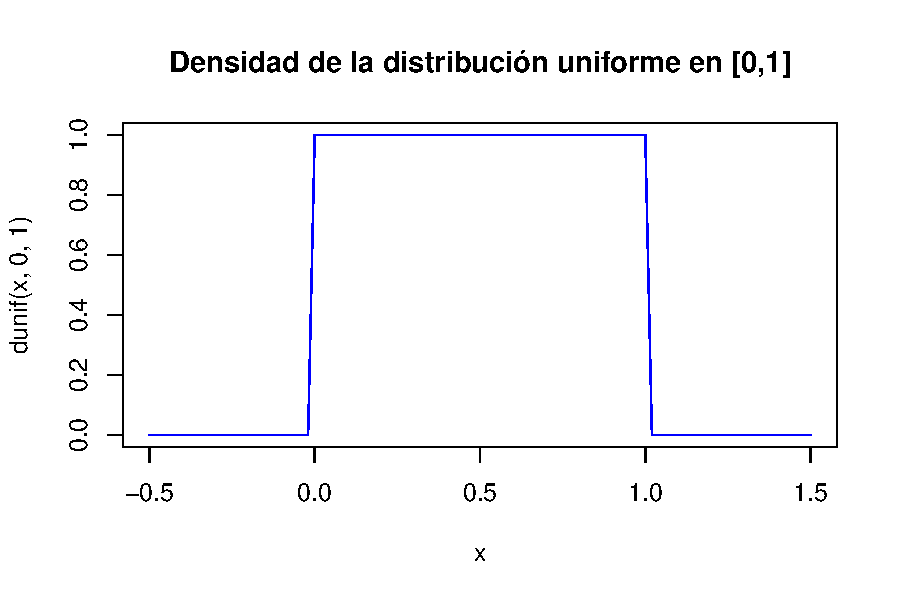
\includegraphics[width=0.5\linewidth,height=\textheight,keepaspectratio]{probabilidad_files/figure-pdf/unnamed-chunk-1-1.pdf}
\end{center}

Por comodidad y conveniencia se opta por representar el espacio muestral
por \[\Omega = \{1,2,3,4,5,6\}.\]

Recordemos la notación \(\mathcal{P}(\Omega)\) que usamos para
referirnos al conjunto de todos los subconjuntos de \(\Omega\). Este
conjunto se llama \textbf{conjunto de partes} de \(\Omega\).

Ejercicio

¿Cuantos elementos contiene el conjunto de partes de \(\Omega\) del
experimento anterior?

Veamos algún ejemplo menos clásico. Podemos considerar el experimento
aleatorio que consiste en calcular los \(n\) gramas de una palabra
escogida al azar.

Ejemplo \(n\)-gramas

Se define un \(n\)-grama de una palabra como el conjunto de \(n\) letras
consecutivas de la misma (contando los blancos de inicio y final de
palabra que marcamos como ``\_'').

Consideremos el experimento aleatorio que consiste en escoger al azar un
3-grama de la palabra ``\_Baleares\_''. Vamos a escribir el espacio
muestral y algunos sucesos elementales del mismo.

En este caso, si consideramos la palabra ``\_Baleares\_'', el espacio
muestral del experimento sería:

\[\Omega=\{\_Ba, Bal, ale, lea, ear, are, res, es\_\}\]

Algunos sucesos serían:

\begin{itemize}
\tightlist
\item
  3-gramas que empiezan por \(a\): \(\{ale,are\}.\)
\item
  3-gramas de inicio y final de palabra: \(\{\_Ba,es\_\}.\)
\item
  3-gramas que contengan una \(l\): \(\{Bal,ale,lea\}.\)
\end{itemize}

Esiten bases de datos que estudián la frecuencias de \(n\)-grams de
caracteres en textos en diferentes idiomas; generalmente de palabras.
Por ejemplo, en español, los bigramas de sílabas más frecuentes son
``EN'' (3.01\%) y ``DE'' (2.77\%) y los trigramas de sílabas son ``QUE''
(1.66\%) y ``ENT'' (1.38\%). Podéis consultar más estadísticas en por
ejemplo en
\href{https://es.sttmedia.com/frecuencias-de-silabas-espanol}{Stefan
Trost Media frecuencias de sílabas en español}.

\subsection{Operaciones con sucesos}\label{operaciones-con-sucesos}

Si tenemos dos sucesos \(A,B\subseteq \Omega\), podemos definir:

\begin{itemize}
\tightlist
\item
  \(\Omega\): \emph{suceso} total o \emph{seguro}.
\item
  \(\emptyset\): suceso \emph{vacío} o \emph{imposible}.
\item
  \(A\cup B\): suceso \emph{unión}; el que ocurre si sucede \(A\) o
  \(B\).
\item
  \(A\cap B\): suceso \emph{intersección}; el que ocurre si sucede \(A\)
  y \(B\).
\item
  \(A^c\): suceso \emph{complementario} el que sucede si NO sucede
  \(A\).
\item
  \(A- B=A\cap B^c\): suceso \emph{diferencia}, que acontece si sucede
  \(A\) y NO sucede \(B\).
\end{itemize}

Sucesos incompatibles

Dos sucesos cualesquiera \(A\) y \(B\) son \emph{incompatibles} (o
\emph{disjuntos}) cuando \(A\cap B=\emptyset\).

Otro ejemplo se observa el sexo y la lateralidad de los estudiantes de
una clase.

Ejemplo

Supongamos que el sexo se divide entre Mujeres y Hombres y la
lateralirad en diestros y zurdos. Vamos a definir el espacio muestral,
los sucesos elementales y a realizar algunas operaciones entre ellos.

Estudiantes de esta clase: \(\Omega\). - Mujeres de esta clase: \(A\). -
Estudiantes que son zurdos \(B\).

Algunas operaciones entre los sucesos anteriores serían:

\begin{itemize}
\tightlist
\item
  \(A\cup B\): Est. que son mujeres o que son zurdos.
\item
  \(A\cap B\): Mujeres de esta clase que son zurdas.
\item
  \(A^c\): Hombres de esta clase.
\item
  \(A-B\): Mujeres de la clases que NO son zurdas.
\item
  \(B-A\): Hombres de la clase que son zurdos.
\item
  ¡Cuidado! No son incompatibles.
\end{itemize}

\subsection{Propiedades}\label{propiedades}

Propiedades

\textbf{Conmutativas}:

\[A\cup B=B\cup A, \quad A\cap B=B\cap A\]

\textbf{Asociativas}:

\begin{align*}
A\cup(B\cup C)=(A\cup B)\cup C, \\
A\cap(B\cap C)=(A\cap B)\cap C.
\end{align*}

\textbf{Distributivas}

\begin{align*}
A\cap & (B\cup C)=(A\cap B)\cup (A\cap C),\\ 
A\cup & (B\cap C)=(A\cup B)\cap (A\cup C).
\end{align*}

Veamos algunos diagramas que nos ayuda a demostrar las propiedades
anteriores.

\begin{longtable}[]{@{}
  >{\centering\arraybackslash}p{(\linewidth - 4\tabcolsep) * \real{0.3333}}
  >{\centering\arraybackslash}p{(\linewidth - 4\tabcolsep) * \real{0.3333}}
  >{\centering\arraybackslash}p{(\linewidth - 4\tabcolsep) * \real{0.3333}}@{}}
\toprule\noalign{}
\begin{minipage}[b]{\linewidth}\centering
\(A\)
\end{minipage} & \begin{minipage}[b]{\linewidth}\centering
\(B\cap C\)
\end{minipage} & \begin{minipage}[b]{\linewidth}\centering
\(A\cup (B\cap C)\)
\end{minipage} \\
\midrule\noalign{}
\endhead
\bottomrule\noalign{}
\endlastfoot
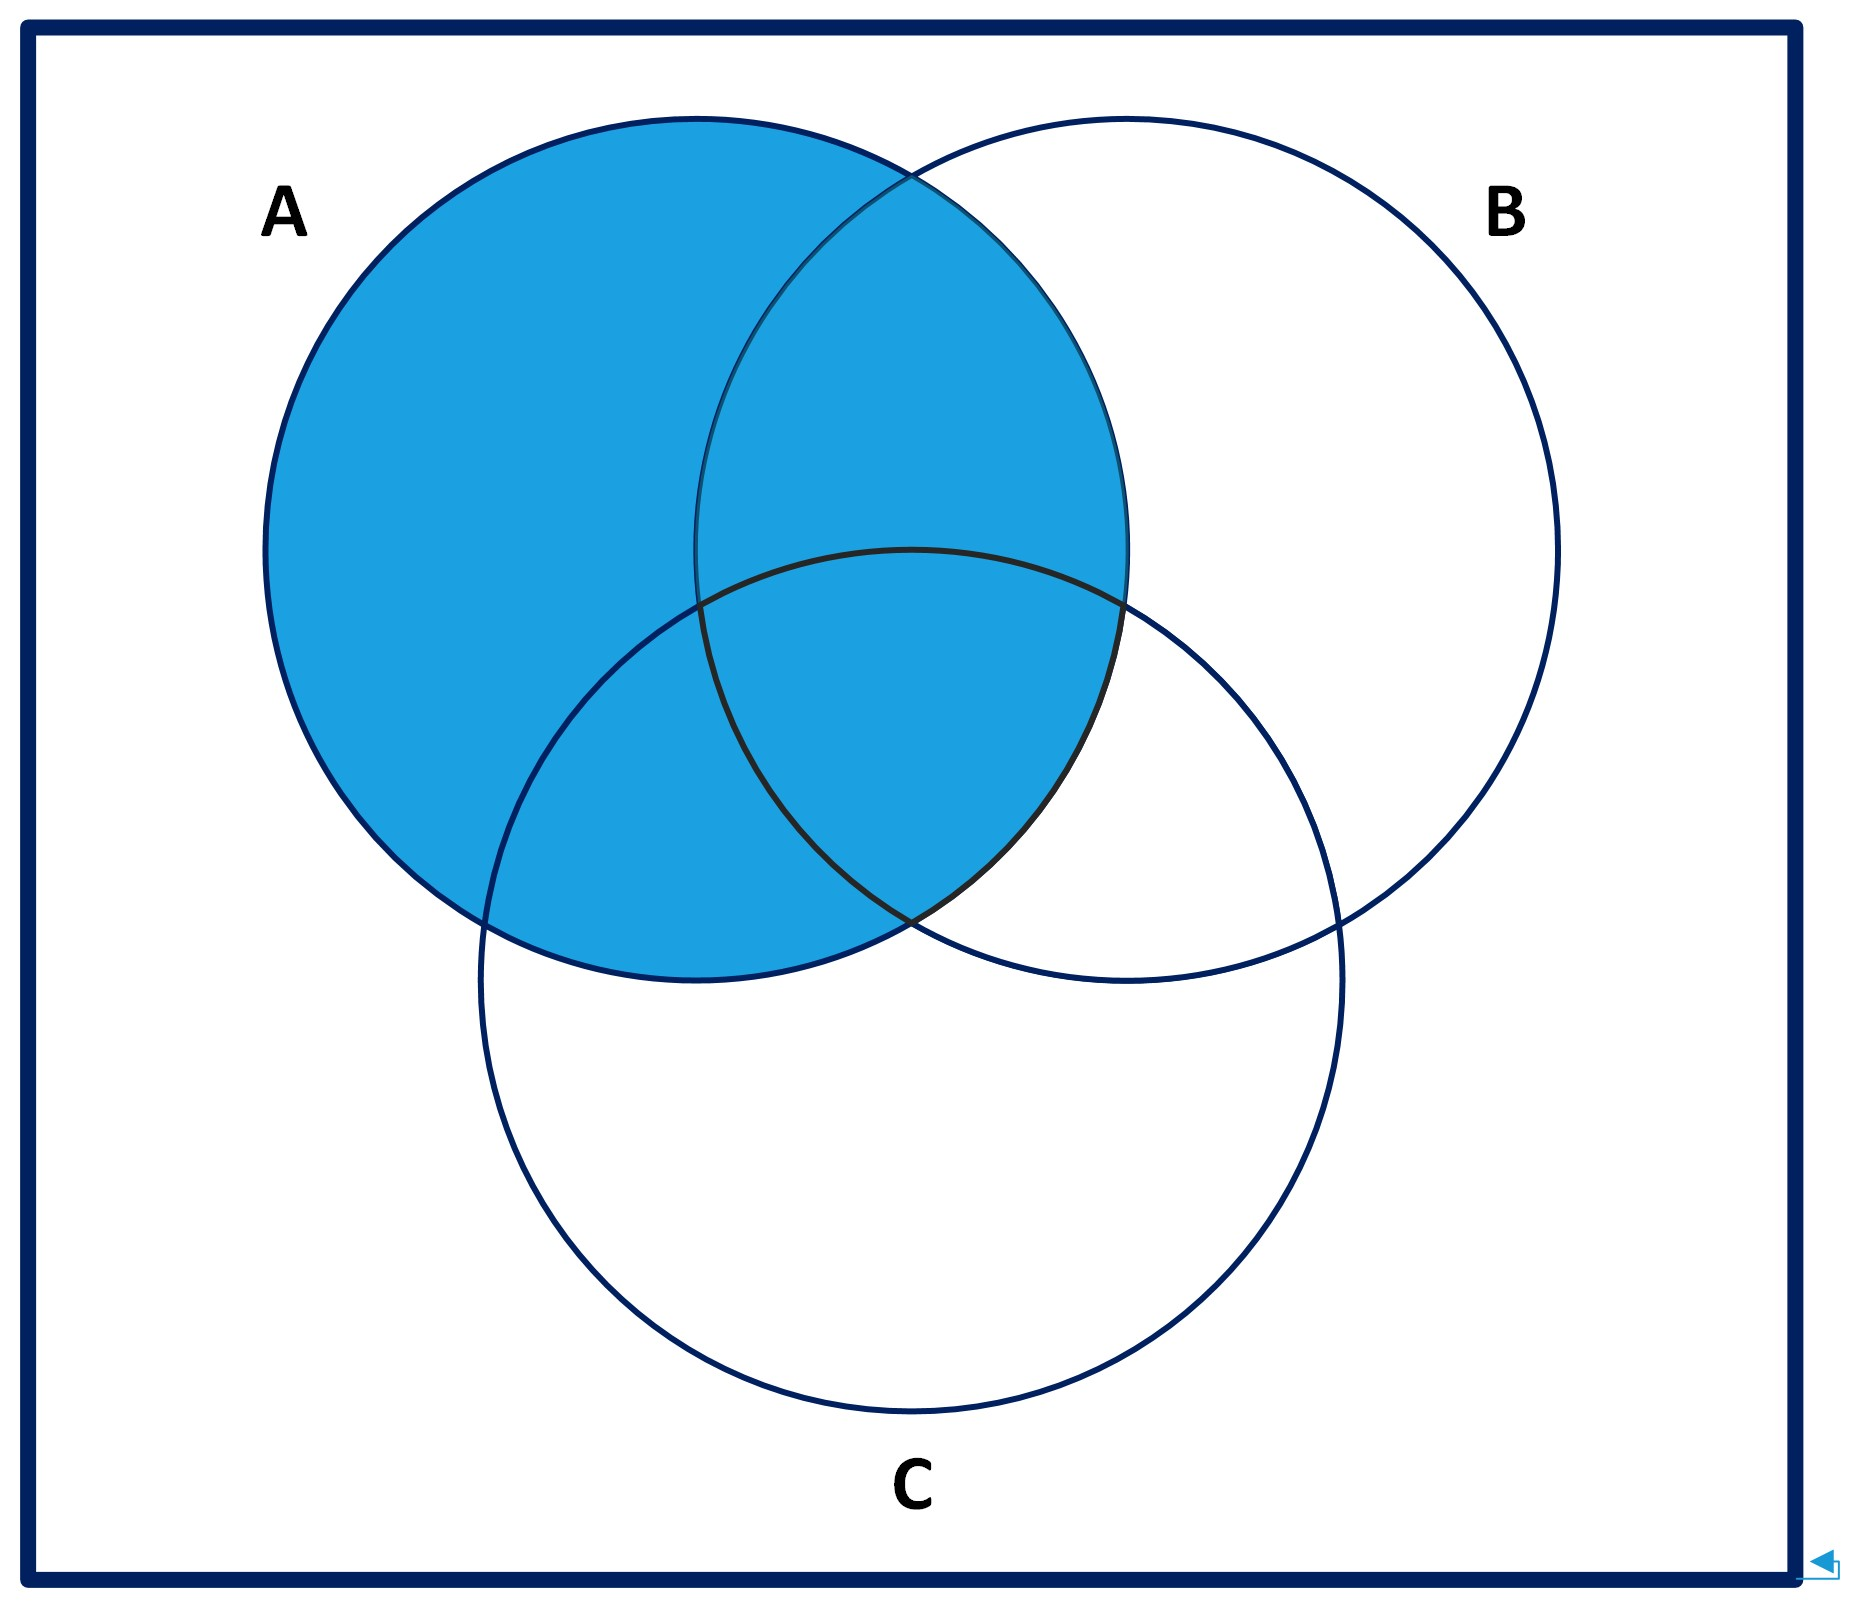
\includegraphics[width=\linewidth,height=1.5625in,keepaspectratio]{Images/venn1A.jpeg}
&
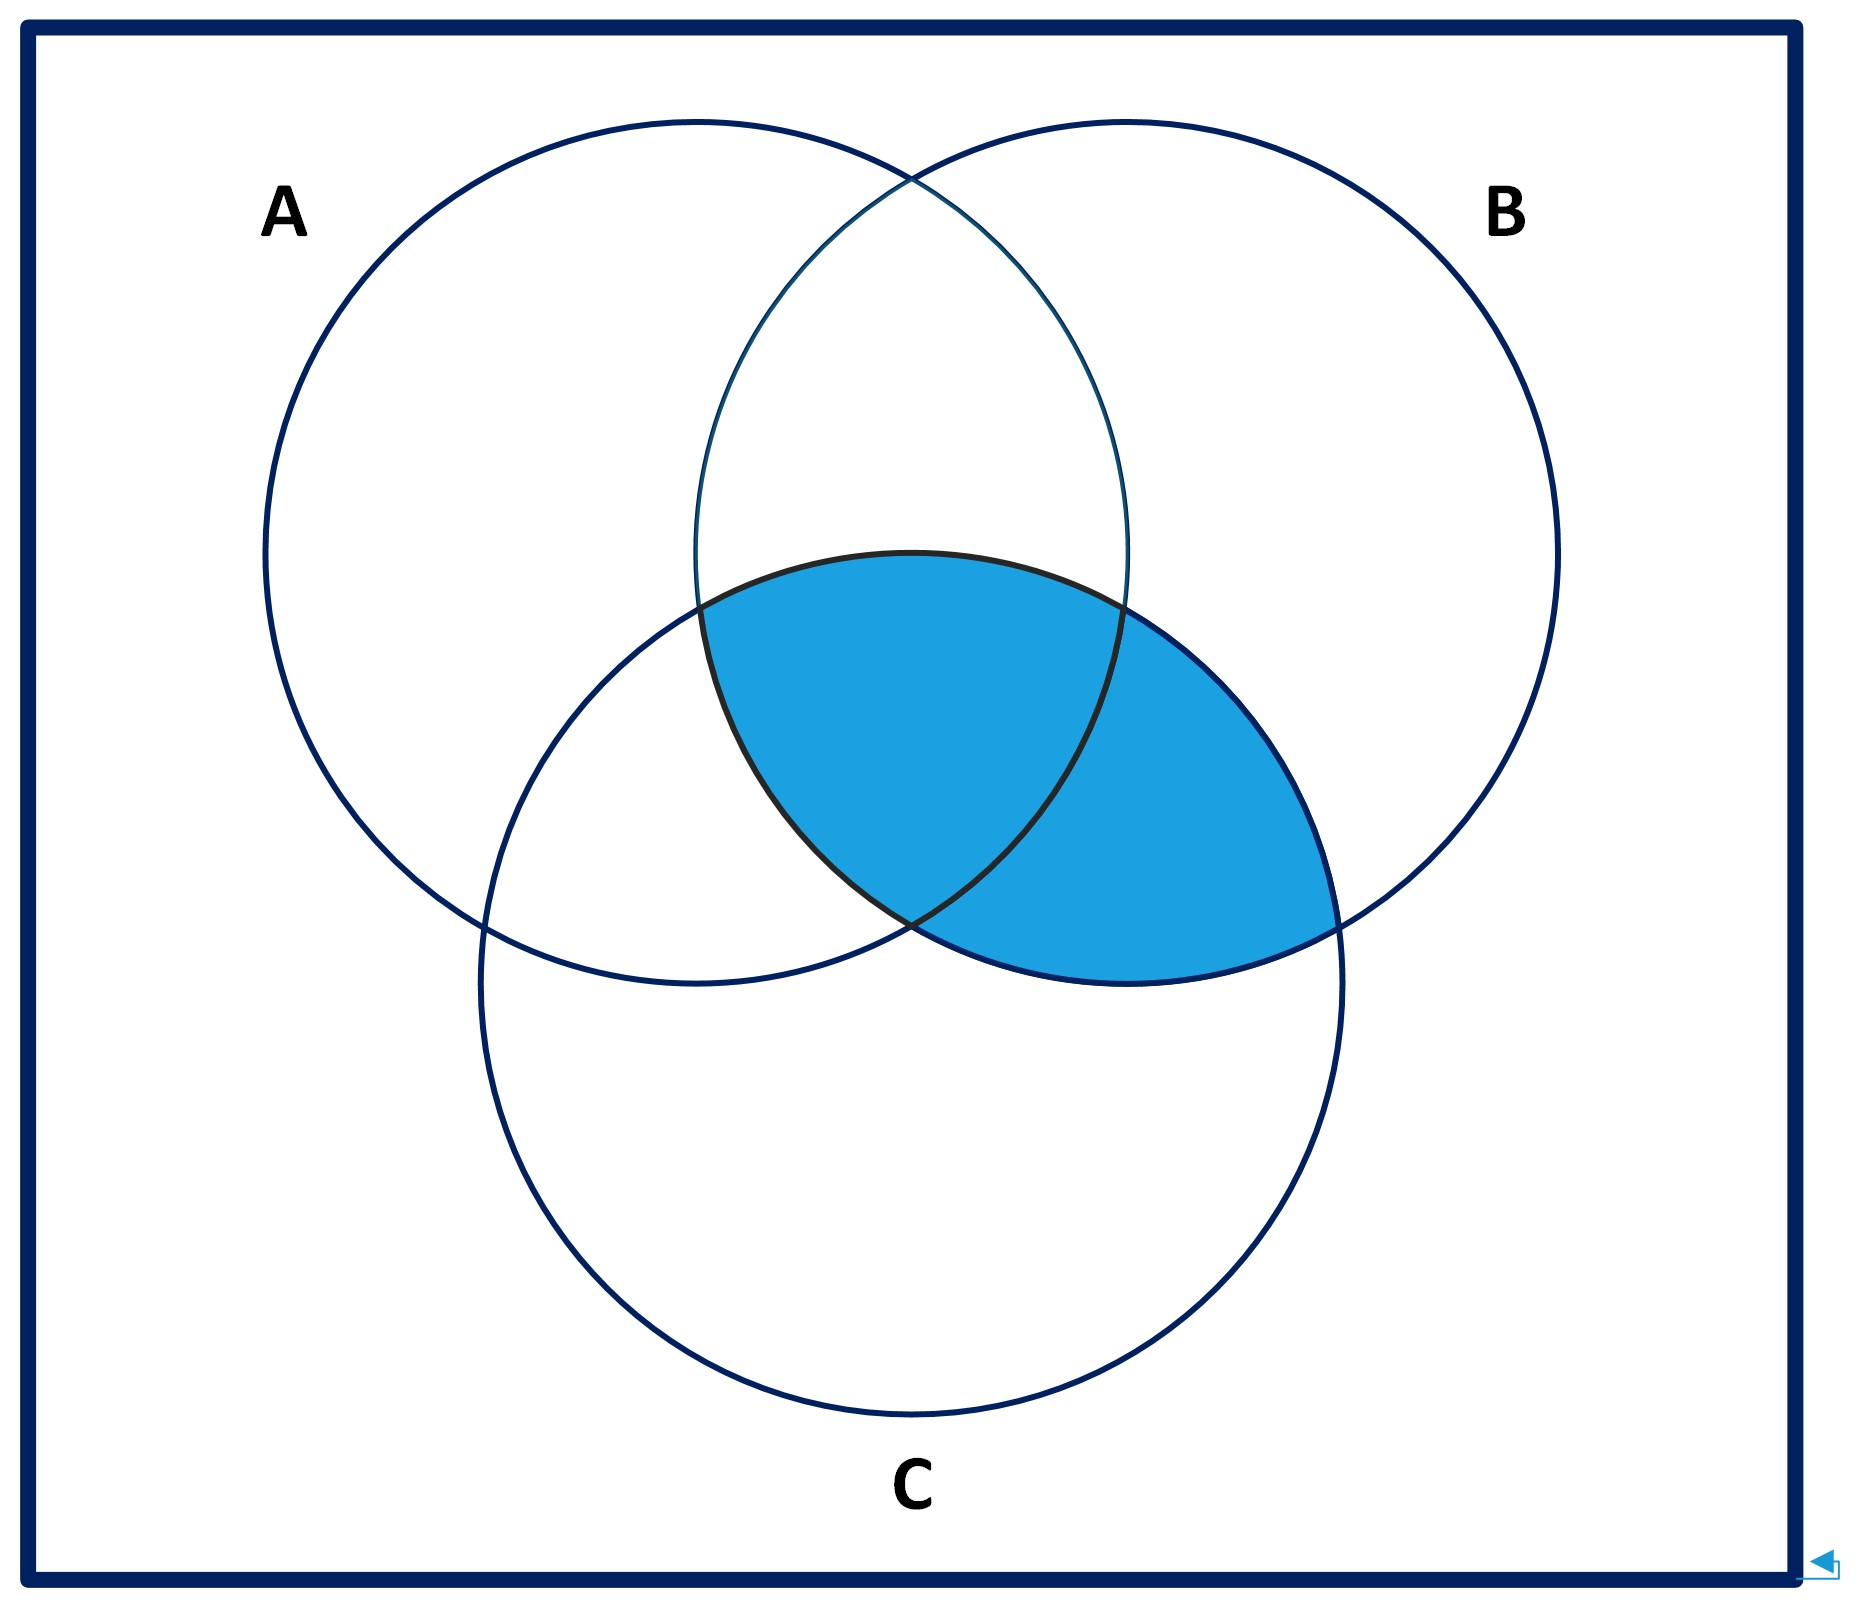
\includegraphics[width=\linewidth,height=1.5625in,keepaspectratio]{Images/venn1ByC.jpeg}
&
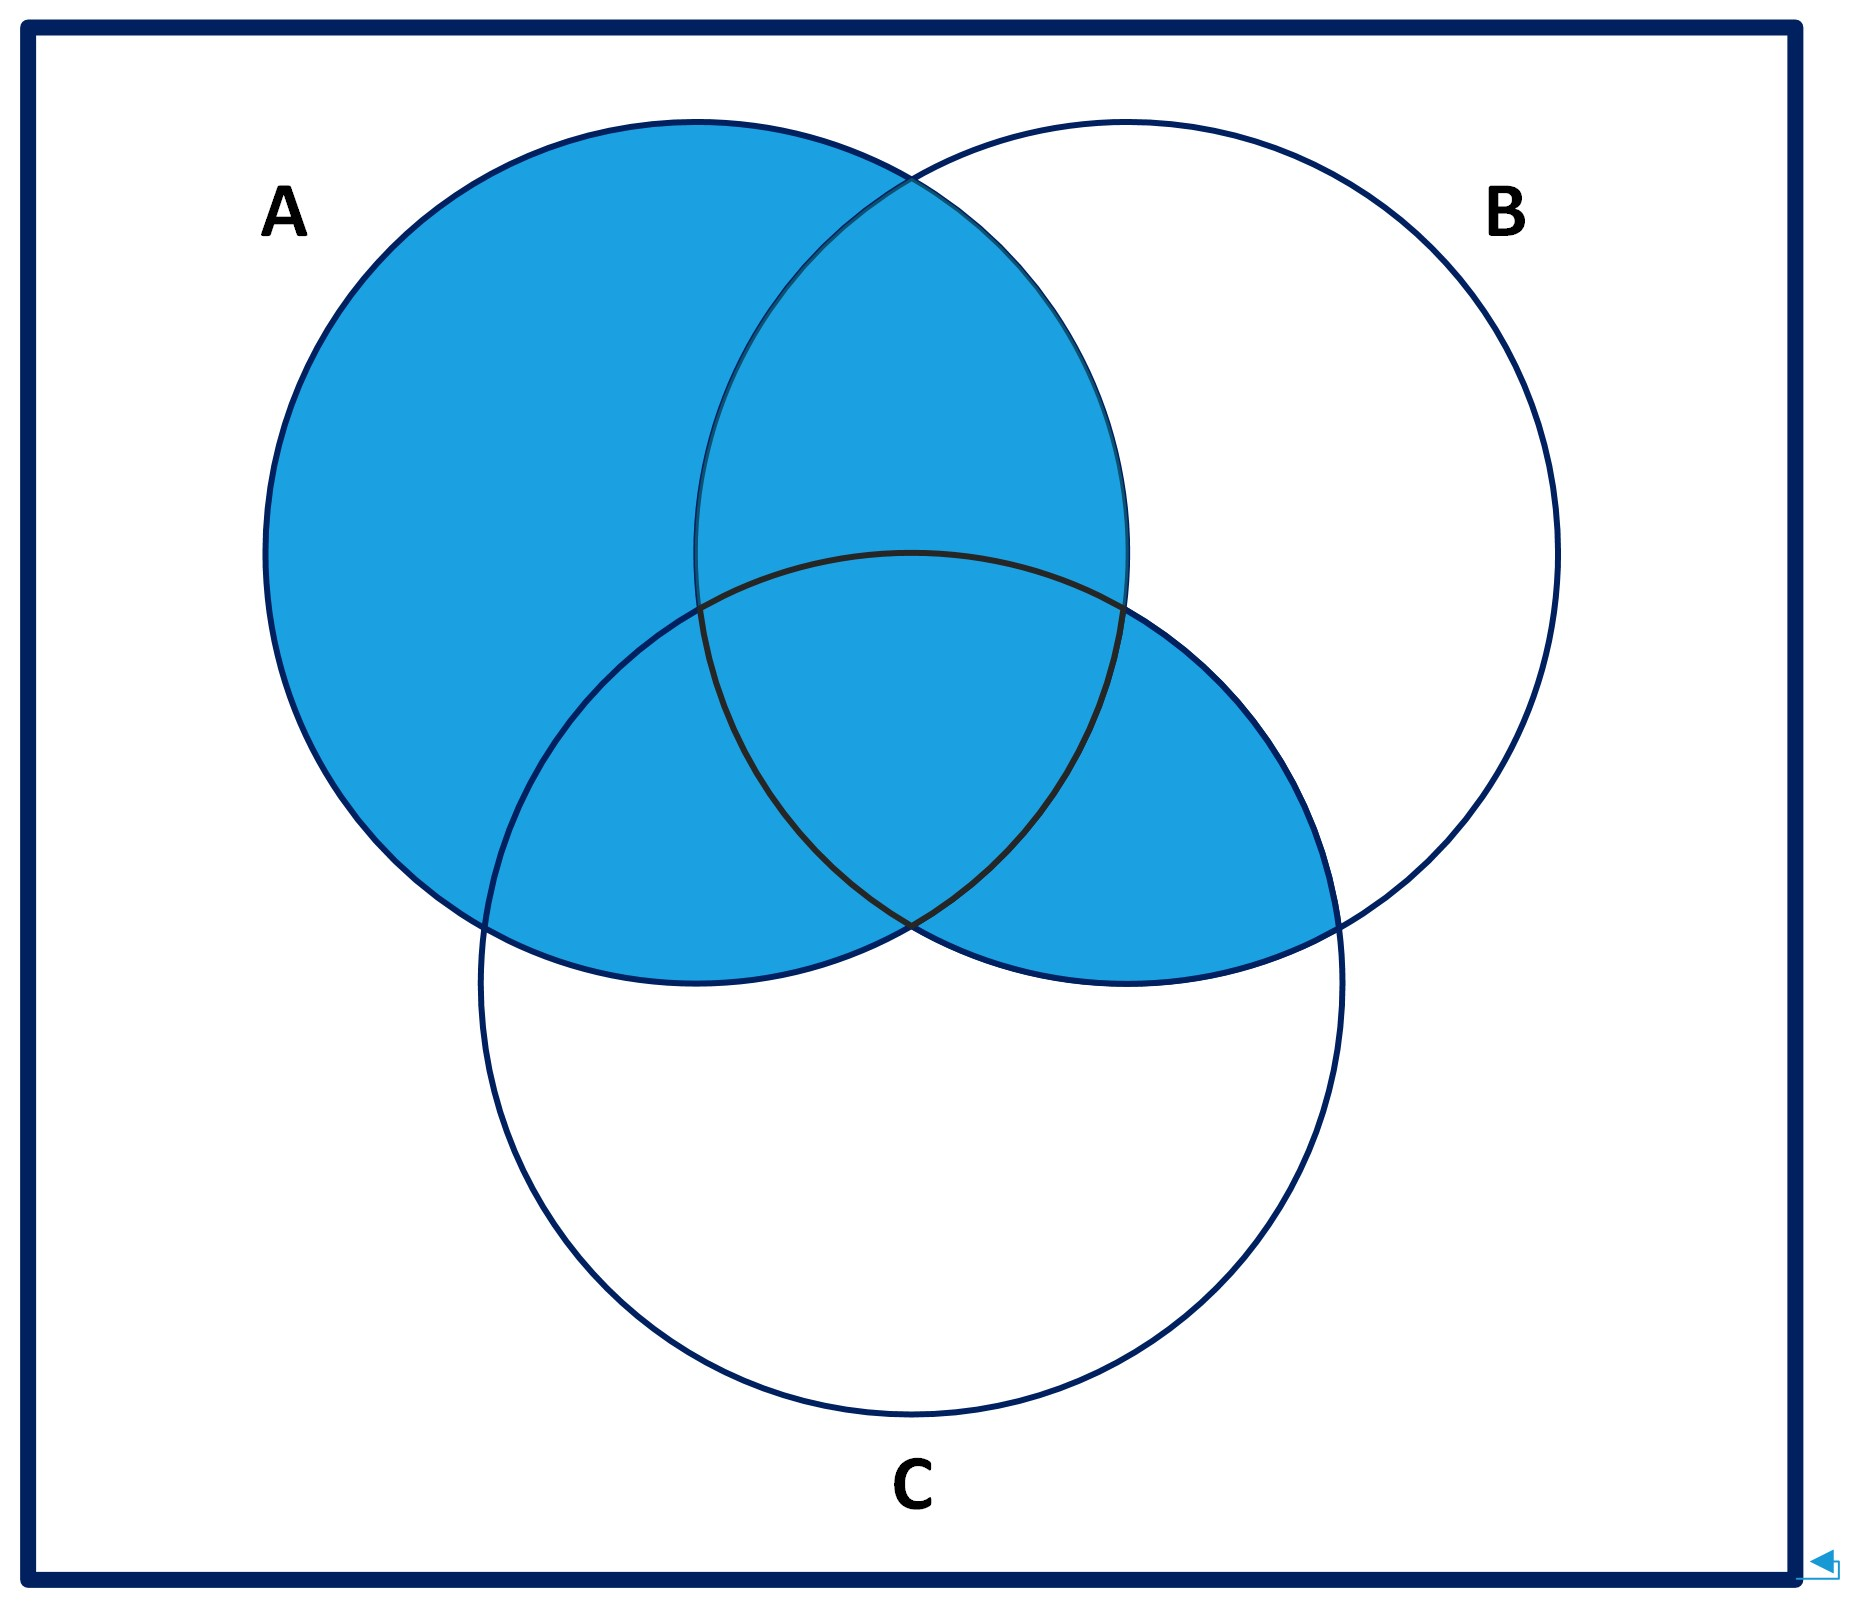
\includegraphics[width=\linewidth,height=1.5625in,keepaspectratio]{Images/venn1AUByC.jpeg} \\
\end{longtable}

\begin{longtable}[]{@{}
  >{\centering\arraybackslash}p{(\linewidth - 4\tabcolsep) * \real{0.3333}}
  >{\centering\arraybackslash}p{(\linewidth - 4\tabcolsep) * \real{0.3333}}
  >{\centering\arraybackslash}p{(\linewidth - 4\tabcolsep) * \real{0.3333}}@{}}
\toprule\noalign{}
\begin{minipage}[b]{\linewidth}\centering
\(A\cup B\)
\end{minipage} & \begin{minipage}[b]{\linewidth}\centering
\(A\cup C\)
\end{minipage} & \begin{minipage}[b]{\linewidth}\centering
\((A\cup B)\cap (A\cup C)\)
\end{minipage} \\
\midrule\noalign{}
\endhead
\bottomrule\noalign{}
\endlastfoot
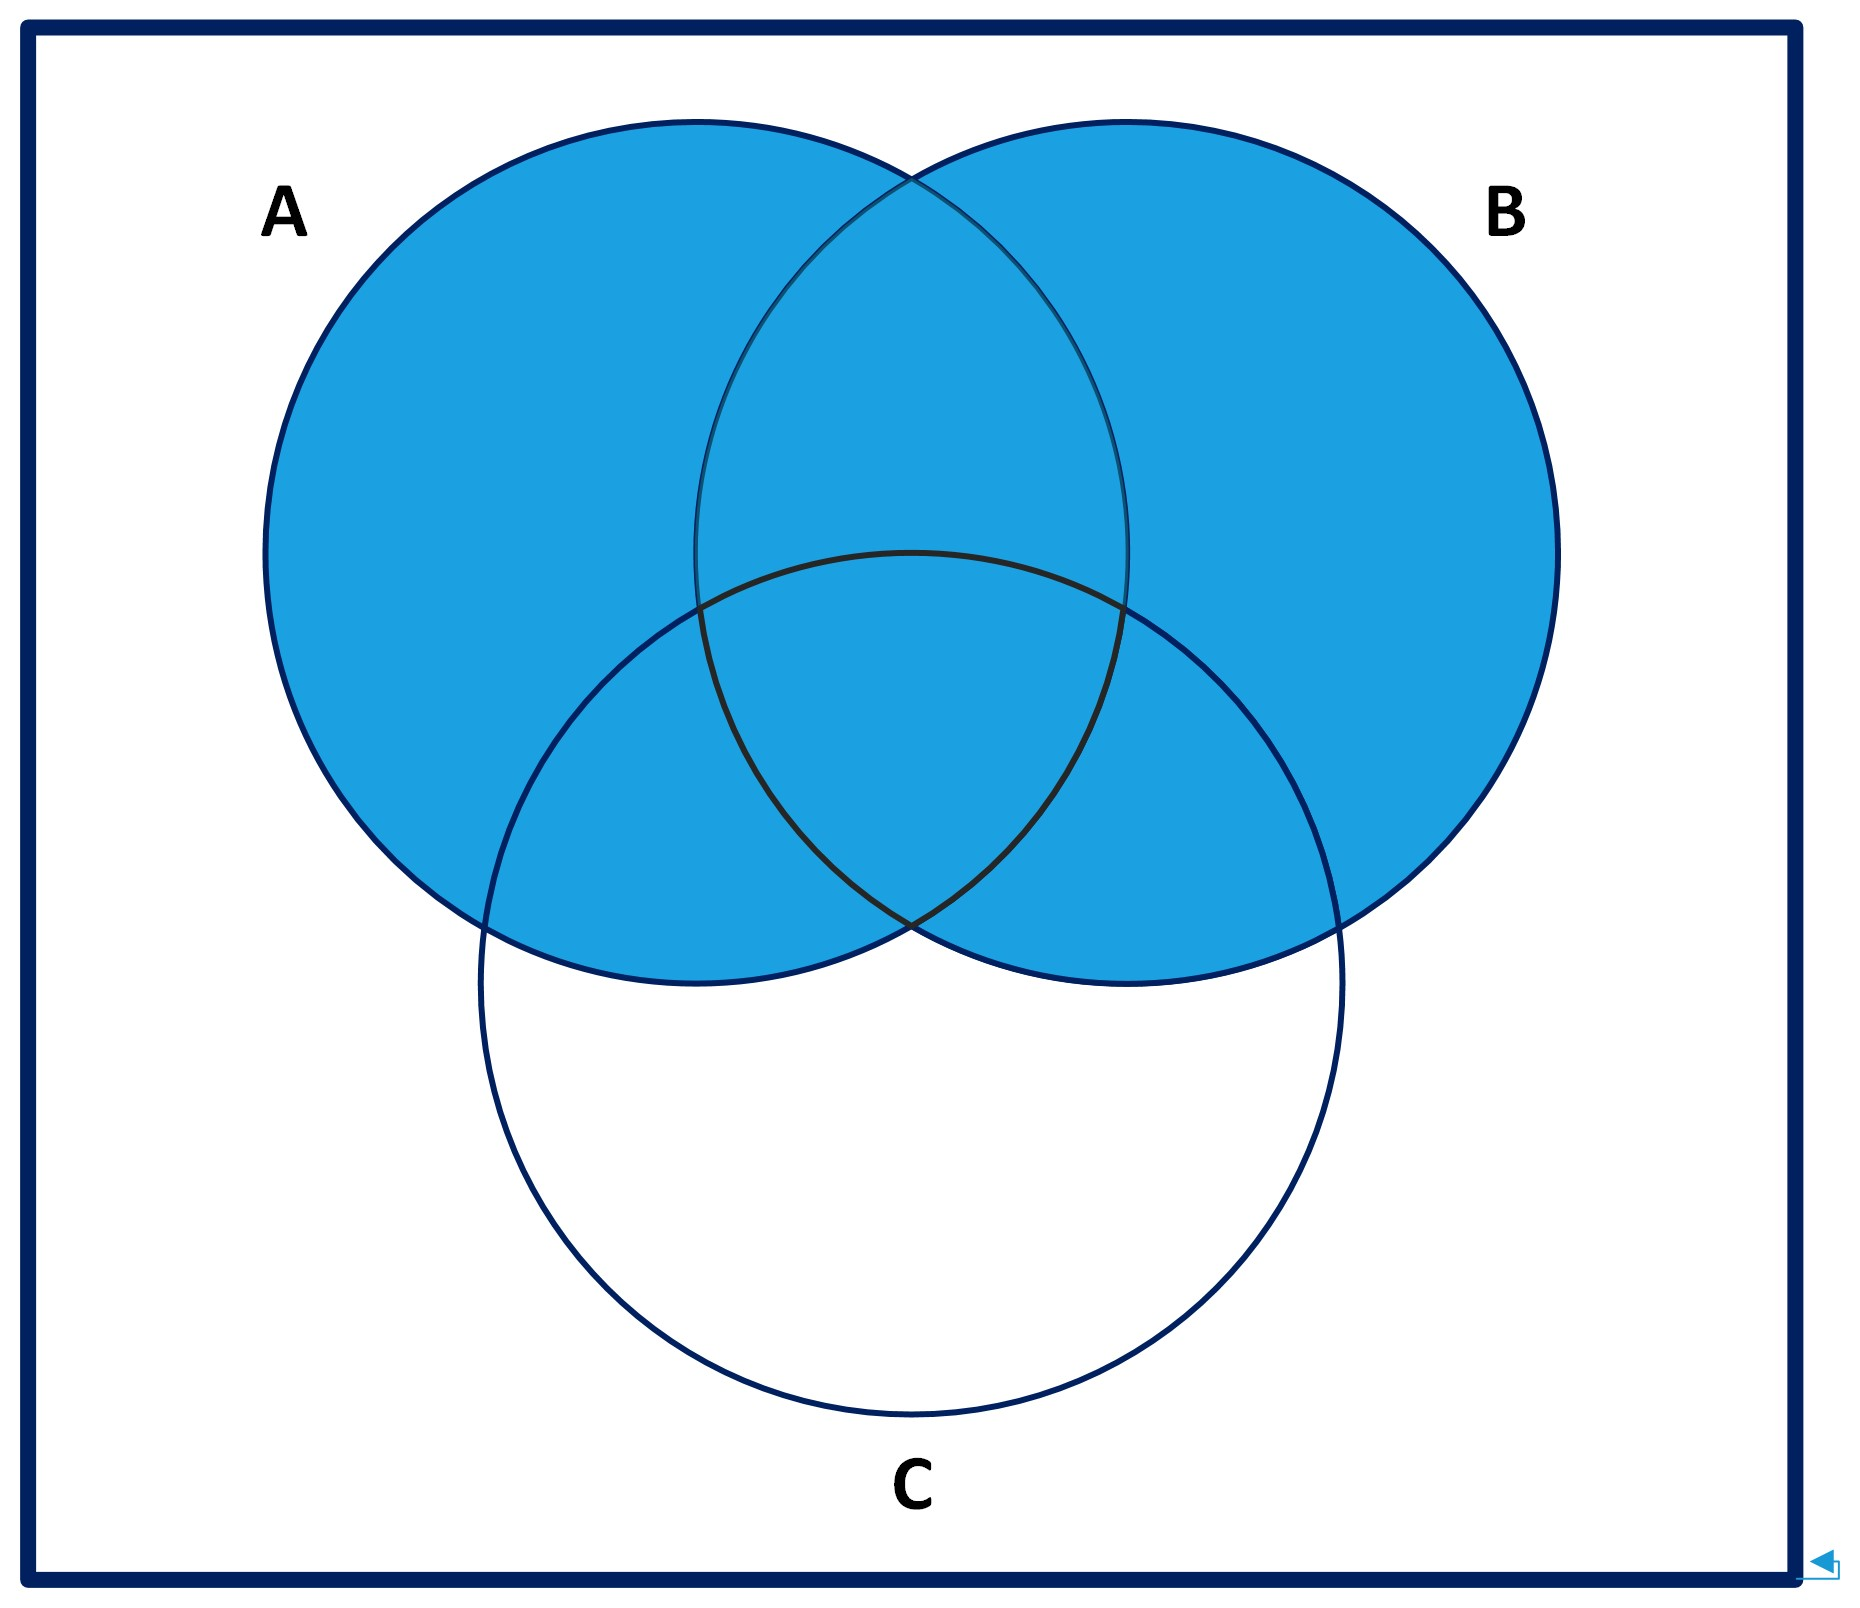
\includegraphics[width=\linewidth,height=1.5625in,keepaspectratio]{Images/venn1AoB.jpeg}
&
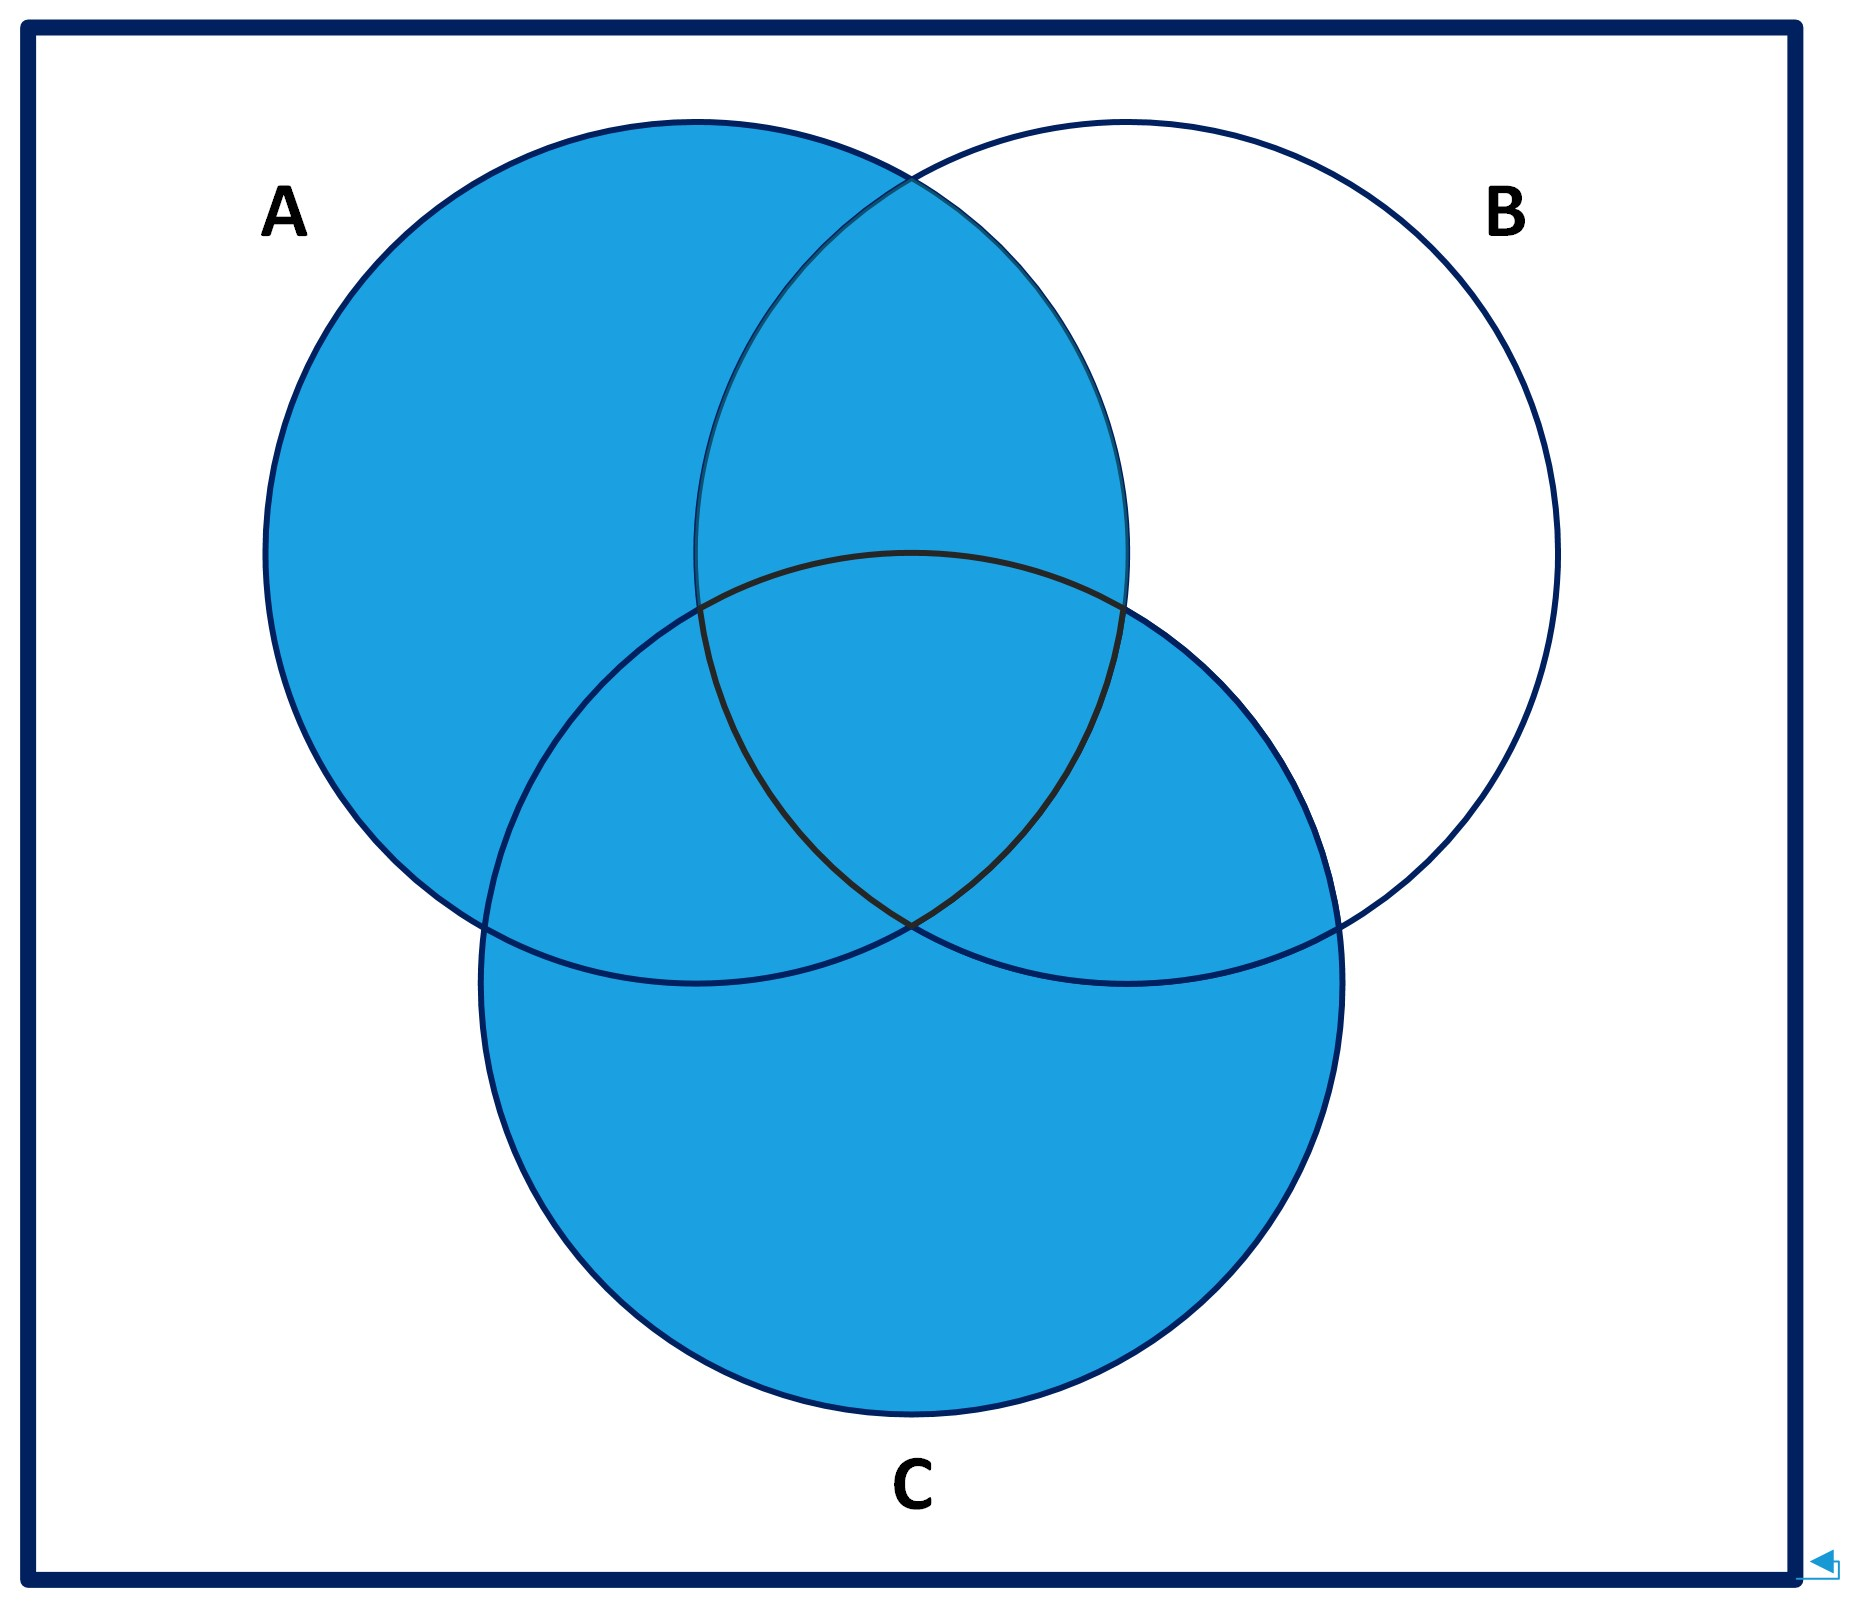
\includegraphics[width=\linewidth,height=1.5625in,keepaspectratio]{Images/venn1AoC.jpeg}
&
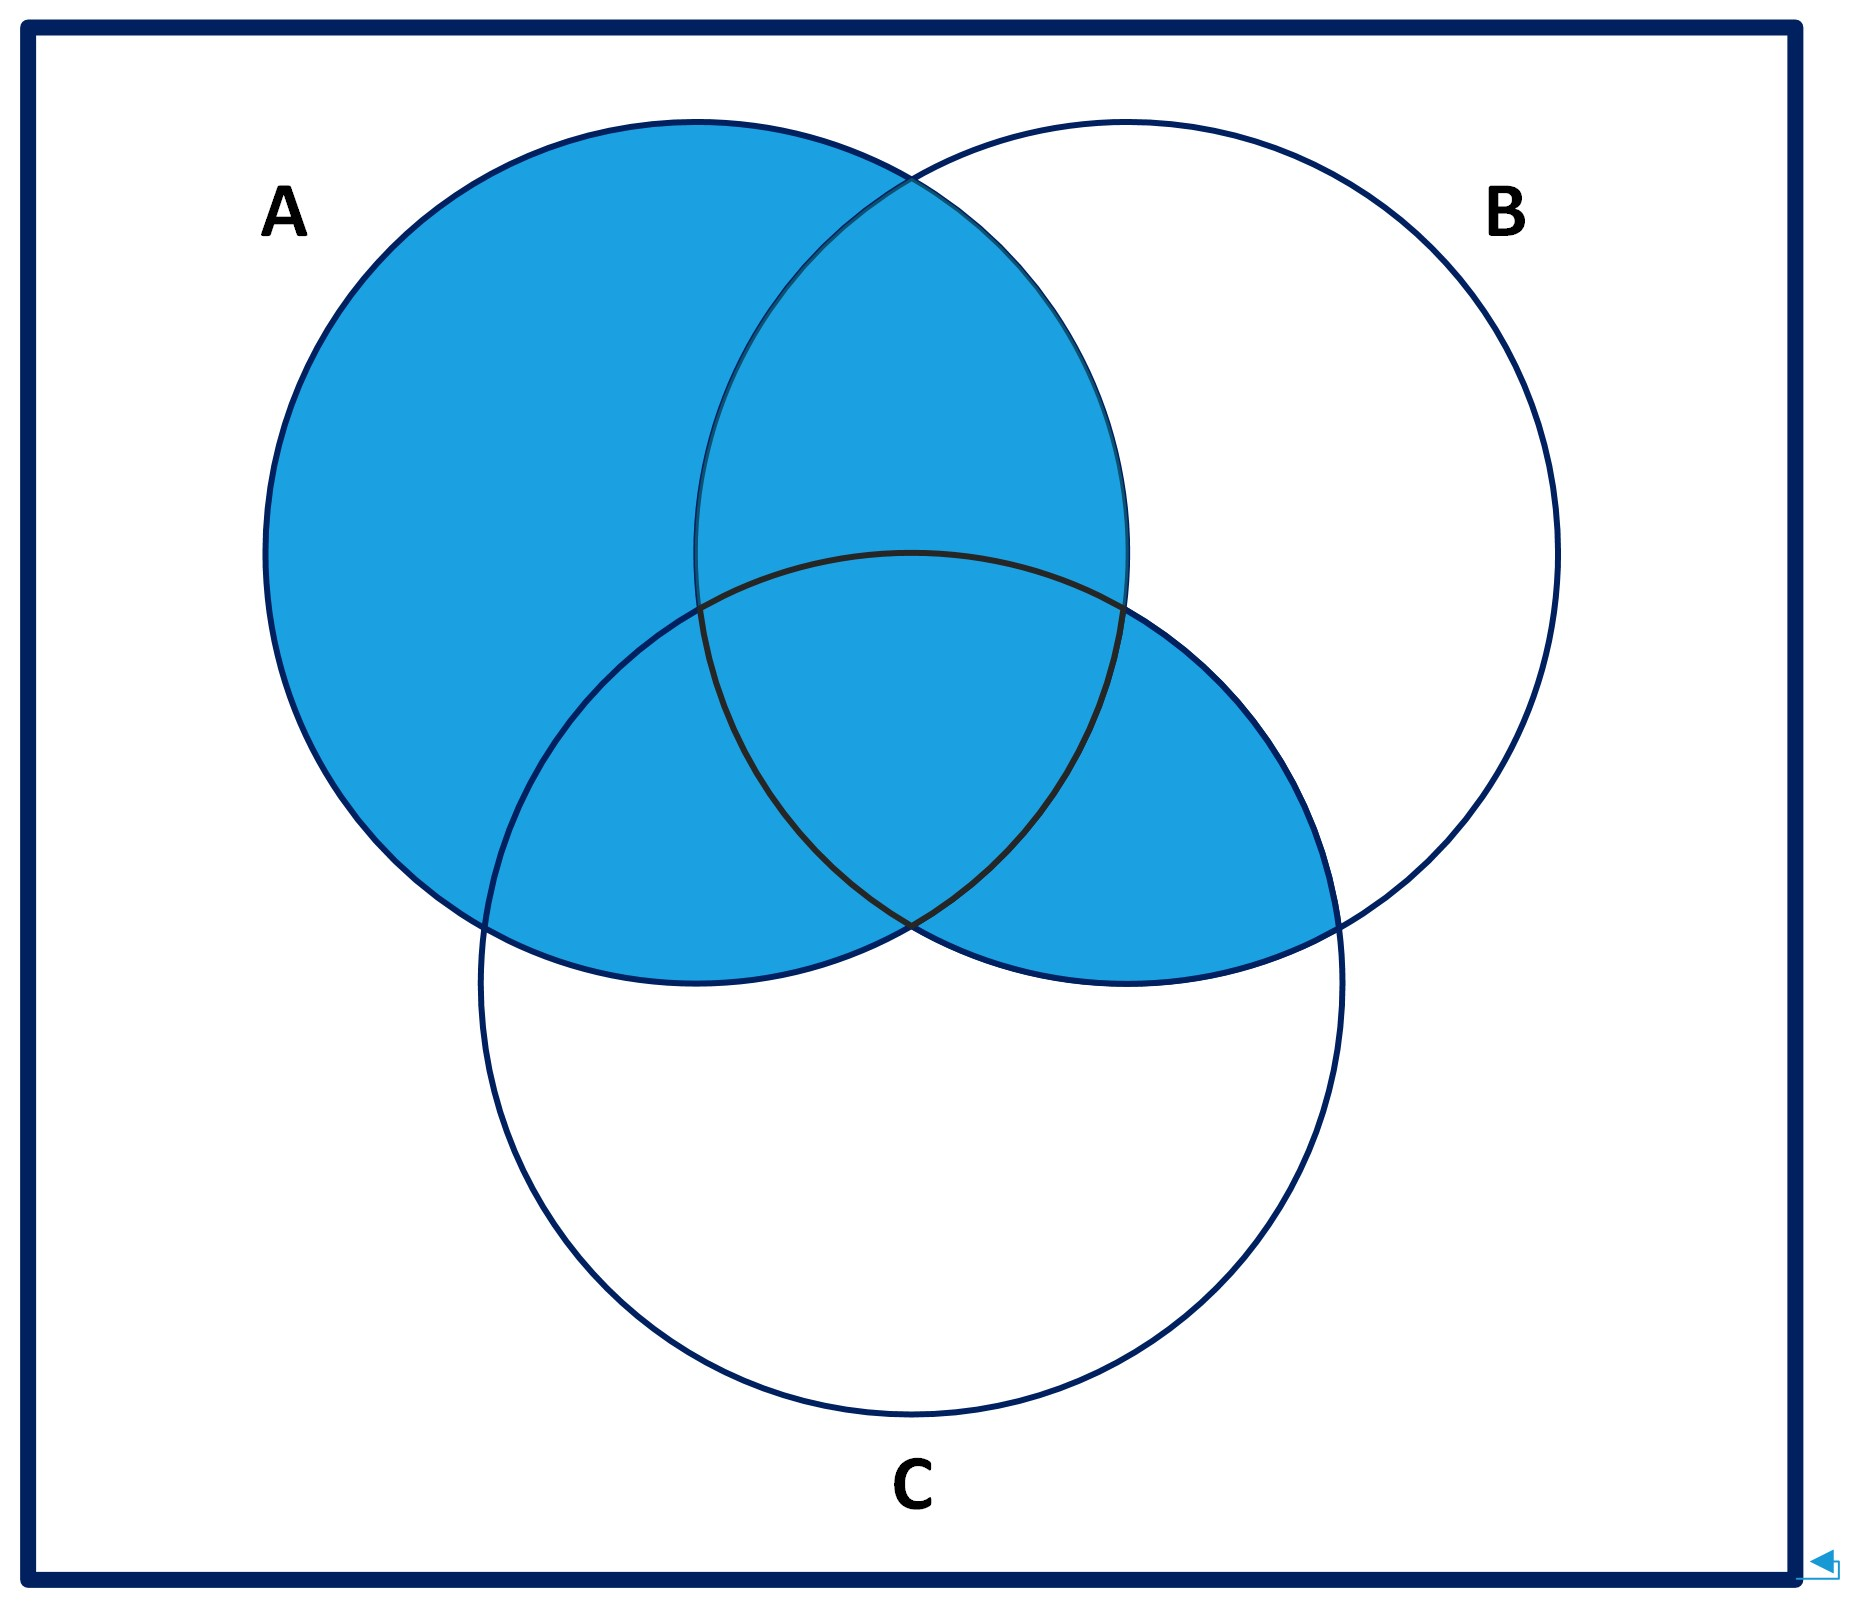
\includegraphics[width=\linewidth,height=1.5625in,keepaspectratio]{Images/venn1AUByC.jpeg} \\
\end{longtable}

Complementario del complementario

\[(A^c)^c=A\]

\begin{longtable}[]{@{}
  >{\centering\arraybackslash}p{(\linewidth - 4\tabcolsep) * \real{0.3333}}
  >{\centering\arraybackslash}p{(\linewidth - 4\tabcolsep) * \real{0.3333}}
  >{\centering\arraybackslash}p{(\linewidth - 4\tabcolsep) * \real{0.3333}}@{}}
\toprule\noalign{}
\begin{minipage}[b]{\linewidth}\centering
\(A\)
\end{minipage} & \begin{minipage}[b]{\linewidth}\centering
\(A^c\)
\end{minipage} & \begin{minipage}[b]{\linewidth}\centering
\((A^c)^c\)
\end{minipage} \\
\midrule\noalign{}
\endhead
\bottomrule\noalign{}
\endlastfoot
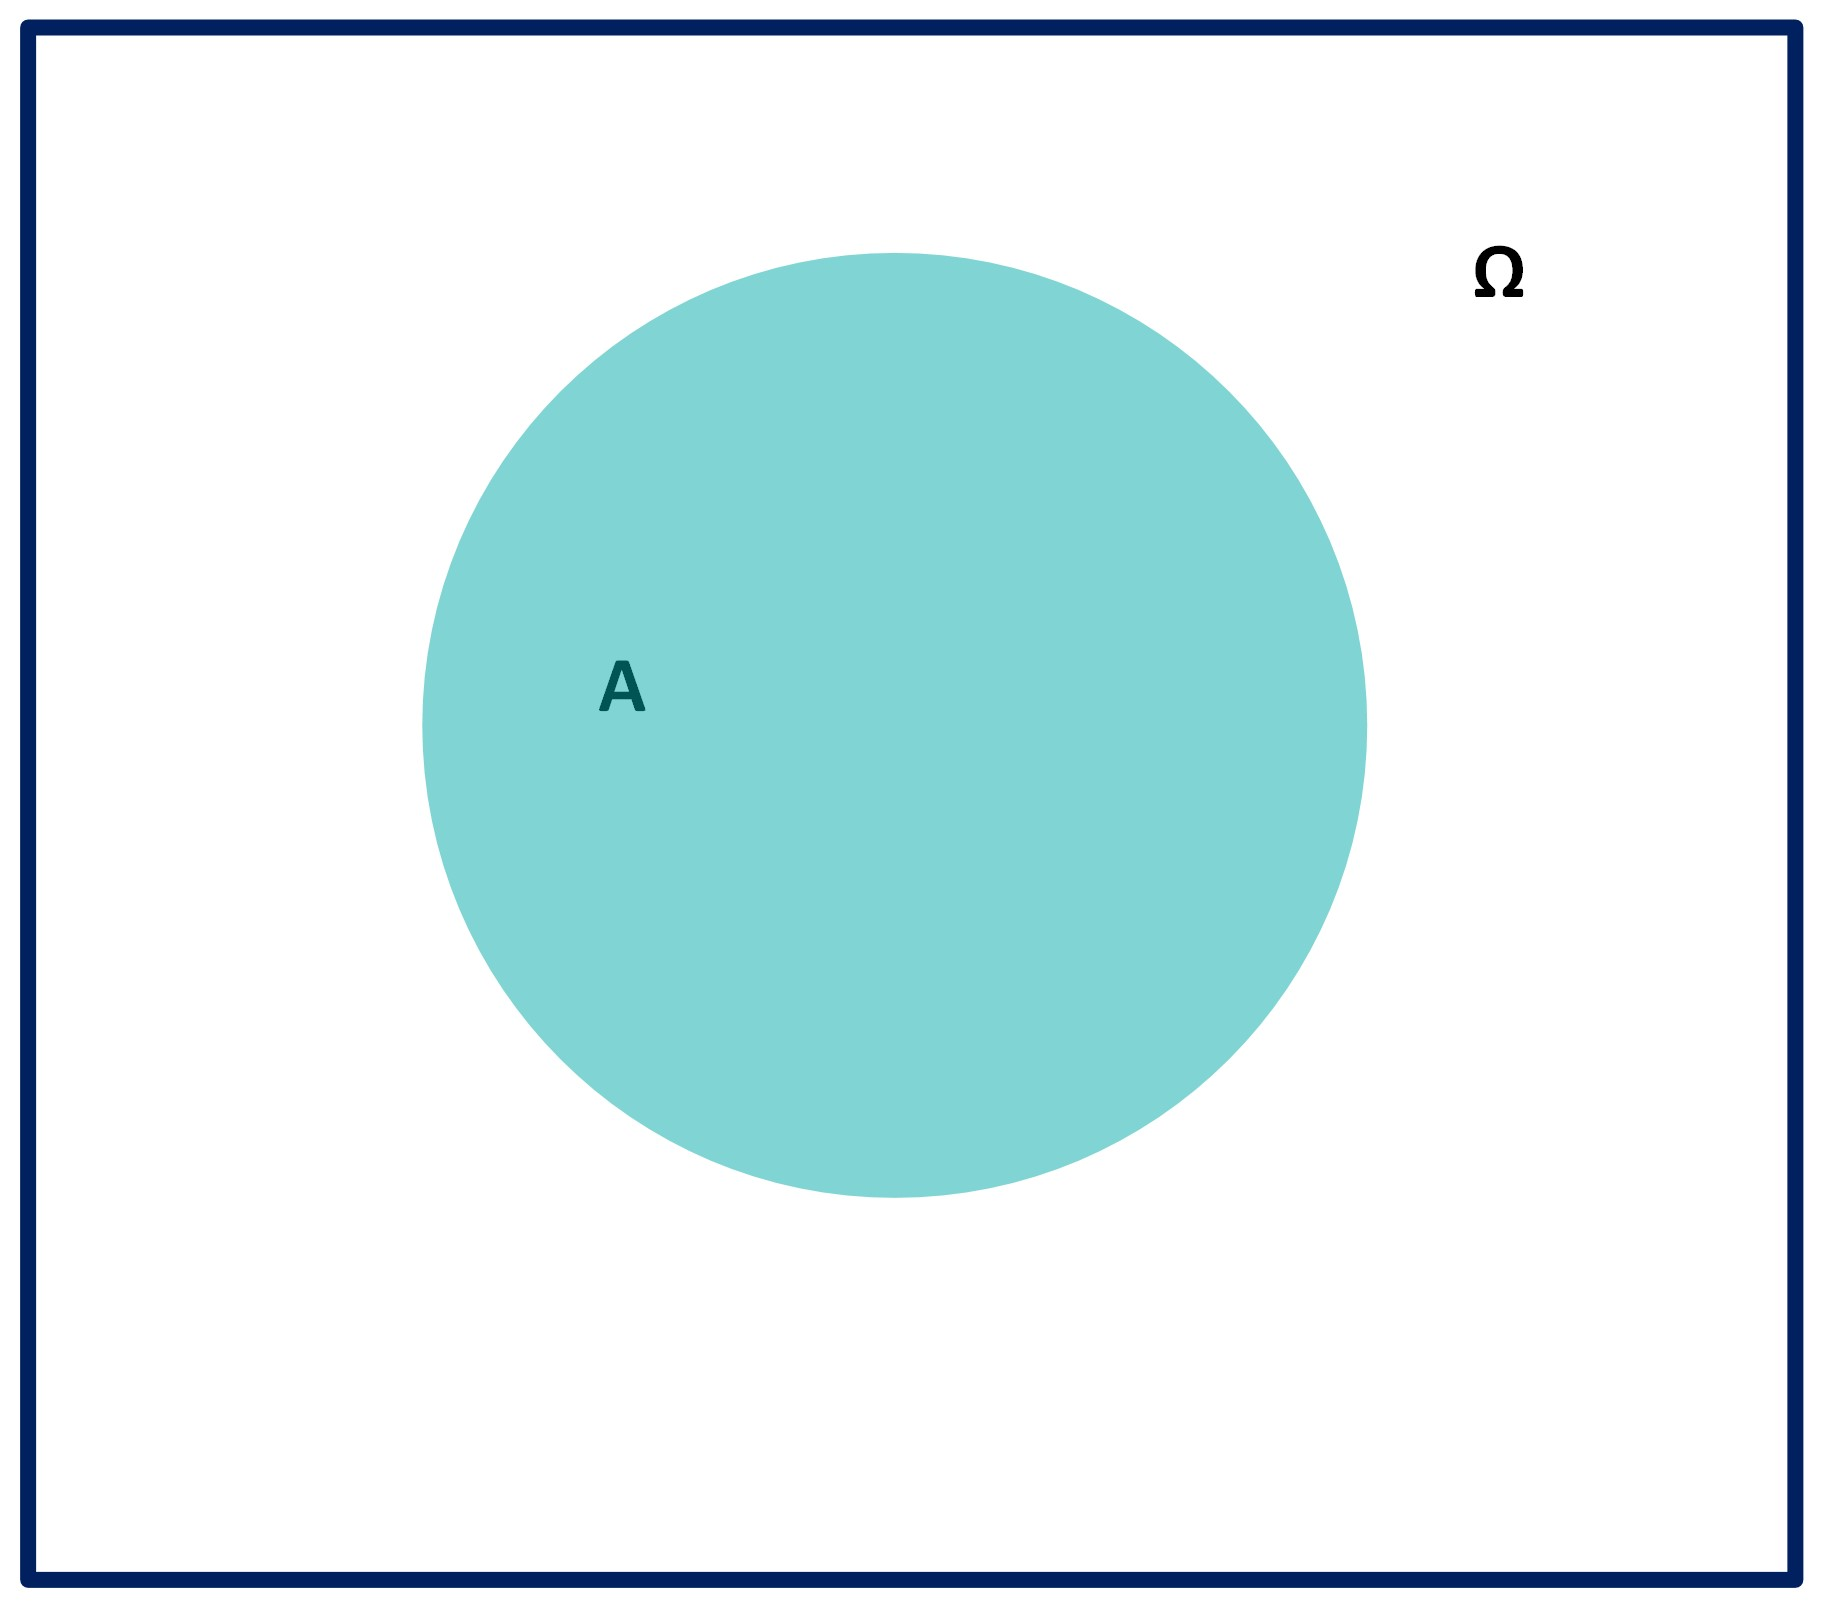
\includegraphics[width=\linewidth,height=1.5625in,keepaspectratio]{Images/venn1A_solo.jpeg}
&
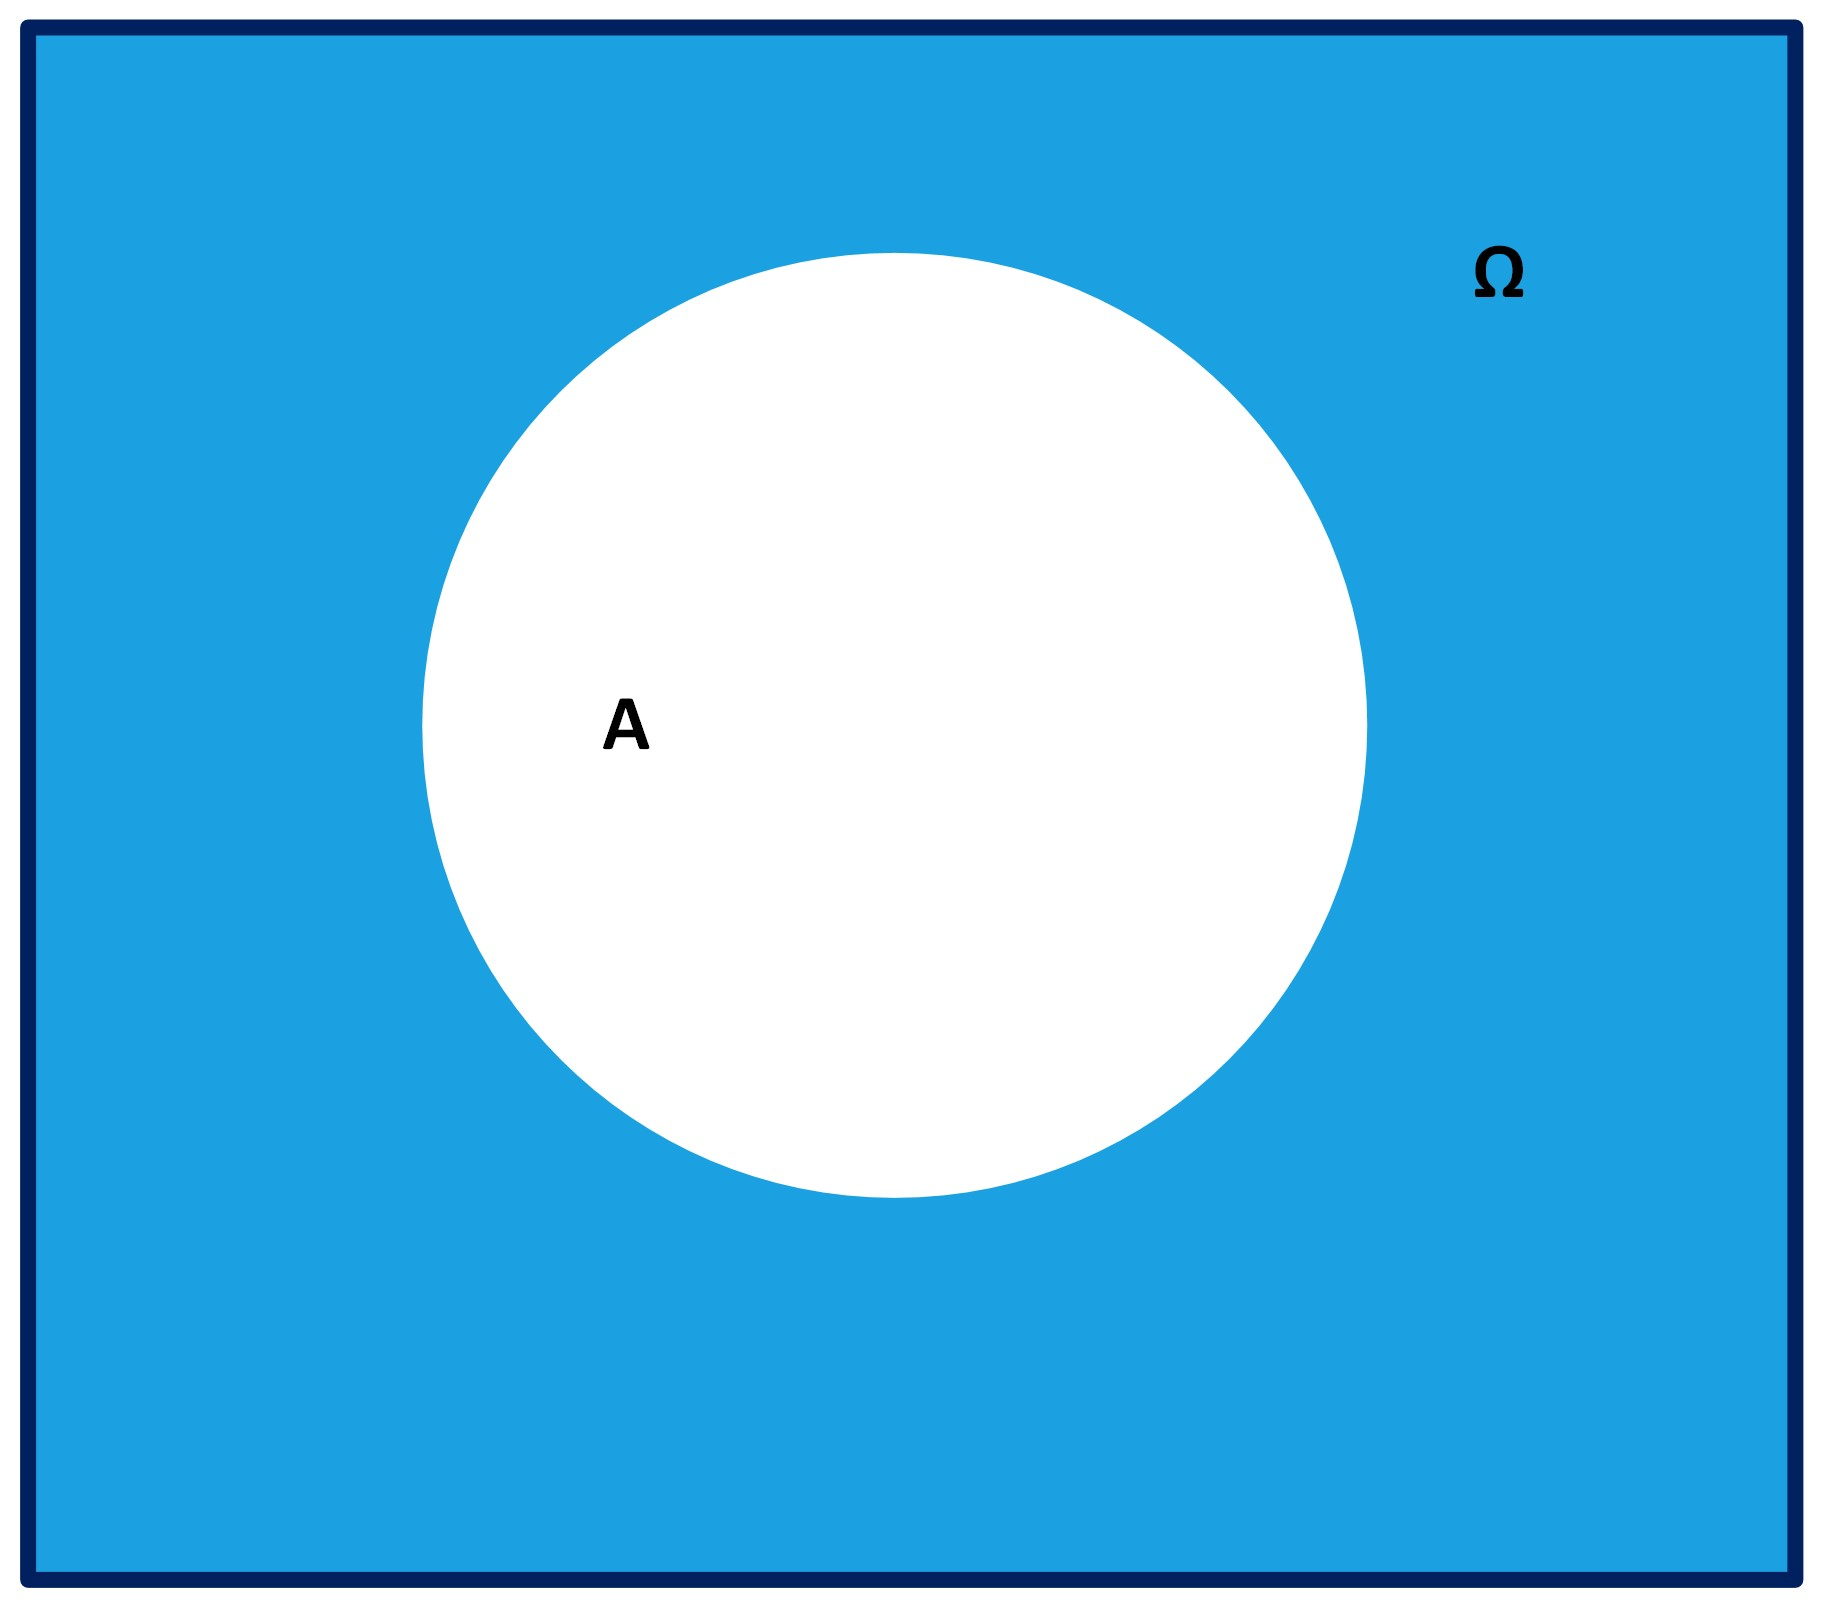
\includegraphics[width=\linewidth,height=1.5625in,keepaspectratio]{Images/venn1solo_Ac.jpeg}
&
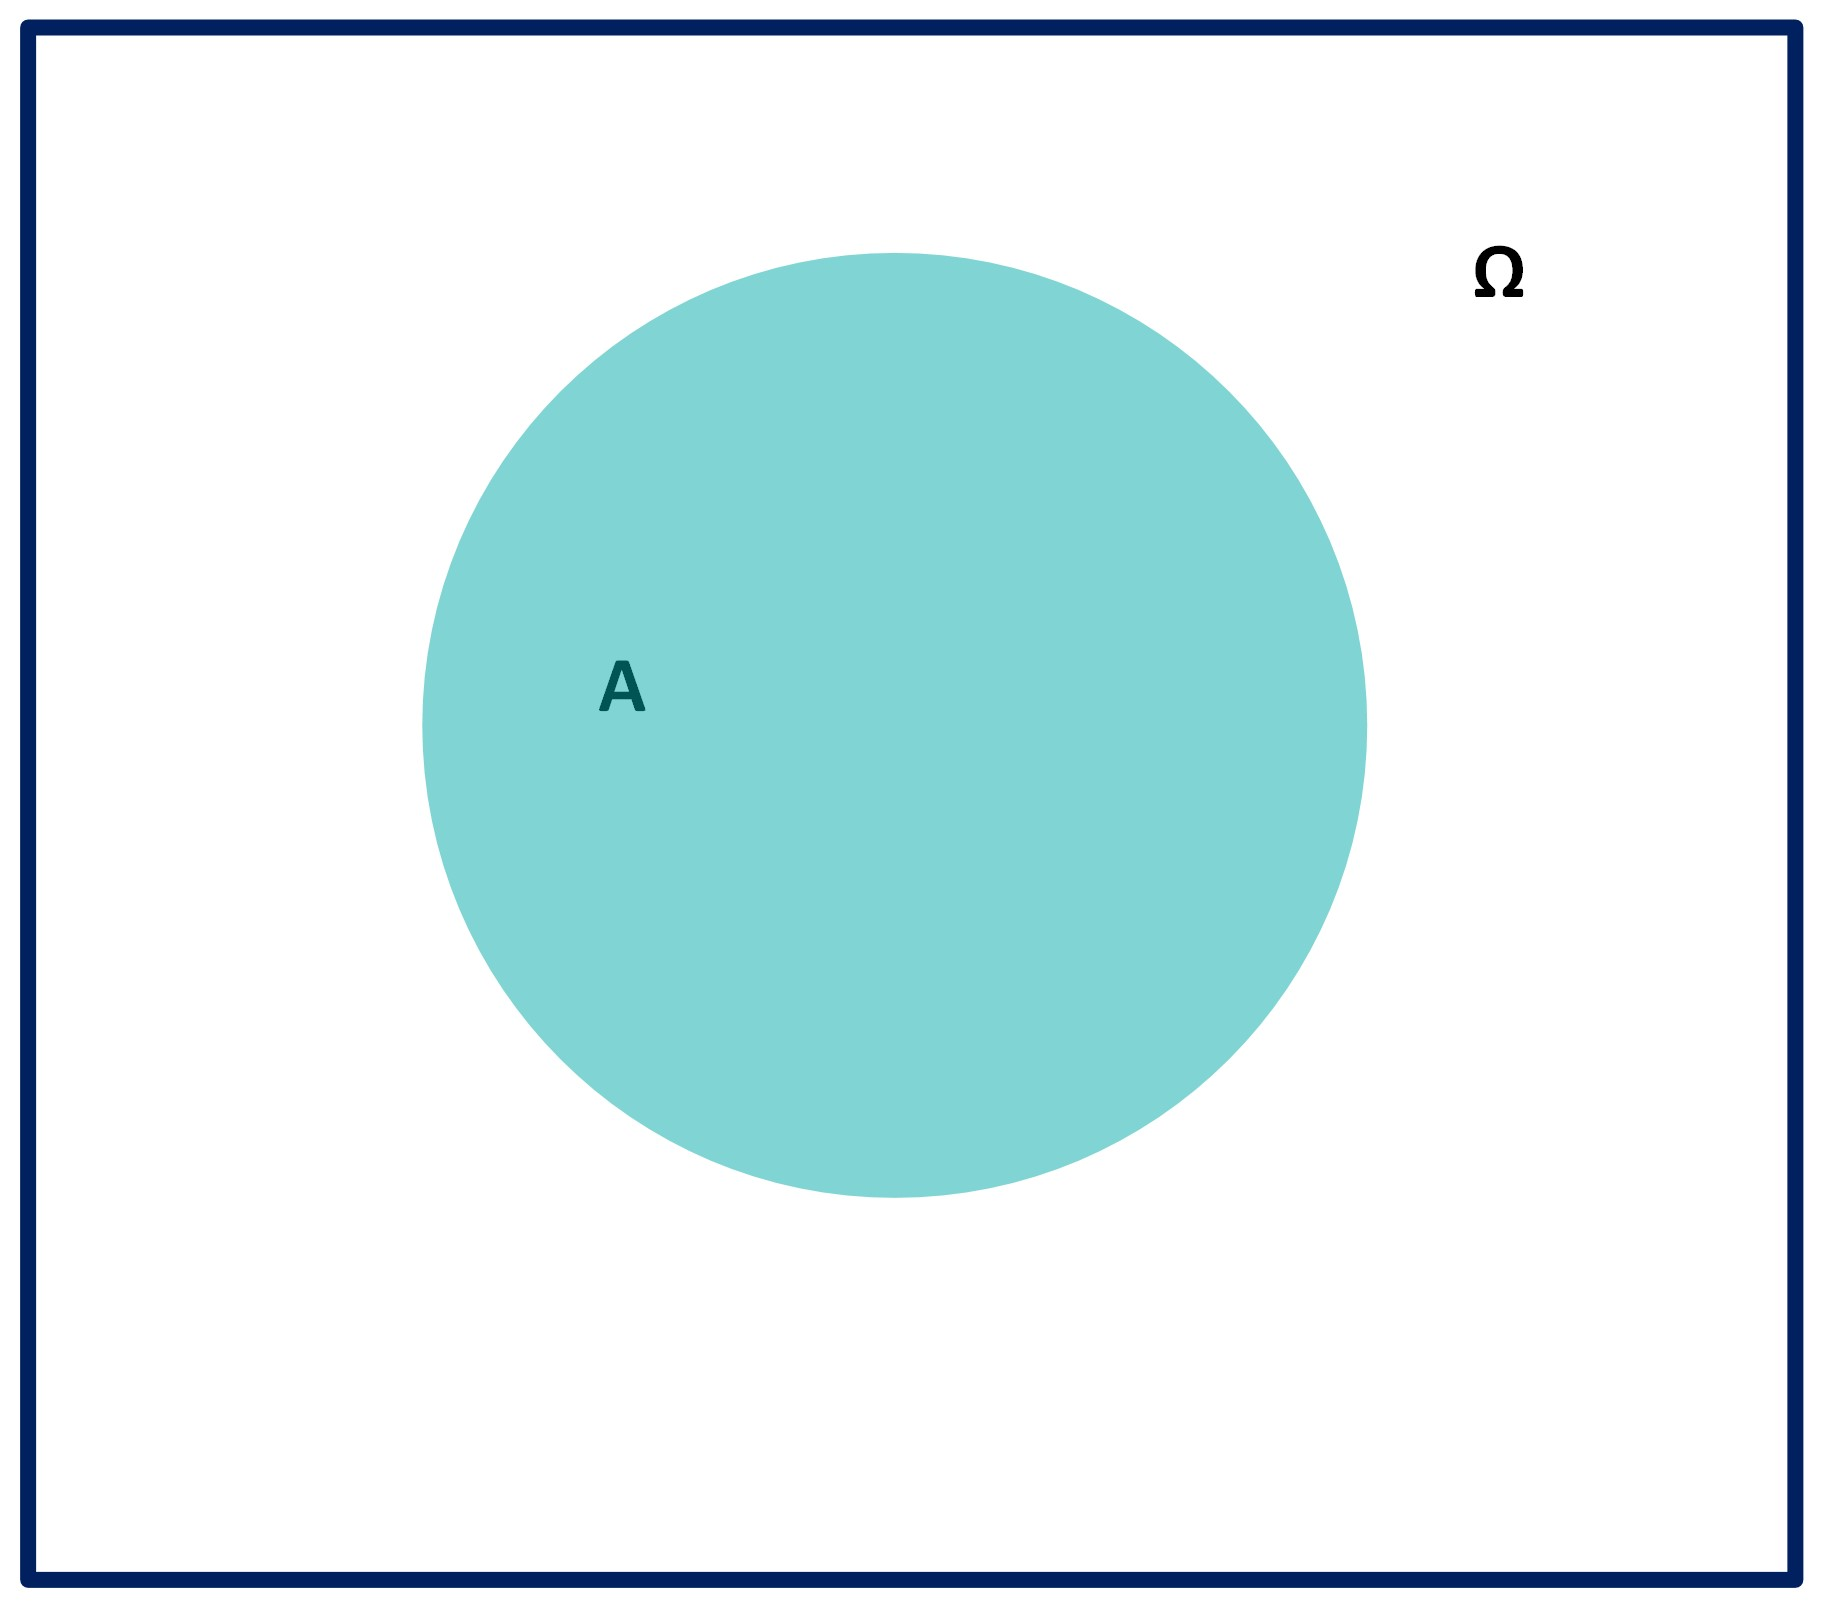
\includegraphics[width=\linewidth,height=1.5625in,keepaspectratio]{Images/venn1A_solo.jpeg} \\
\end{longtable}

Leyes de De Morgan

\[(A\cup B)^c=A^c\cap B^c\]

\begin{longtable}[]{@{}
  >{\centering\arraybackslash}p{(\linewidth - 2\tabcolsep) * \real{0.5000}}
  >{\centering\arraybackslash}p{(\linewidth - 2\tabcolsep) * \real{0.5000}}@{}}
\toprule\noalign{}
\begin{minipage}[b]{\linewidth}\centering
\(A\cup B\)
\end{minipage} & \begin{minipage}[b]{\linewidth}\centering
\((A\cup B)^c\)
\end{minipage} \\
\midrule\noalign{}
\endhead
\bottomrule\noalign{}
\endlastfoot
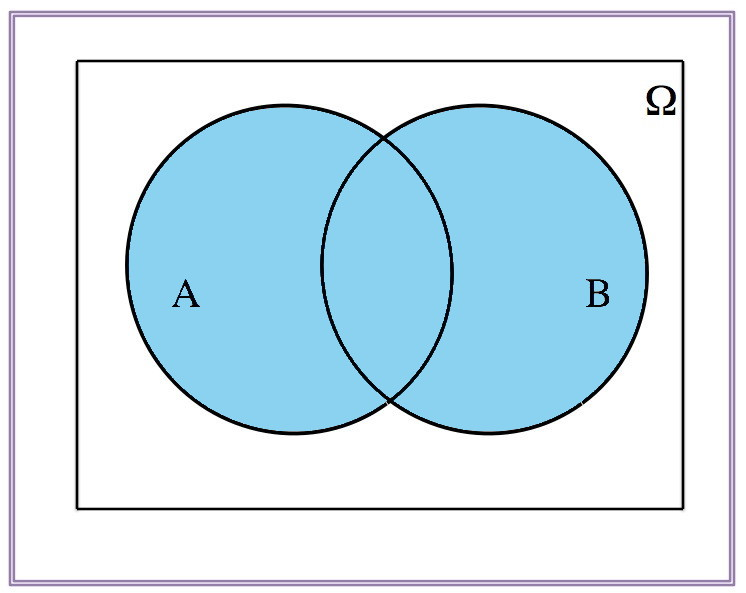
\includegraphics[width=\linewidth,height=1.5625in,keepaspectratio]{Images/proba1dibujos/demorgan6.jpg}
&
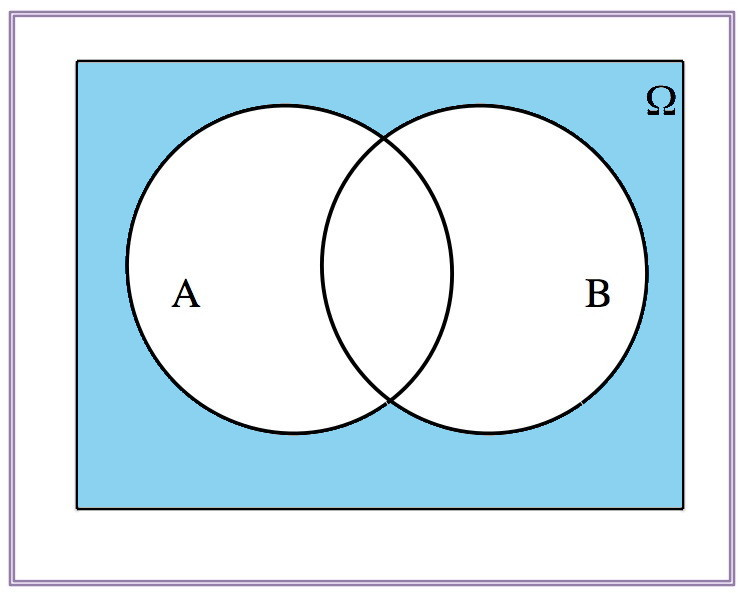
\includegraphics[width=\linewidth,height=1.5625in,keepaspectratio]{Images/proba1dibujos/demorgan7.jpg} \\
\end{longtable}

\[(A\cup B)^c=A^c\cap B^c\]

\begin{longtable}[]{@{}
  >{\centering\arraybackslash}p{(\linewidth - 4\tabcolsep) * \real{0.3333}}
  >{\centering\arraybackslash}p{(\linewidth - 4\tabcolsep) * \real{0.3333}}
  >{\centering\arraybackslash}p{(\linewidth - 4\tabcolsep) * \real{0.3333}}@{}}
\toprule\noalign{}
\begin{minipage}[b]{\linewidth}\centering
\(A^c\)
\end{minipage} & \begin{minipage}[b]{\linewidth}\centering
\(B^c\)
\end{minipage} & \begin{minipage}[b]{\linewidth}\centering
\(A^c\cap B^c\)
\end{minipage} \\
\midrule\noalign{}
\endhead
\bottomrule\noalign{}
\endlastfoot
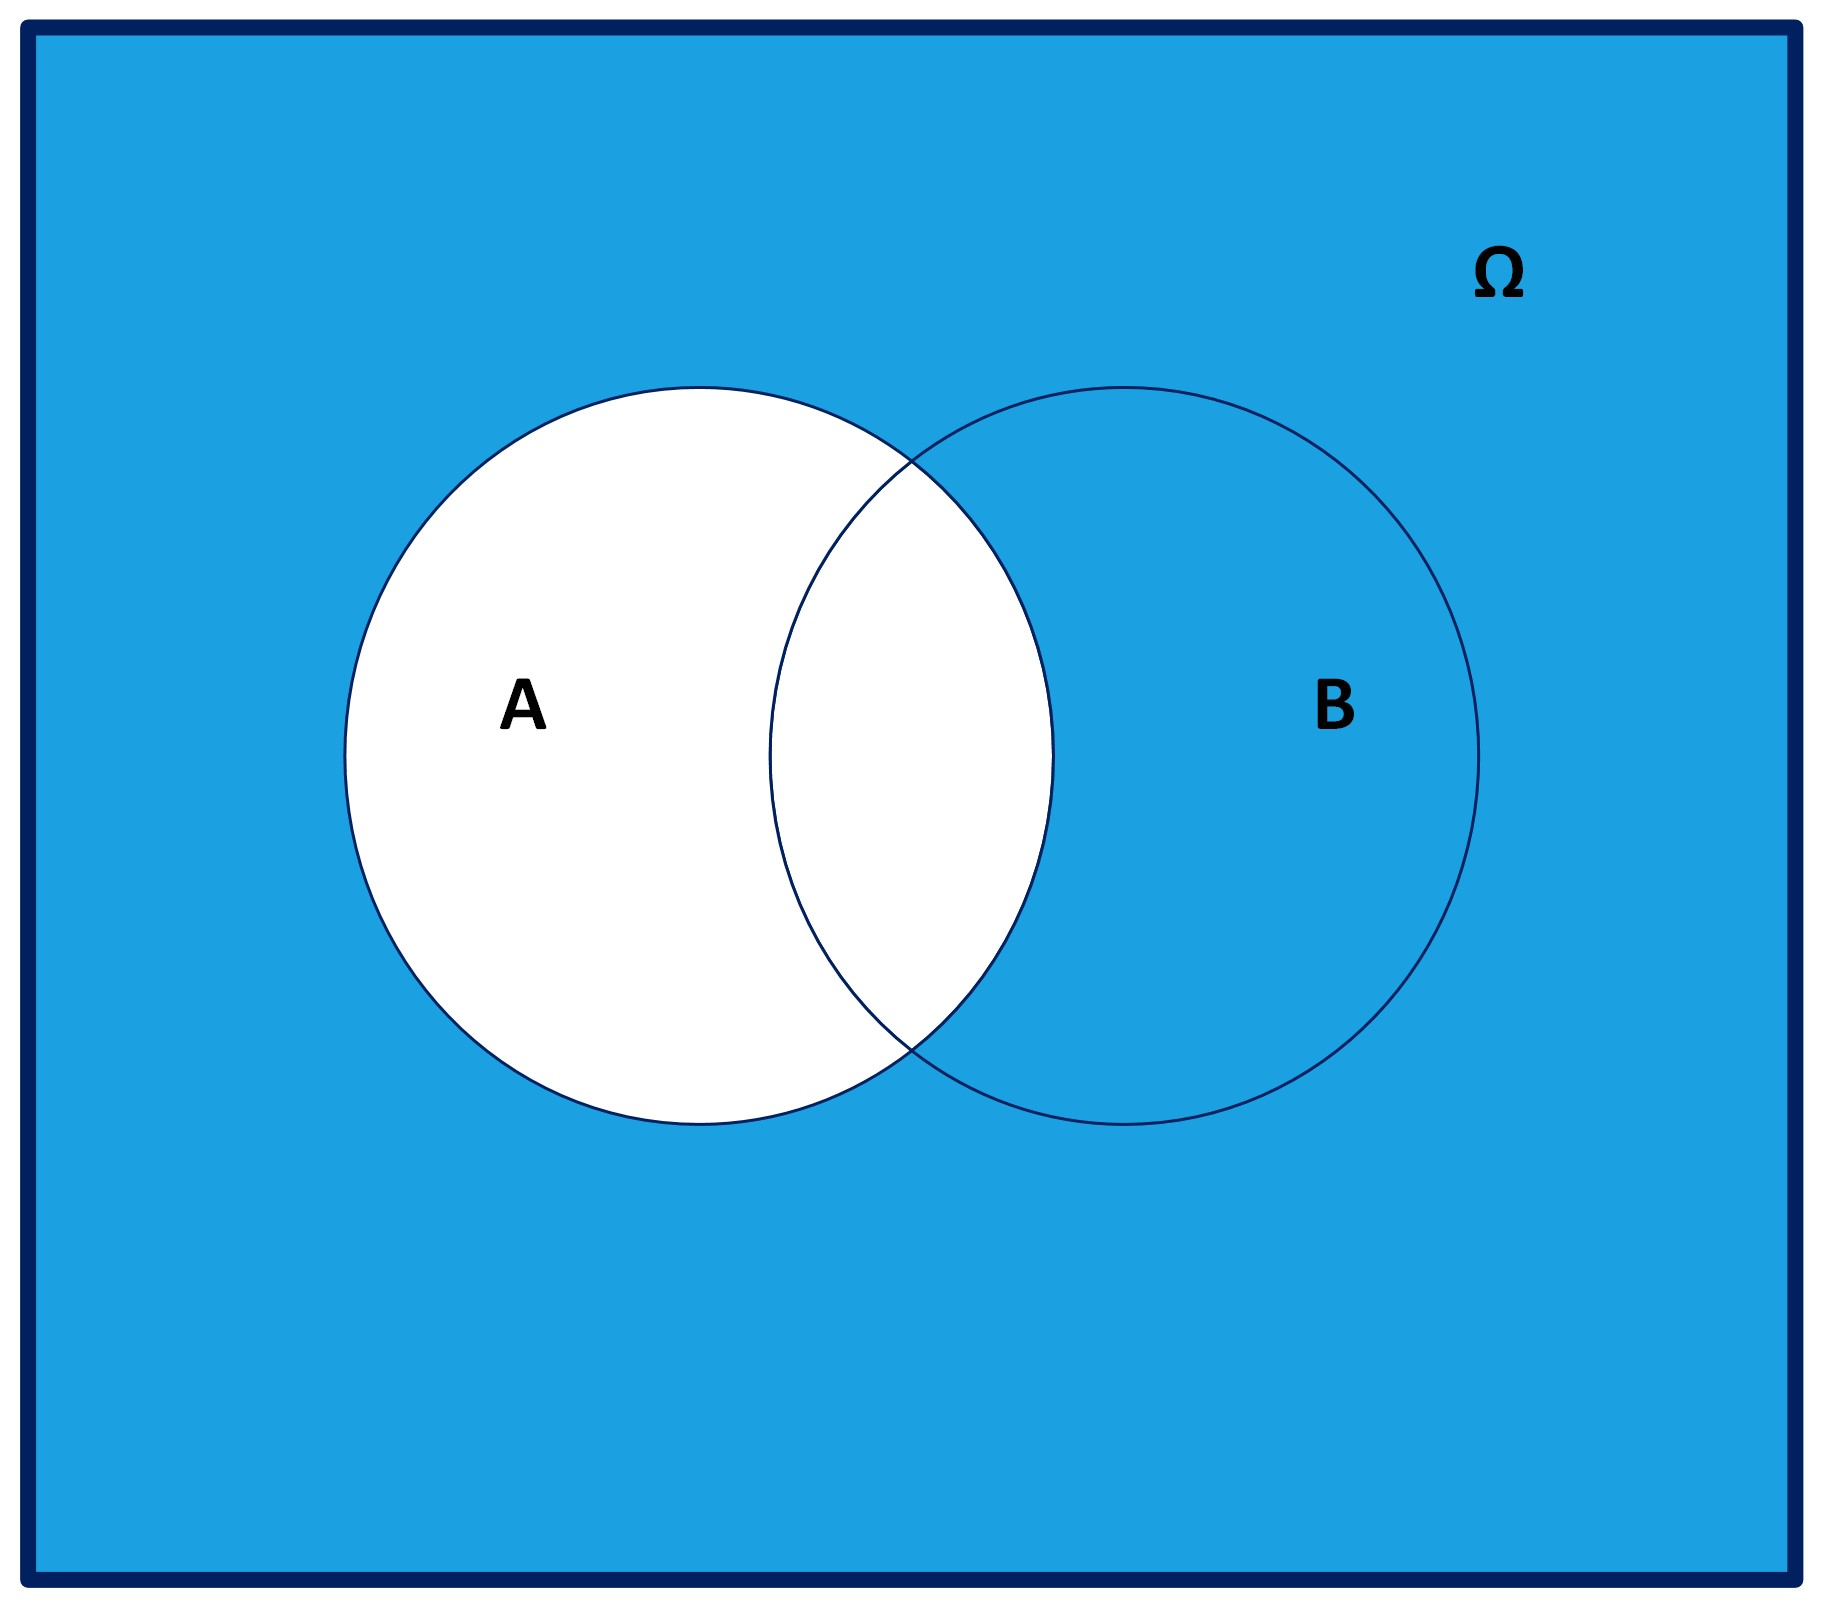
\includegraphics[width=\linewidth,height=1.5625in,keepaspectratio]{Images/venn1Ac_conB.jpeg}
&
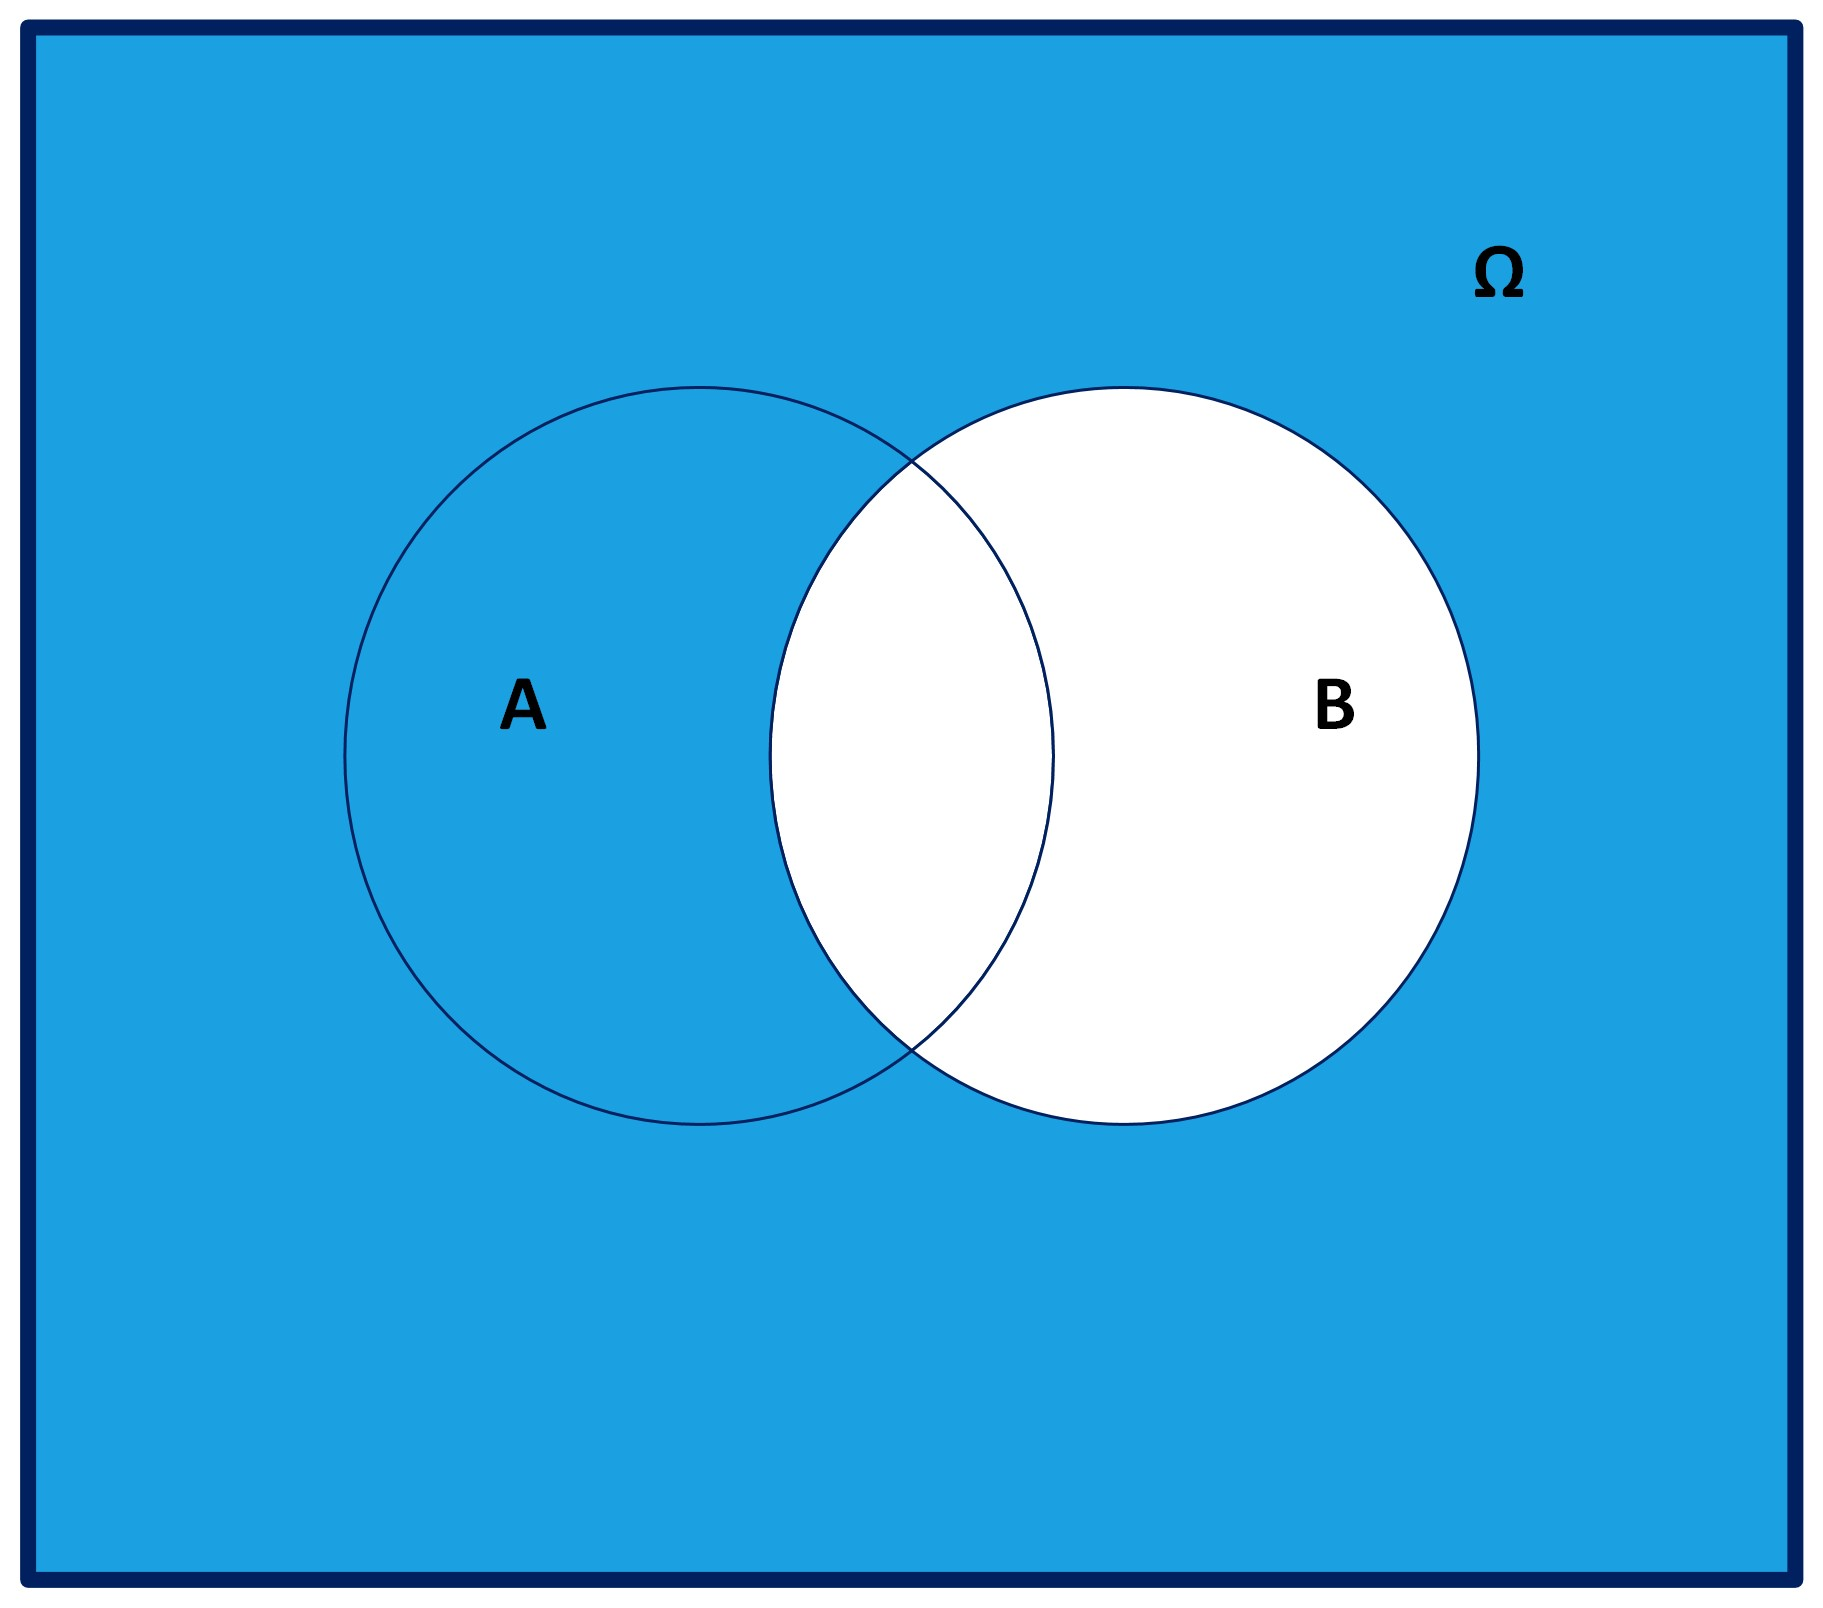
\includegraphics[width=\linewidth,height=1.5625in,keepaspectratio]{Images/venn1Bc_conA.jpeg}
&
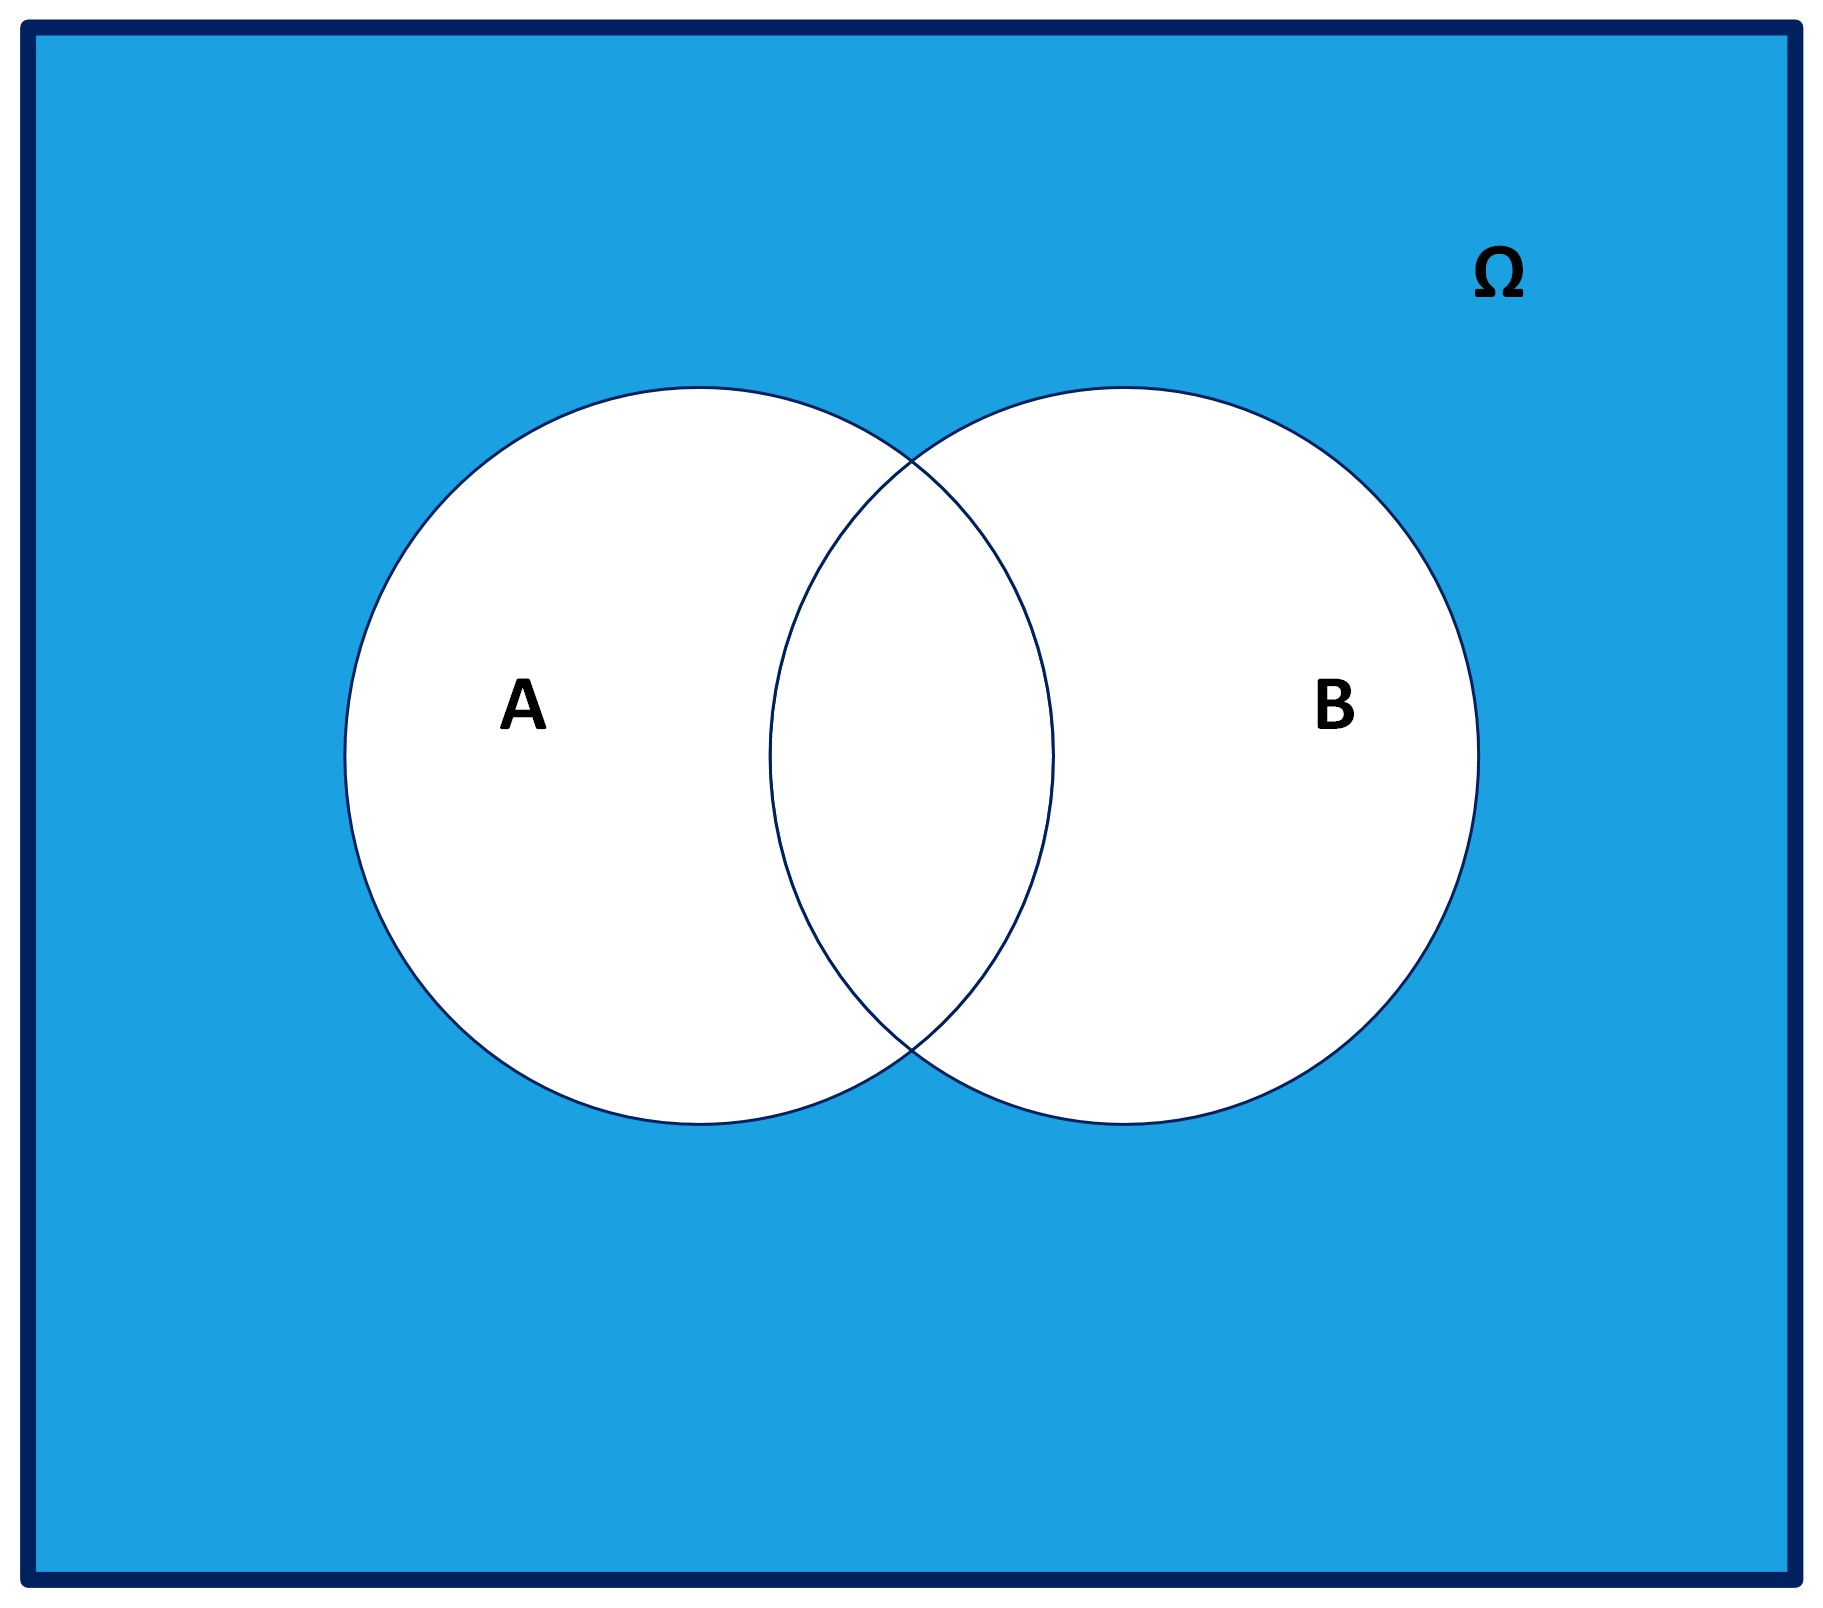
\includegraphics[width=\linewidth,height=1.5625in,keepaspectratio]{Images/venn1interseccioncomplementarios.jpeg} \\
\end{longtable}

\[(A\cap B)^c=A^c\cup B^c\]

\begin{longtable}[]{@{}
  >{\centering\arraybackslash}p{(\linewidth - 2\tabcolsep) * \real{0.5000}}
  >{\centering\arraybackslash}p{(\linewidth - 2\tabcolsep) * \real{0.5000}}@{}}
\toprule\noalign{}
\begin{minipage}[b]{\linewidth}\centering
\(A\cap B\)
\end{minipage} & \begin{minipage}[b]{\linewidth}\centering
\((A\cap B)^c\)
\end{minipage} \\
\midrule\noalign{}
\endhead
\bottomrule\noalign{}
\endlastfoot
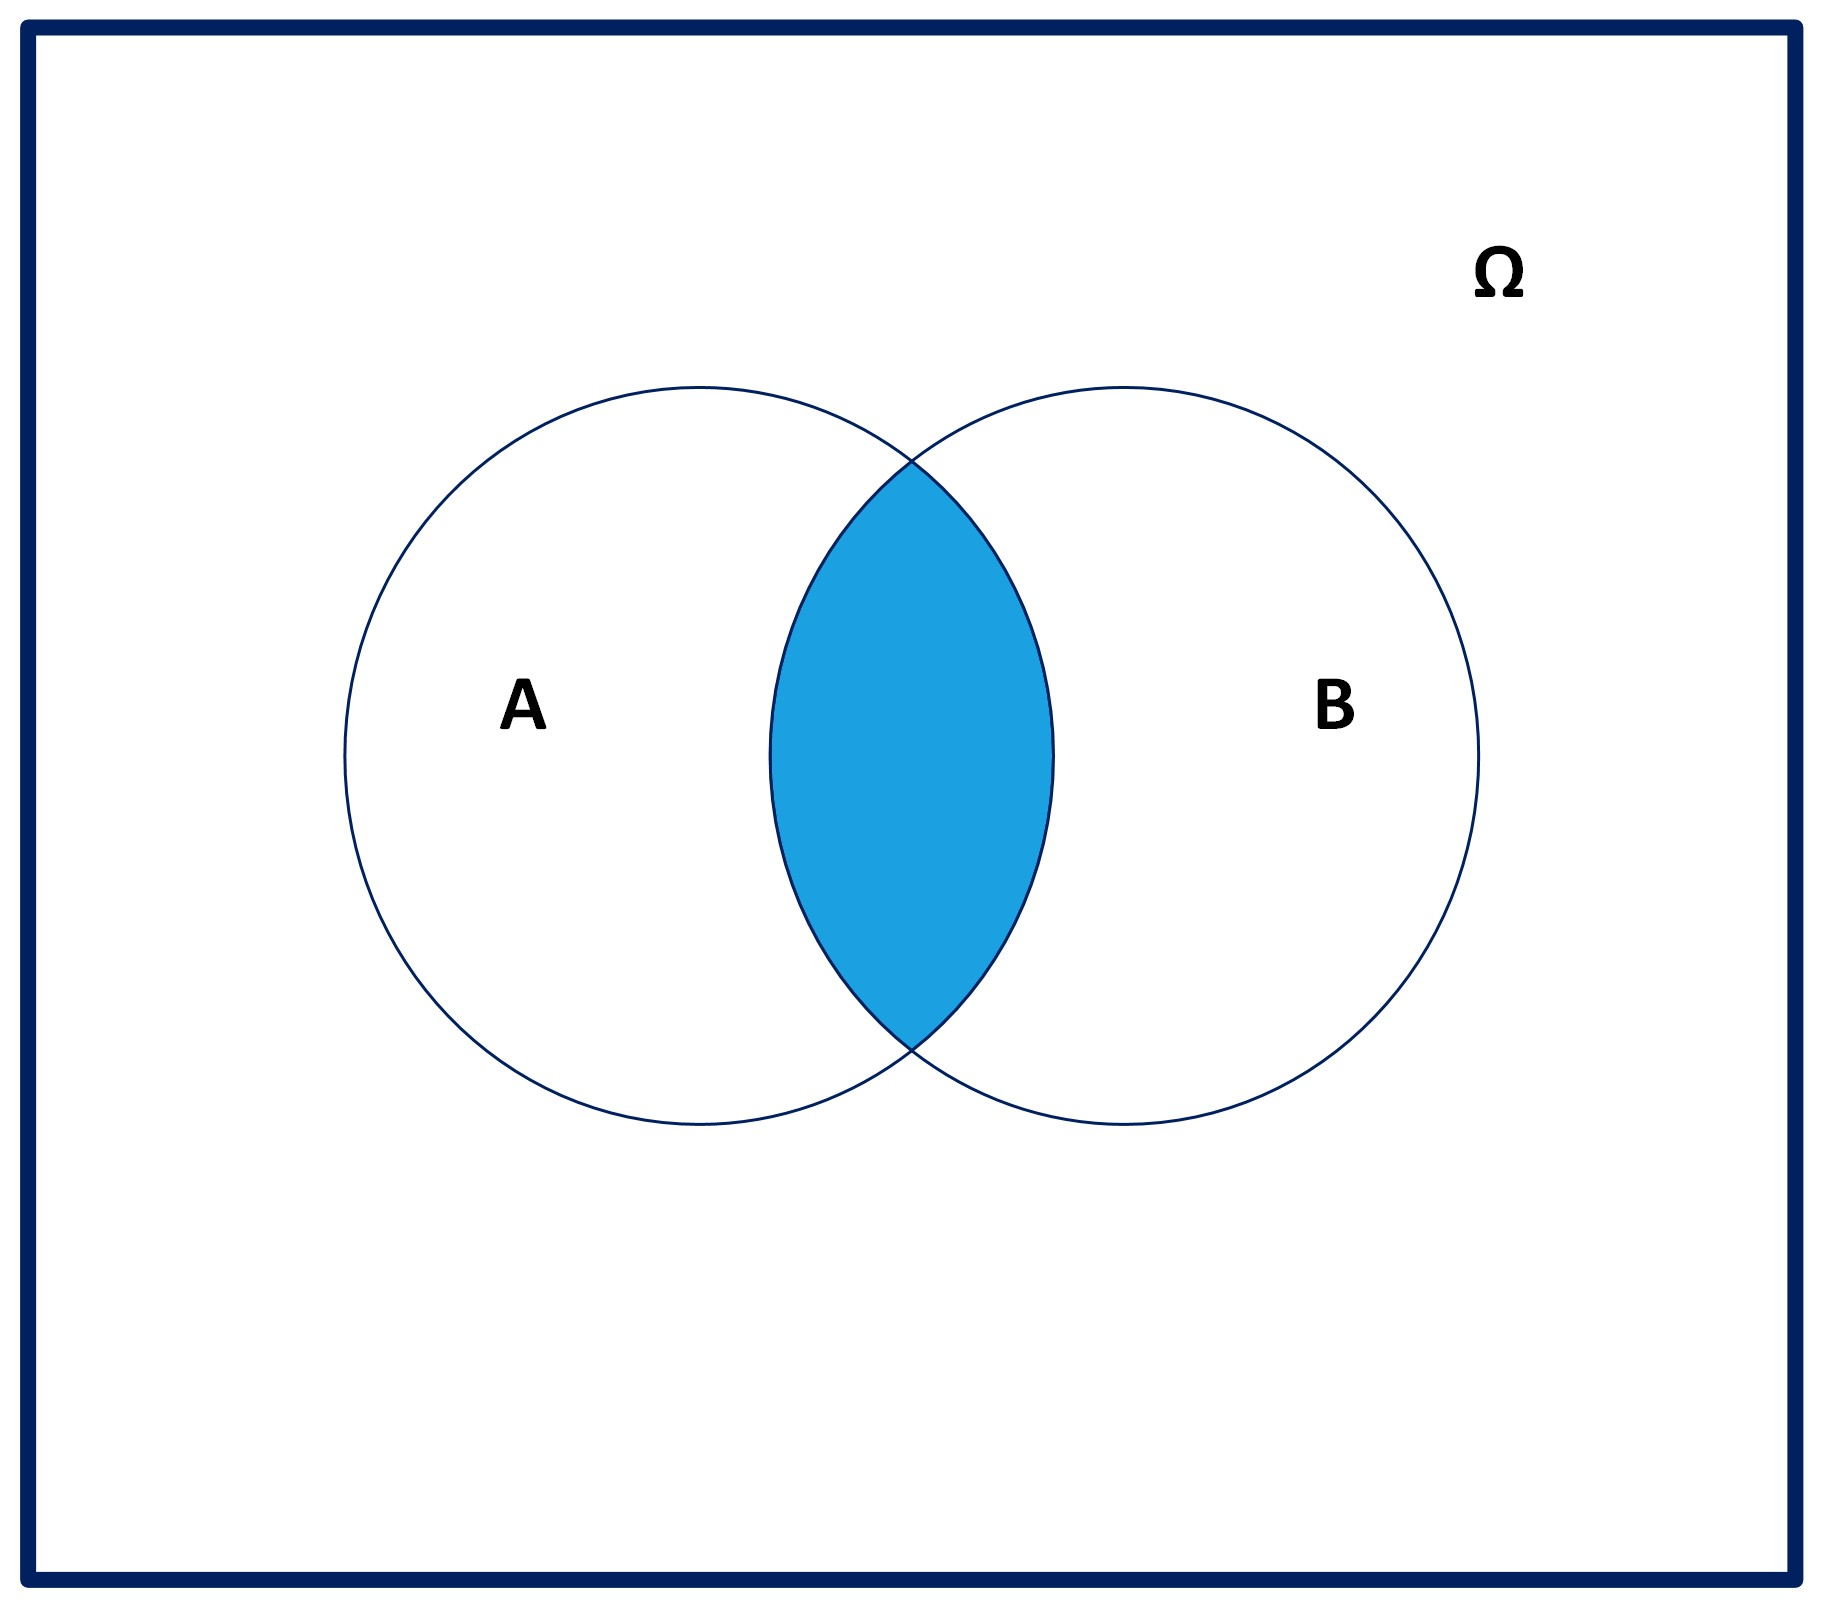
\includegraphics[width=\linewidth,height=1.5625in,keepaspectratio]{Images/venn1AyB.jpeg}
&
\includegraphics[width=\linewidth,height=1.51042in,keepaspectratio]{Images/venn1ComplementarioInterseccion.jpeg} \\
\end{longtable}

\[(A\cap B)^c=A^c\cup B^c\]

\begin{longtable}[]{@{}
  >{\centering\arraybackslash}p{(\linewidth - 4\tabcolsep) * \real{0.3333}}
  >{\centering\arraybackslash}p{(\linewidth - 4\tabcolsep) * \real{0.3333}}
  >{\centering\arraybackslash}p{(\linewidth - 4\tabcolsep) * \real{0.3333}}@{}}
\toprule\noalign{}
\begin{minipage}[b]{\linewidth}\centering
\(A^c\)
\end{minipage} & \begin{minipage}[b]{\linewidth}\centering
\(B^c\)
\end{minipage} & \begin{minipage}[b]{\linewidth}\centering
\(A^c\cup B^c\)
\end{minipage} \\
\midrule\noalign{}
\endhead
\bottomrule\noalign{}
\endlastfoot
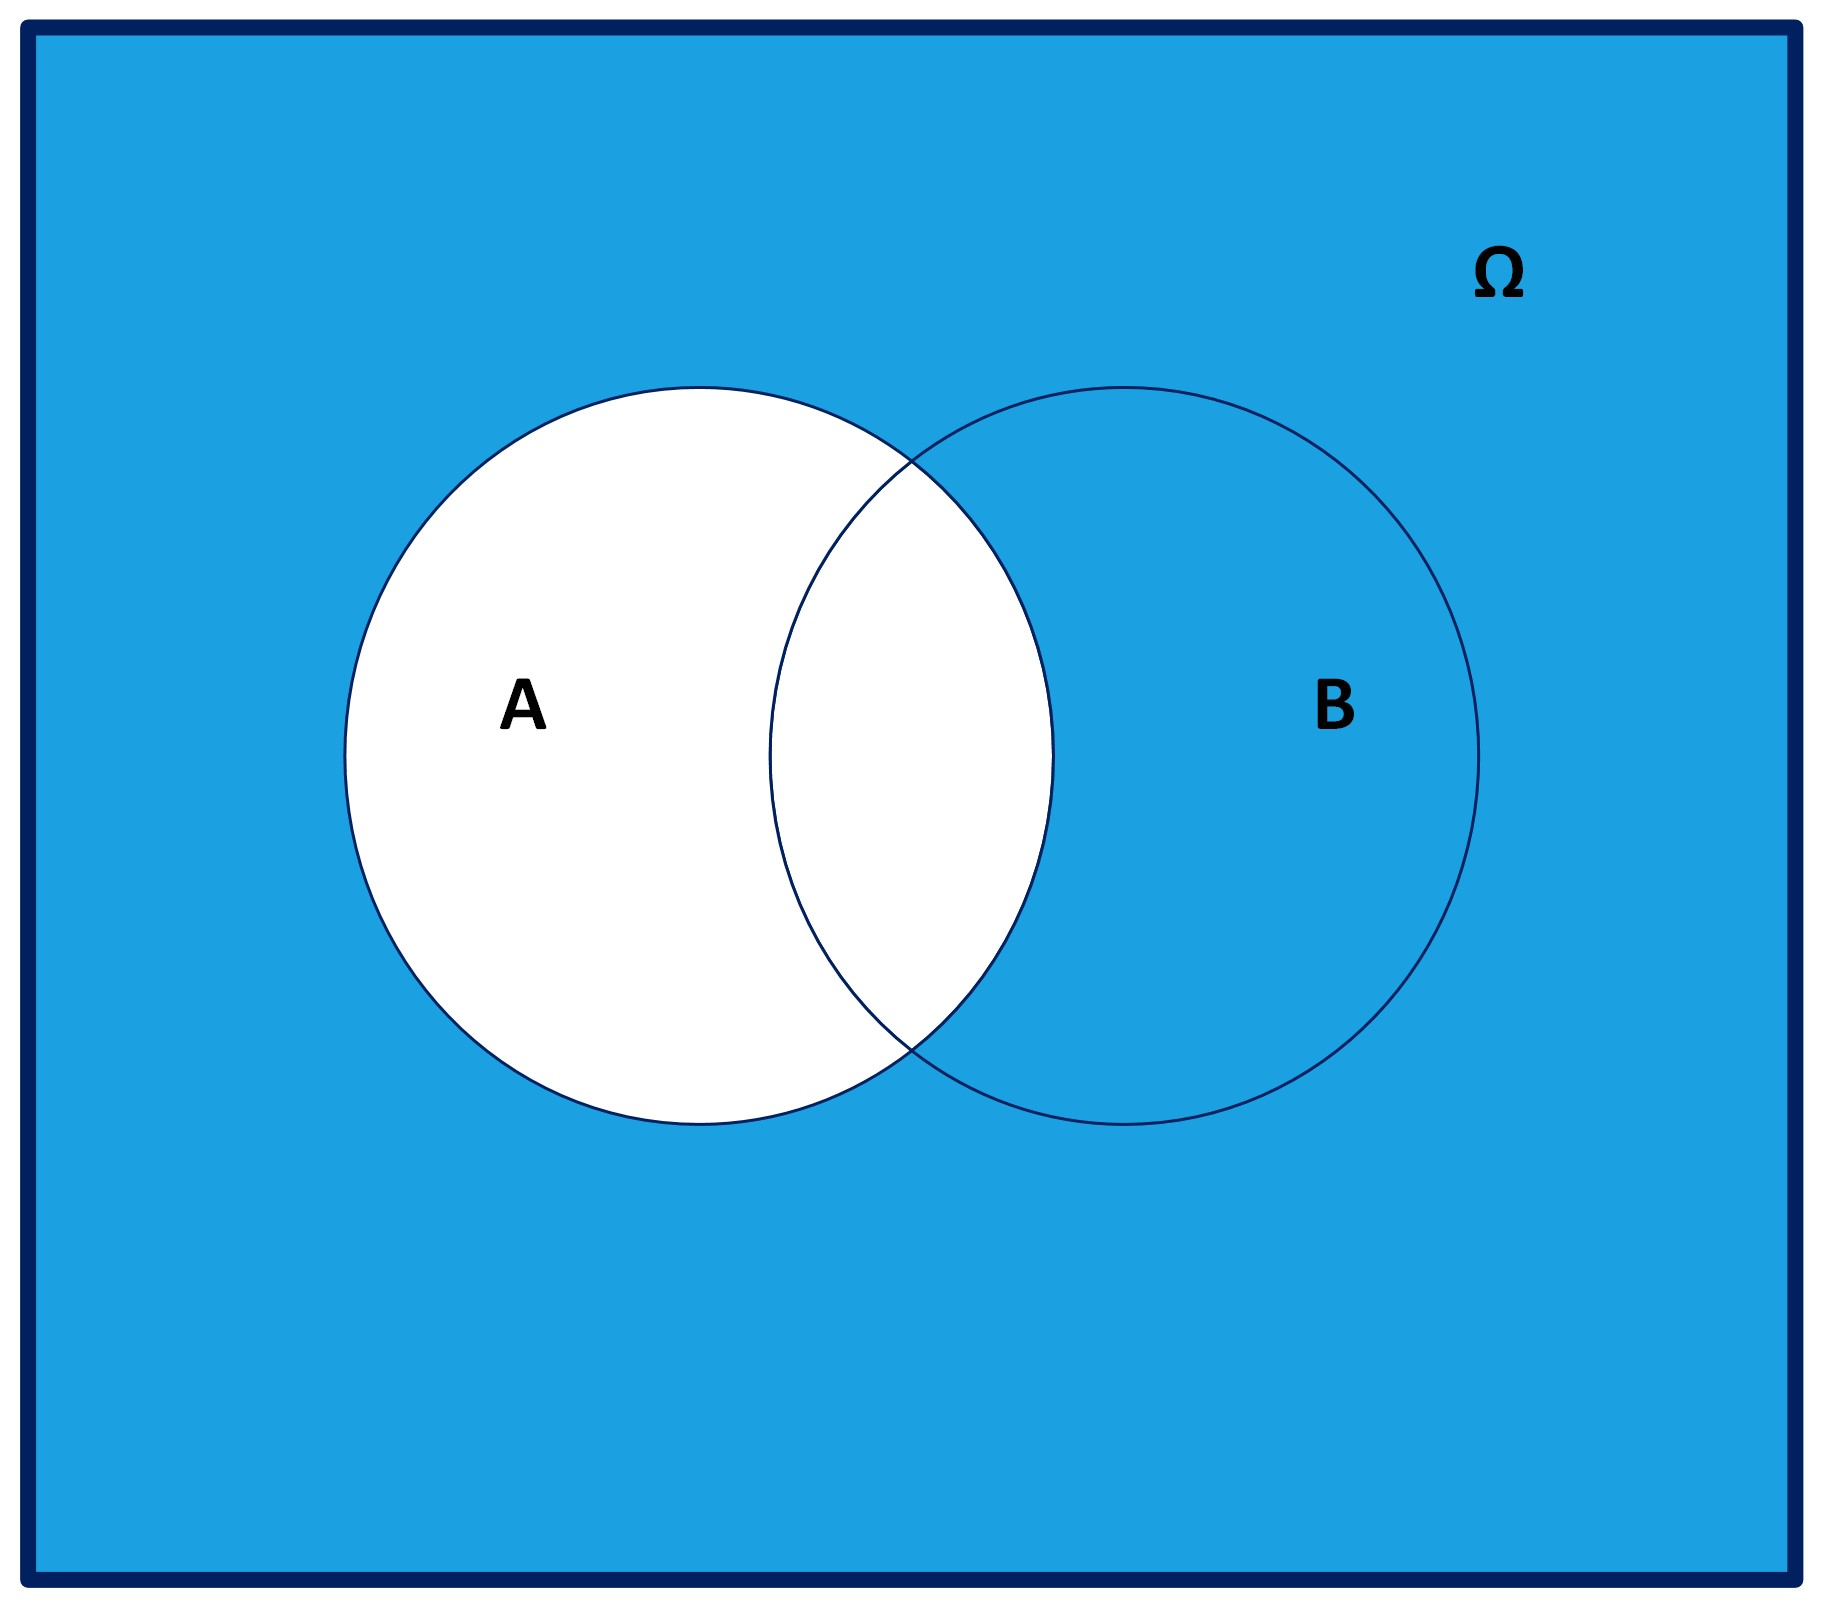
\includegraphics[width=\linewidth,height=1.5625in,keepaspectratio]{Images/venn1Ac_conB.jpeg}
&
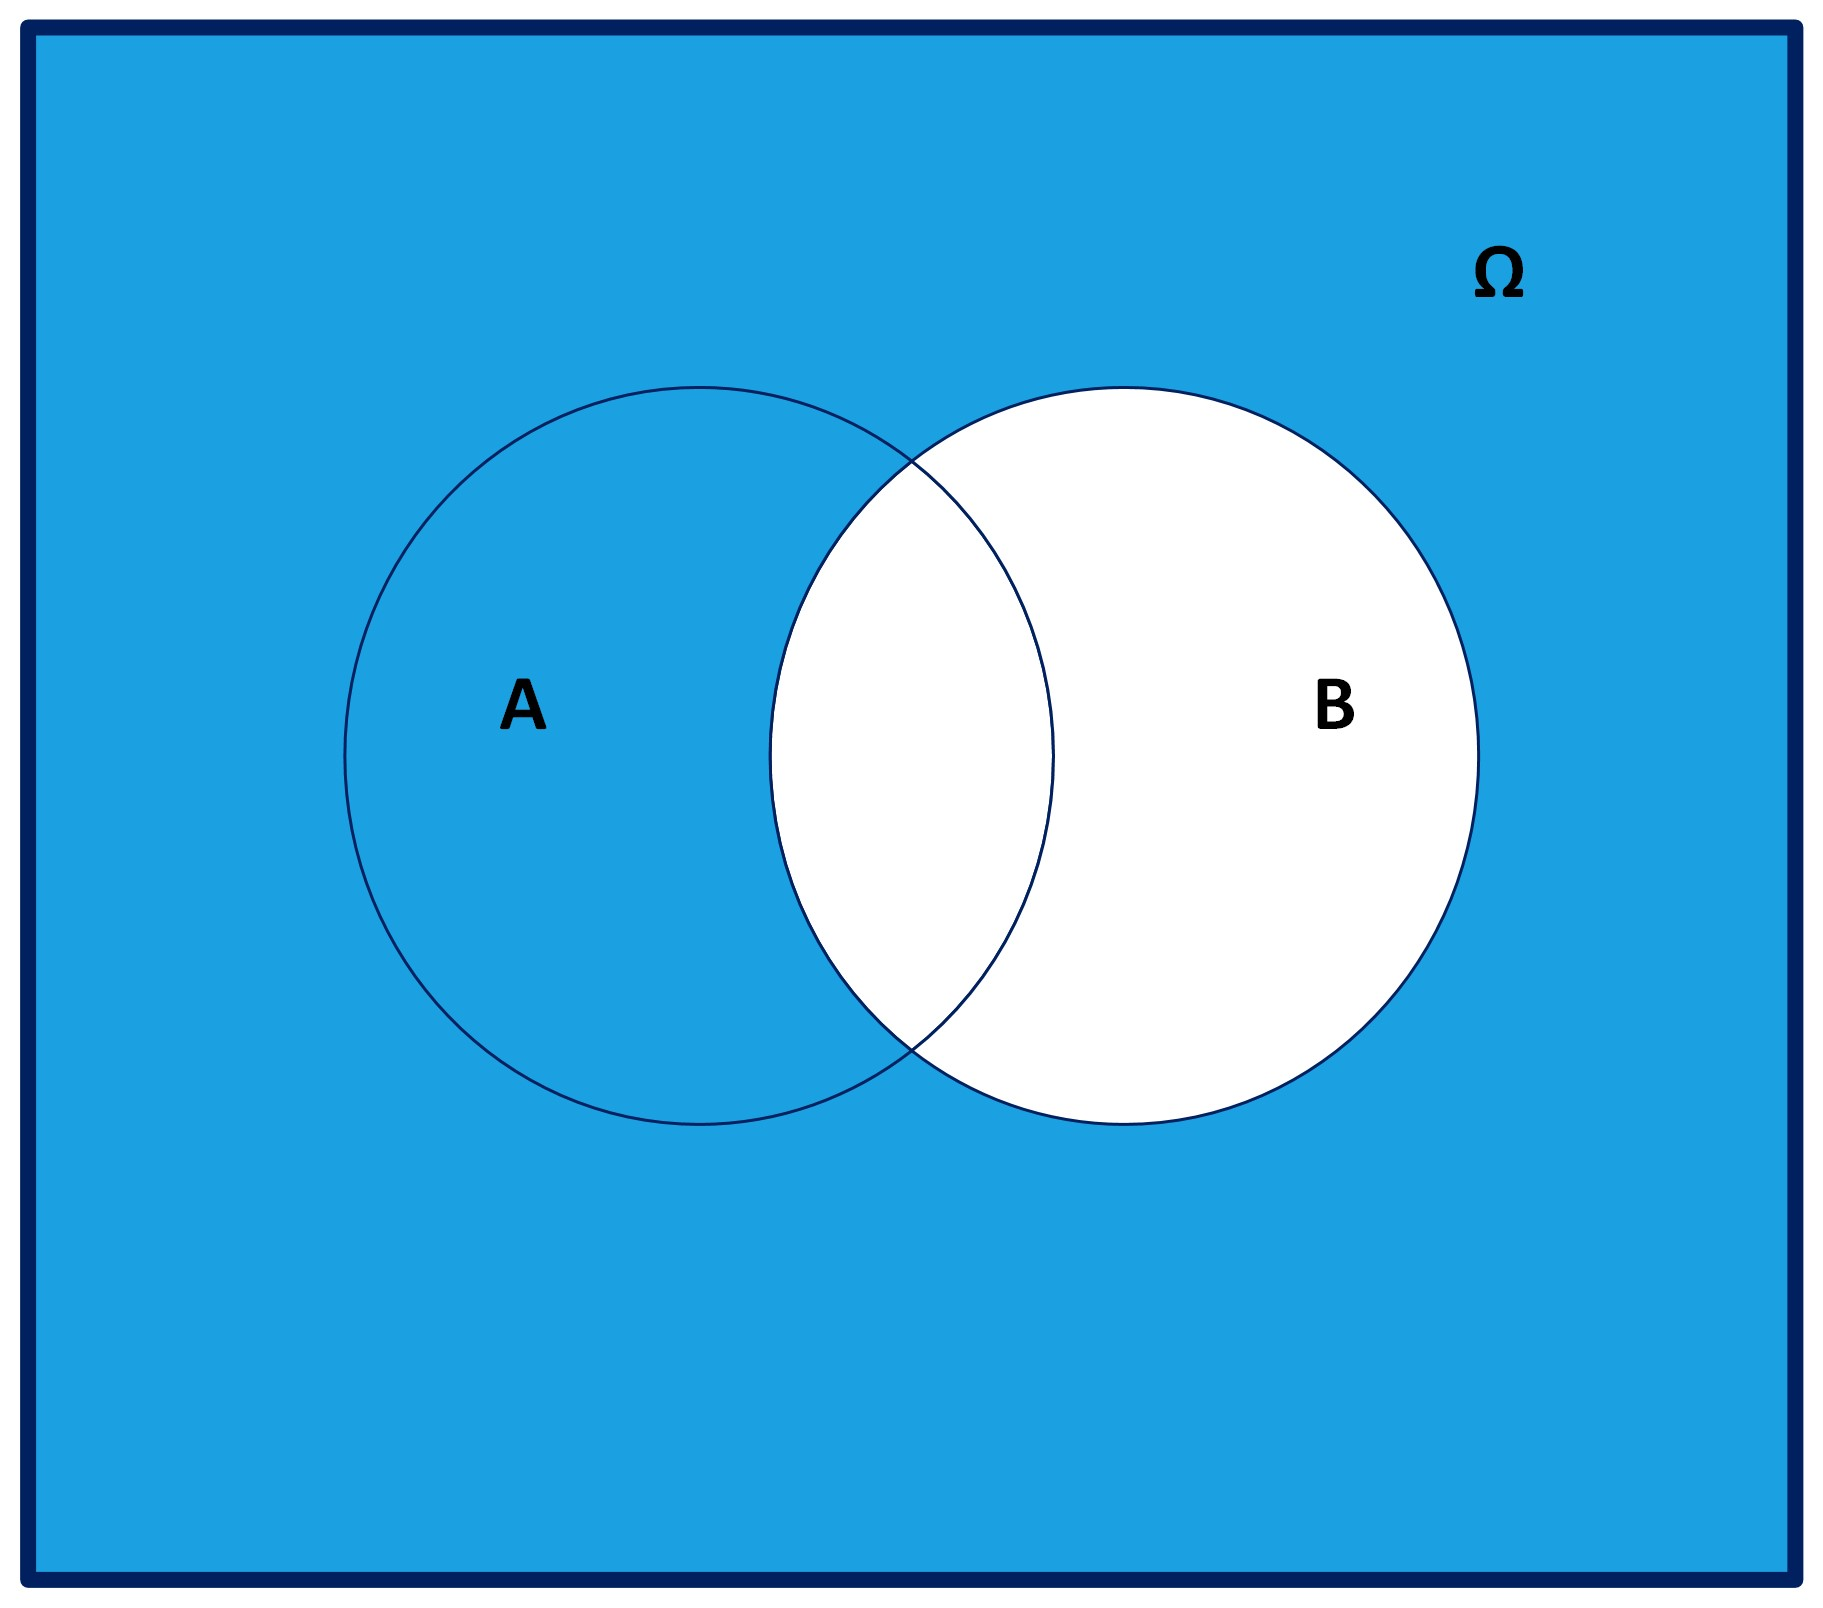
\includegraphics[width=\linewidth,height=1.5625in,keepaspectratio]{Images/venn1Bc_conA.jpeg}
&
\includegraphics[width=\linewidth,height=1.51042in,keepaspectratio]{Images/venn1ComplementarioInterseccion.jpeg} \\
\end{longtable}

\section{Definición de
probabilidad}\label{definiciuxf3n-de-probabilidad}

La probabilidad de un suceso es una puntuación (\emph{score}) numérico
entre 0 y 1 que mide la verosimilitud de que este evento se produzca.

Esta verosimilitud puede estar justificada por:

\begin{itemize}
\item
  Estimación personal
\item
  Estimación de expertos
\item
  La frecuencia con la que se da
\item
  Cálculo formal
\end{itemize}

Definición formal de probabilidad

Sea \(\Omega\) el espacio muestral de un experimento aleatorio.
Supongamos que el número de posibles resultados, por el momento, es
finito.

Una probabilidad sobre \(\Omega\) es una aplicación
\(P:\mathcal{P}(\Omega)\to [0,1]\) con las siguientes propiedades:

\begin{enumerate}
\def\labelenumi{\arabic{enumi}.}
\tightlist
\item
  \(0\leq P(A)\leq 1\), para todo suceso \(A\).
\item
  \(P(\Omega)=1\).
\item
  Si \(\{A_1,A_2,\ldots,A_n\}\) son sucesos disjuntos dos a dos,
  entonces
\end{enumerate}

\[
P(A_1\cup A_2\cup \cdots \cup A_n)=P(A_1)+P(A_2)+\cdots +P(A_n)
\]

Si \(a\in \Omega\) es un suceso elemental cometeremos el abuso de
notación de poner \(P(a)\) en lugar de \(P(\{a\})\).

Veamos un ejemplo real de cómo se calcula la probabilidad de un suceso.

Ejemplo

En la página de la
\href{http://www.donasang.org/que-es-la-sang/es_frequencies-dels-diferents-grups.html}{Fundación
Banco de Sangre y Tejidos de las Islas Baleares (17-08-2023)} podemos
encontrar información sobre los porcentajes de tipos de sangre de los
donantes de las Islas Baleares:

\[A: 46\%;\  B: 7.5\%;\  AB: 3.5\%;\  O: 43\%.\]

¿Cuál es la probabilidad de que un balear donante de sangre no sea del
tipo O?

\textbf{Experimento aleatorio:} tipo de sangre de un paciente humano:

\[\Omega=\{\mbox{A,B,AB,O}\}\]

\textbf{Probabilidad} de un suceso: se asimila al porcentaje observado
de individuos.

\textbf{Suceso:} \(\{\mbox{O}\}^c=\{\mbox{A,B,AB}\}\).

\[P(\{\mbox{O}\}^c)\!=\!P(\{\mbox{A,B,AB}\})\!=\!
P(\mbox{A})+P (\mbox{B})+P(\mbox{AB})\!=\!0.57.\]

Necesitaremos tener propiedades y fórmulas prácticas para poder calcular
probabilidades de sucesos más complejos. Veamos algunas de ellas.

Propiedades básicas de la probabilidad

\begin{itemize}
\item
  \(P(\emptyset)=0\).
\item
  \(\scriptsize{P(A-B)=P(A)-P(A\cap B)}\) porque
  \(\scriptsize{P(A)=P(A-B)+P(A\cap B)}\).
\end{itemize}

\begin{center}
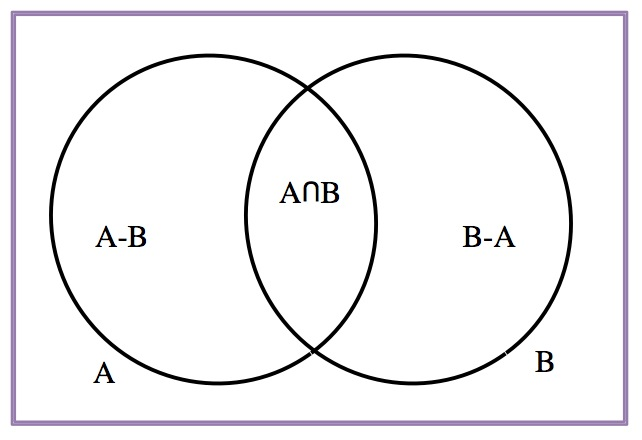
\includegraphics[width=0.3\linewidth,height=\textheight,keepaspectratio]{Images/proba1dibujos/A-B.jpg}
\end{center}

\begin{itemize}
\item
  Si \(B\subseteq A\), entonces \(0\leq P(B)\leq P(A)\).
\item
  \(P(A^c)=1-P(A)\).
\end{itemize}

Una identidad muy utilizada es la de la probabilidad de la unión de dos
sucesos cualesquiera.

La Probabilidad de la unión de dos sucesos

\(P(A\cup B)=P(A)+P(B)-P(A\cap B)\)

\begin{center}
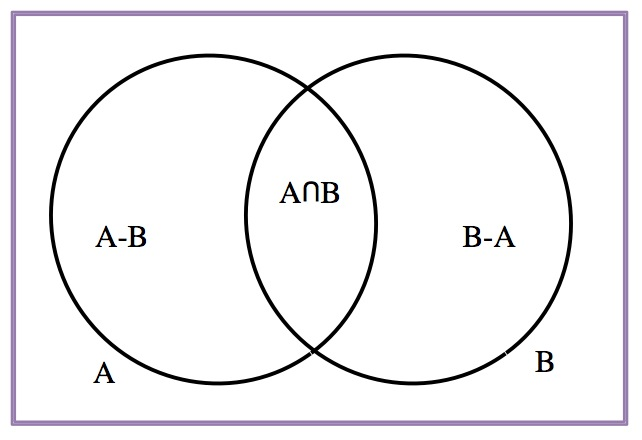
\includegraphics[width=0.6\linewidth,height=\textheight,keepaspectratio]{Images/proba1dibujos/A-B.jpg}
\end{center}

La demostración analítica de esta propiedad es la siguiente:

\begin{eqnarray*}
P(A)+P(B)-P(A\cap B) &=& P(A-B)+P(A\cap B)\\ 
& & +P(B-A)+ P(A\cap  B)-P(A\cap  B)\\
&=& P(A-B)+P(A\cap B)+ P(B-A) \\
&=& P(A\cup B).\\
\end{eqnarray*}

Probabilidad de la unión de \(n\) conjuntos

Sean \(A_1, A_2,\ldots A_n\) sucesos. Entonces:

\[
P(\cup_{i=1}^n A_i)=\sum_{i=1}^n P(A_i)-\sum_{1\leq i<j\leq n}P(A_i\cap A_j)+\cdots +(-1)^{n-1}P(A_1\cap A_2\cap \cdots \cap A_n).
\]

La demostración es sncilla por inducción, ya tenemos el caso de dos
sucesos, suponemos que es cierta para \(n\) y la extendemos a \(n+1\)
sucesos.

A modo de comprobación veamos un ejemplo genérico con tres sucesos

\(A=\{1,4,5,6\}\), \(B=\{2,4,6,7\}\) y \(C=\{3,5,6,7\}\). En este caso
la fórmula nos da

\[
P(A\cup B\cup C)= & P(A)+P(B)+P(C)-P(A\cap B)-P(A\cap C)
-P(B\cap C)+P(A\cap B\cap C).
\]

Gráficamente tenemos esta situación:

\begin{center}
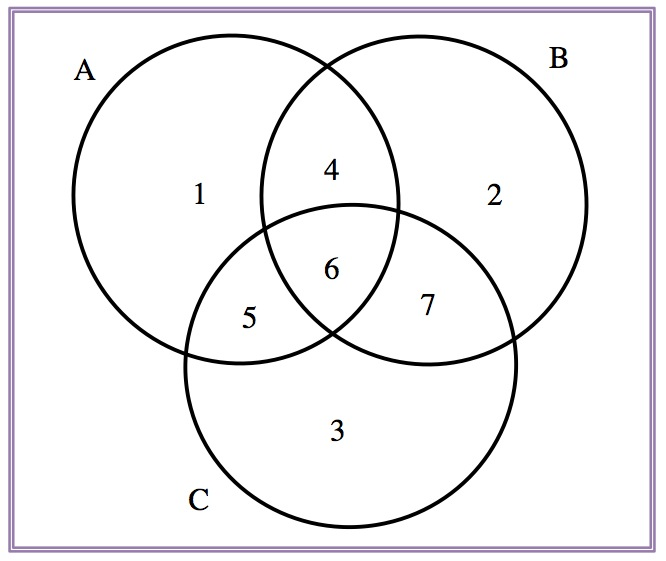
\includegraphics[width=0.3\linewidth,height=\textheight,keepaspectratio]{Images/proba1dibujos/tresconjunts.jpg}
\end{center}

Ahora podemos comprobar la fórmula para este caso.

\begin{eqnarray*}
P(A\cup B\cup C)&=&P(A)+P(B)+P(C)-P(A\cap B) \\
  & & - P(A\cap C)-P(B\cap C)+P(A\cap B\cap C).\\
\end{eqnarray*}

Efectivamente tenemos que:

\[P(A\cup B\cup C)=P(1)+P(2)+P(3)+P(4)+P(5)+P(6)+P(7).\]

Una de las formas más intuitiva de asignación de probabilidades es hacer
el cociente entre los casos favorables a que acontezca el vento y los
casos posibles del experimento; la llmadad fórmula de Laplace.

Propiedad

\begin{itemize}
\item
  En general dado un suceso \(A=\{a_1,a_2,\ldots,a_k\}\), entonces \[
  P(A)=P(a_1)+P(a_2)+\cdots+P(a_k).
  \]
\item
  \textbf{Fórmula de Laplace}: Si todos los sucesos elementales tienen
  la misma probabilidad, \[
  P(A)=\frac{|A|}{|\Omega|}\Big(=\frac{\mbox{casos favorables}}{\mbox{casos posibles}}\Big).
  \]
\end{itemize}

En el procesamiento del lenguaje se suelen estudiar las frecucias de
plabaras o letras de un determinado idioma. Veamos un ejemplo sobre las
frecuencias de las vocales en castellano.

Ejemplo: Frecuencia de vocales

Los porcentajes de vocales de un determinado idioma (de alfabeto latino)
según la
\href{https://es.wikipedia.org/wiki/Frecuencia_de_aparici\%C3\%B3n_de_letras}{Wikipedia}
son:

\[A: 18.7\%;\ E: 26.1\%;\ I: 25.7\%;\ O: 24.4\%;\ U: 5.1\%.\]

¿Cuál es la probabilidad que una vocal escogida al azar de este idioma
sea una E o una O?

El espacio muestral del experimento es \(\Omega=\{A,E,I,O,U\}\).

El suceso que deseamos analizar es \(\{E,0\}\).

Y su probabilidad es

\[P(\{E,O\})=P(E)+P(O)=0.261+0.244=0.505.\]

Otro ejemplo en este caso es sobre un test de drogas en el que se
analiza la presencia de cocaína y cannabis en la sangre de los
conductores, inspirado en un caso real.

Ejemplo: Consumo de drogas

Segun un árticulo de
\href{https://elpais.com/politica/2019/01/02/actualidad/1546426491_623324.html}{El
País}, en un control especial de la policía el \(0.1\%\) de todos los
conductores analizados en un control de tráfico dan positivo en un el
test en cocaína, y el \(1\%\) da positivo en cannabis. Un \(1.05\%\) da
positivo en alguno de los dos test.

¿Cuál es la probabilidad que un individuo analizado en el control de
drogas escogido al azar no de positivo en ninguno de lo dos test?

Los sucesos elementales del enunciado del problema son:

\begin{itemize}
\tightlist
\item
  \(A\): dar positivo en cocaína; \(P(A)=0.001.\)
\item
  \(B\): dar positivo en cannabis; \(P(B)=0.01.\)
\end{itemize}

En este caso nos interesa estudiar los sucesos:

\begin{itemize}
\tightlist
\item
  \(A\cup B\): dar positivo en alguno de los dos test;
  \(P(A\cup B)=0.0105.\)
\item
  \((A\cup B)^c\): no dar positivo en ninguno de los test,por tanto:
\end{itemize}

\[P((A\cup B)^c)=1-P(A\cup B)=1-0.0105=0.9895.\]

En un control especial de la policía el \(0.1\%\) de todos los
conductores analizados en un control de tráfico dan positivo en un el
test en cocaína, y el \(1\%\) da positivo en cannabis. Un \(1.05\%\) da
positivo en alguno de los dos test.

¿Cuál es la probabilidad que un analizado al azar de positivo en los dos
test en cocaína y cannabis?

Los sucesos elementales son:

\begin{itemize}
\tightlist
\item
  \(A\): dar positivo en cocaína; \(P(A)=0.001.\)
\item
  \(B\): dar positivo en cannabis; \(P(B)=0.01.\)
\end{itemize}

En este caso nos interesa estudiar los sucesos:

\begin{itemize}
\tightlist
\item
  \(A\cup B\): dar positivo en algún de los dos test;
  \(P(A\cup B)=0.0105.\)
\item
  \(A\cap B\): dar positivo en los dos test
\end{itemize}

de donde, por tanto:

\[\begin{array}{rl}
{P(A\cap B)} &{=P(A)+P(B)-P(A\cup B)}\\ &{=0.001+0.01-0.0105=0.0005}.
\end{array}\]

En un control especial de la policía el \(0.1\%\) de todos los
conductores analizados en un control de tráfico dan positivo en un el
test en cocaína, y el \(1\%\) da positivo en cannabis. Un \(1.05\%\) da
positivo en alguno de los dos test.

¿Cuál es la probabilidad de que un conductor analizado de positivo en
cocaína pero no en cannabis?

Los sucesos elementales son:

\begin{itemize}
\tightlist
\item
  \(A\): dar positivo en cocaína; \(P(A)=0.001.\)
\item
  \(B\): dar positivo en cannabis; \(P(B)=0.01.\)
\end{itemize}

En este caso nos interesa estudiar los sucesos:

\begin{itemize}
\tightlist
\item
  \(A\cap B\): dar positivo en los dos test; \(P(A\cap B)=0.0005.\)
\item
  \(A-B\): dar positivo en cocaína pero no en cannabis, por lo tanto
  tenemos que :
\end{itemize}

\[P(A-B) =P(A)-P(A\cap B) =0.001-0.0005=0.0005.\]

\section{Probabilidad condicionada}\label{probabilidad-condicionada}

Probabilidad condicionada

Dados dos sucesos \(A\) y \(B\), con \(P(A)>0\), la probabilidad
\(P(B|A)\) de \(B\) condicionado a \(A\) es la probabilidad

\begin{itemize}
\tightlist
\item
  de que suceda \(B\) suponiendo que pasa \(A\),
\item
  de que si pasa \(A\), entonces suceda \(B\),
\item
  de que un resultado de \(A\) también pertenezca a \(B\).
\end{itemize}

Se calcula a través de la definición:

\[
P(B|A)=\frac{P(A\cap B)}{P(A)}.
\]

Ejemplo

En una clase de 20 hombres y 30 mujeres, 15 hombres y 18 mujeres llevan
gafas. Contestemos las siguientes preguntas:

-sol - ¿Cuál es la probabilidad de que un alumno lleve gafas?

\[
\frac{33}{50}
\]

¿Cuál es la probabilidad de que un alumno sea mujer y lleve gafas?

\[
\frac{18}{50}
\]

¿Cuál es la probabilidad de que un chica lleve gafas?

\[
\frac{18}{30}=\frac{18/50}{30/50}=\frac{P(\mbox{mujer  y gafas})}{P(\mbox{mujer})}.
\]

Si escogemos un estudiante al azar ¿Cuál es la probabilidad que si es
mujer, entonces lleve gafas?

\[
\frac{18}{30}.
\]

¿Cuál es la probabilidad de que un alumno que lleve gafas sea mujer?

\[
\frac{18}{33}=\frac{18/50}{33/50}=\frac{P(\mbox{mujer y gafas})}{P(\mbox{gafas})}.
\]

Si escogemos un estudiante al azar ¿Cuál es la probabilidad de que si
lleva gafas, entonces sea mujer? \[
    \frac{18}{33}
    \]

¡Atención!

Hay que distinguir bien entre

\begin{itemize}
\tightlist
\item
  \(P(A\cap B)\): probabilidad de \(A\) \(\color{red}{\text{y}}\) \(B\).
\end{itemize}

\emph{Probabilidad de que sea mujer y lleve gafas.}

\begin{itemize}
\tightlist
\item
  \(P(A|B)\): probabilidad de que \(\color{red}{\text{si}}\) pasa \(B\),
  \(\color{red}{\text{entonces}}\) pase \(A\).
\end{itemize}

\emph{Probabilidad de que, si es mujer, lleve gafas.}

Cuando utilizamos probabilidad condicional \(P(A|B)\) estamos
restringiendo el espacio muestral a \(B\).

\subsection{Probabilidad condicionada.
Propiedades}\label{probabilidad-condicionada.-propiedades}

La probabilidad condicionada es una probabilidad, en el setido de la
siguiente propiedad.

Propiedad

Sea \(A\subseteq \Omega\) un suceso tal que \(P(A)>0\), entonces

\[
\begin{array}{rccl}
P(-|A):& \mathcal{P}(\Omega) & \to & [0,1]\\
&B & \mapsto & P(B|A).
\end{array}
\] satisface las propiedades de las probabilidades, como por ejemplo:

\[
\begin{array}{l}
P(B^c|A)=1-P(B|A),\\
P(B_1\cup B_2|A)=P(B_1|A)+P(B_2|A)-P(B_1\cap B_2|A).
\end{array}
\]

También se cumpliran el resto de propiedades miestras condiciones todas
ellas al mismo suceso \(A\).

Ejercicio

Escribid el resto de propiedades que cumpliría una probabilidad
condicionada al evento \(A\).

Veamos un ejemplo donde se aplica la probabilidad condicionada, en este
caso, para calcular la probabilidad de que un adulto sea hipertenso,
dado que cree que lo es.

Ejemplo

Un 15\% de los adultos son hipertensos, un 25\% de los adultos creen que
son hipertensos, y un 9\% de los adultos son hipertensos y creen que lo
son.

Si un adulto cree que es hipertenso, ¿cuál es la probabilidad que lo
sea?

Sean los sucesos

\begin{itemize}
\tightlist
\item
  \(A\): ser hipertenso, \(P(A)=0.15\) ,
\item
  \(B\): creer ser hipertenso, \(P(B)=0.25\),
\end{itemize}

Ahora podemos definir el suceso:

\begin{itemize}
\tightlist
\item
  \(A\cap B\): ser hipertenso y creerlo, \(P(A\cap B)=0.09\).
\end{itemize}

de donde, la probabilidad condicionada de ser hipertenso creyéndonos que
lo somos es:

\[\scriptsize P(A|B)=\dfrac{P(A\cap B)}{P(B)}=\dfrac{0.09}{0.25}=0.36.\]

Otra pregunta es, si un adulto es hipertenso, ¿cuál es la probabilidad
que crea que lo es?

Si tenemos los sucesos:

\begin{itemize}
\tightlist
\item
  \(A\): ser hipertenso,
\item
  \(B\): creer ser hipertenso
\end{itemize}

entonces buscamos la probabilidad \(P(B|A)\):

\[
\begin{array}{rl}
P(B|A) & =\dfrac{P(A\cap B)}{P(A)}=\dfrac{0.09}{0.15}=
0.6
\end{array}
\]

Ejemplo

Otro ejemplo de probabilidad condicionada en este caso un ejemplo simple
de dígito de control de error.

Un dígito de control de error toma el valor 0 en el 99\% de los casos en
que hay un error. Si la probabilidad de error en un mensaje es del
\(0.5\%\). ¿cuál es la probabilidad de que el mensaje sea erróneo y el
código de error tenga valor 0?

\begin{itemize}
\tightlist
\item
  \(B\): mensaje con error; \(P(B)=0.005\),
\item
  \(A\): código de error vale 0,
\item
  \(P(A|B)=0.99\),
\end{itemize}

entonces: \[P(A\cap B)=P(B)\cdot P(A|B)=0.005\cdot 0.99=0.00495.\]

La probabilidad condicional también es útil en la resolución de
problemas de clasificación, como el siguiente ejemplo.

Ejemplo: SPAM

Un 50\% de correos recibidos en un servidor llevan adjuntos y un 65\%
son publicidad no deseada (SPAM). Sólo un 15\% de estos correos no
llevan adjuntos y no son SPAM.

\begin{itemize}
\tightlist
\item
  ¿Cuál es la probabilidad que un correo lleve adjunto si es SPAM?
\item
  ¿Cuál es la probabilidad que un correo \textbf{no} tenga adjuntos si
  \textbf{no} es SPAM?
\item
  ¿Cuál es la probabilidad que un correo lleve adjunto si es SPAM?
\end{itemize}

Asignemos sucesos y probabilidades

\begin{itemize}
\tightlist
\item
  \(A\): llevar adjuntos; \(P(A)=0.5\), - \(S\): SPAM; \(P(S)=0.65\), -
  \(A^c\cap S^c=(A\cup S)^c\): no llevar adjunto y no ser SPAM;
  \(P((A\cup S)^c)=0.15\),
\end{itemize}

\[P(A|S)=\dfrac{P(A\cap S)}{P(S)}=?\]

\begin{itemize}
\item
  ¿Cuál es la probabilidad que un correo lleve adjunto si es SPAM?
\item
  \(P(A)=0.5, P(S)=0.65, P(A^c\cap S^c)=P((A\cup S)^c)=0.15\),
\item
  \(P(A\cup S)=1-P((A\cup S)^c)=0.85\),
\item
  \(P(A\cap S)=P(A)+P(S)-P(A\cup S)=0.3\),
\end{itemize}

\[P(A|S)=\dfrac{P(A\cap S)}{P(S)}=\dfrac{0.3}{0.65}\approx 0.46.\]

\begin{itemize}
\item
  Otra pregunta es ¿Cuál es la probabilidad de que un correo no lleve
  adjuntos si no es SPAM?
\item
  \(P(A)=0.5, P(S)=0.65, P(A^c\cap S^c)=P((A\cup S)^c)=0.15.\)
\end{itemize}

\[P(A^c|S^c)=\dfrac{P(A^c\cap S^c)}{P(S^c)}=\dfrac{P(A^c\cap S^c)}{1-P(S)}=\dfrac{0.15}{0.35}\approx 0.43.\]

\section{Teorema de la probabilidad
total}\label{teorema-de-la-probabilidad-total}

Teorema de la probabilidad total

Dados dos sucesos \(A\) y \(B\) se tiene que

\[
\begin{array}{rl}
P(B)&= P(B\cap A) +P(B\cap A^c)\\
& =P(A)\cdot P(B|A)+ P(A^c)\cdot P(B|A^c).
\end{array}
\]

Vamos a generalizar el resultado anterior a una colección de sucesos
\(A_1,A_2,\ldots,A_n\) que forman una partición del espacio muestral
\(\Omega\).

Partición del espacio espacio muestral

Los sucesos \(A_1,A_2,\ldots, A_n\) son una \textbf{partición} del
espacio muestral \(\Omega\) de un determinado experimento aleatorio, si
cumplen las condiciones siguientes:

\begin{enumerate}
\def\labelenumi{\arabic{enumi}.}
\tightlist
\item
  \(A_1\cup A_2\cup\ldots\cup A_n=\Omega\),
\item
  \(A_1,A_2,\ldots,A_n\) son incompatibles dos a dos
  (\(A_i\cap A_j=\emptyset\)).
\end{enumerate}

Ahora podemos volver a enunciar el teorema anterior pero en esta ocasión
para particiones arbitrarias.

Teorema de la probabilidad total generalizado

Sea \(A_1,A_2,\ldots,A_n\) una partición de \(\Omega\). Sea \(B\) un
suceso cualquiera. Entonces

\[
\begin{array}{rl}
P(B)&= P(B\cap A_1)+\cdots +P(B\cap A_n)\\
& =P(A_1)\cdot P(B|A_1)+\ldots+P(A_n)\cdot P(B|A_n).
\end{array}
\]

Revisitemos el ejemplo de los mensajes con dígitos de control de error.

Ejemplo

Un dígito de control de error toma el valor 0 en un \(99\%\) de los
casos en que hay un error y en un \(5\%\) de los mensajes sin error. La
probabilidad de error en un mensaje es del \(0.5\%\).

¿Cuál es la probabilidad de que un mensaje escogido al azar tenga el
dígito de control a 0?

Sean los sucesos del enunciado:

\begin{itemize}
\tightlist
\item
  \(B\): mensaje con error; \(P(B)=0.005\),
\item
  \(A\): código de error vale 0,
\end{itemize}

entonces obtenemos las probabilidades a partir del enunciado:

\begin{itemize}
\tightlist
\item
  \(P(A|B)=0.99,\)
\item
  \(P(A|B^c)= 0.05\)
\end{itemize}

y por tanto,

\[
\begin{array}{rl}
P(A)=& P(B)\cdot P(A|B)+P(B^c)\cdot P(A|B^c)\\
& =0.005\cdot 0.99+0.995\cdot 0.05=0.0547.
\end{array}
\]

\section{Clasificación o diagnostico caso
binario}\label{clasificaciuxf3n-o-diagnostico-caso-binario}

Consideremos alguna de las siguientes situaciones:

\begin{itemize}
\tightlist
\item
  Un algoritmo detecta si una transacción con tarjeta de crédito es
  fraude o no.
\item
  Un algoritmo detecta si tiene o no que mostrar un anuncio en una web.
\item
  Un prueba de embarazo.
\item
  Una prueba médica para una enfermedad concreta.
\end{itemize}

Nos ceñiremos a la casuística más elemental el algoritmo de
clasificación o la diagnosis solo da dos resultado \textbf{Positivo} (sí
tienes la enfermedad, sí es un fraude) o \textbf{Negativo} (en caso
contrario).

SPAM continuación

En todas estas situaciones podemos calcular lo que se llama
\textbf{matriz de confusión} que representa todas las situaciones
posibles. En el caso de estudiar una condición de tipo binario,

\begin{longtable}[]{@{}lcc@{}}
\toprule\noalign{}
& El Test da Positivo & El Test da Negativo \\
\midrule\noalign{}
\endhead
\bottomrule\noalign{}
\endlastfoot
Condición Positiva & Correcto & Error \\
Condición Negativa & Error & Correcto \\
\end{longtable}

En general los modelos y algoritmos de clasificación suelen aportar
puntuaciones (\emph{scores}) que determinan el grado de pertenencia a
una clase, o que miden si dos objetos están en la misma clase.

Así el resultado del clasificador o del diagnóstico puede ser:

\begin{itemize}
\tightlist
\item
  \textbf{un número real}, en cuyo caso debe clasificador entre cada
  clase debe determinarse por un valor umbral (\emph{threshold}) por
  ejemplo para determinar si una persona está estresado podemos dar un
  \emph{scores} entre 0 y 1 (1 máximo estrés 0 estrés nulo),
\item
  \textbf{un resultado discreto} que indica directamente una de las
  clases (esto es necesario si es un algoritmo que debe decidir qué
  hacer con el objeto.
\end{itemize}

Falsos Positivos y Negativos

Consideremos un problema de predicción de clases binario, en la que los
resultados se etiquetan positivos (P) o negativos (N). Hay cuatro
posibles resultados a partir de un clasificador binario como el
propuesto.

\begin{itemize}
\tightlist
\item
  Si el resultado de una exploración es P y el valor dado es también P,
  entonces se conoce como un Verdadero Positivo (VP).
\item
  Sin embargo si el valor real es N entonces se conoce como un Falso
  Positivo (FP).
\item
  De igual modo, tenemos un Verdadero Negativo (VN) cuando tanto la
  exploración como el valor dado son N.
\item
  Un Falso Negativo (FN) cuando el resultado de la predicción es N pero
  el valor real es P.
\end{itemize}

Veamos el siguiente ejemplo:

Falsos Positivos y Negativos

Un ejemplo aproximado de un problema real es el siguiente: consideremos
una prueba diagnóstica que persiga determinar si una persona tiene una
cierta enfermedad.

\begin{itemize}
\tightlist
\item
  Un falso positivo en este caso ocurre cuando la prueba predice que el
  resultado es positivo, cuando la persona no tiene realmente la
  enfermedad.
\item
  Un falso negativo, por el contrario, ocurre cuando el resultado de la
  prueba es negativo, sugiriendo que no tiene la enfermedad cuando
  realmente sí la tiene.
\end{itemize}

En un diagnósticos de una cierta condición (por ejemplo, test embarazo,
test de enfermedad), tenemos dos tipos de sucesos:

\begin{itemize}
\tightlist
\item
  \(T\): el test da positivo,
\item
  \(M\): el sujeto satisface la condición.
\end{itemize}

veamos algunas denominaciones:

Falsos Positivos y Negativos

\begin{itemize}
\tightlist
\item
  \textbf{Falsos positivos} \(T\cap M^c\): El test da positivo, pero la
  condición no se da,
\item
  \textbf{Coeficiente de falsos positivos} \(P(T|M^c)\),
\item
  \textbf{Falsos negativos} \(T^c\cap M\): El test da negativo, pero la
  condición sí que se da,
\item
  \textbf{Coeficiente de falsos negativos}: \(P(T^c|M)\).
\end{itemize}

Falsos Positivos y Negativos

Un test diseñado para diagnosticar una determinada enfermedad tiene un
coeficiente de falsos negativos de 0.06, y un coeficiente de falsos
positivos de 0.04. En un estudio masivo se observa que un 15\% de la
población da positivo al test.

¿Cuál es la probabilidad que una persona escogida aleatoriamente tenga
esta enfermedad?

Los datos del problema son:

\begin{itemize}
\tightlist
\item
  \(T\): dar positivo al test; \(P(T)=0.15\),
\item
  \(M\): tener la enfermedad,
\item
  \(P(T)=0.15\), \(P(T^c|M)=0.06\), \(P(T|M^c)=0.04\),
\item
  ¿\(P(M)\)?
\end{itemize}

\[
P(T) =P(M)\cdot P(T|M)+P(M^c)\cdot P(T|M^c).
\]

donde

\[
\begin{array}{l}
P(T|M)=1-P(T^c|M)=0.94 \\
P(M^c)=1-P(M).
\end{array}
\]

Por lo tanto

\[
\begin{array}{rl}
0.15 & = P(M)\cdot 0.94+(1-P(M))\cdot 0.04\\
 & =0.04+0.9\cdot P(M)\\
P(M) & =\dfrac{0.11}{0.9}\approx 0.1222.
\end{array}
\]

\chapter{Teorema de Bayes}\label{teorema-de-bayes}

Teorema de Bayes para dos sucesos

Sean \(A\) y \(B\) dos sucesos. Si \(P(B)>0\), entonces

\[
P(A|B) =\dfrac{P(A)\cdot P(B|A)}{P(B)}=\dfrac{P(A)\cdot P(B|A)}{P(A)\cdot P(B|A)+P(A^c)\cdot P(B|A^c)}.
\]

Ejemplo

Demostrar el teorema de Bayes utilizando que

\[P(A|B) =\dfrac{P(A\cap B)}{P(B)}=\cdots\]

Generalicemos este resultado para una partición arbitraria del espacio
muestral.

Teorema de Bayes para una partición

Sea \(A_1,A_2,\ldots,A_n\) una partición de \(\Omega\). Sea \(B\) un
suceso tal que \(P(B)>0\). entonces(para cualquier \(i=1,2,\ldots,n\)):

\[
\begin{array}{rl}
P(A_i|B) & =\dfrac{P(A_i)\cdot P(B|A_i)}{P(B)}\\
& =\dfrac{P(A_i)\cdot P(B|A_i)}{P(A_1)\cdot P(B|A_1)+\cdots+P(A_n)\cdot P(B|A_n)},
\end{array}
\]

Podéis demostrar el teorema de Bayes utilizando que

\[P(A_i|B) =\dfrac{P(A_i\cap B)}{P(B)}=\cdots\]

Test de VIH

Un test para detección de VIH da positivo un 99\% de los casos en los
que está presente y en un 5\% de los casos en los que el virus está
ausente. En una población con un \(0.5\%\) de infectados por VIH, ¿cuál
es la probabilidad que un individuo que haya dado positivo en el test
esté infectado?

Los sucesos del ejemplo son:

\begin{itemize}
\tightlist
\item
  \(A\): individuo infectado,
\item
  \(B\): el test da positivo,
\end{itemize}

de donde podemos calcular:

\[\scriptsize{
P(A|B) =\dfrac{P(B|A)\cdot P(A)}{P(B|A)\cdot P(A)+P(B|A^c)\cdot P(A^c)}=\dfrac{0.99\cdot 0.005}{0.005\cdot 0.99+0.995\cdot 0.05}=0.09.}
\]

Un test para detección de VIH da positivo un 99\% de los casos en los
que está presente y en un 5\% de los casos en los que el virus está
ausente. En una población con un \(0.5\%\) de infectados por VIH, ¿cuál
es la probabilidad de que un individuo que haya dado \textbf{negativo}
en el test \textbf{no} esté infectado?

Los sucesos del ejemplo son:

\begin{itemize}
\tightlist
\item
  \(A\): individuo infectado,
\item
  \(B\): el test da positivo,
\end{itemize}

de donde podemos calcular:

\[
\scriptsize{P(A^c|B^c) =\dfrac{P(B^c|A^c)\cdot P(A^c)}{P(B^c|A)\cdot P(A)+P(B^c|A^c)\cdot P(A^c)}=\dfrac{0.95\cdot 0.995}{0.01\cdot 0.005+0.95\cdot 0.995}=0.999947.}
\]

Ejemplo

Se ha observado que los cientes de una empresa de ventas por internet
son de tres tipos, A, B y C, disjuntos dos a dos. La probabilidad que
ser de cualquiera de cada uno de los tipos es \(1/3\), pero la
probabilidad de compra de cada tipo es diferente: si es de tipo A compra
un 50\% de las veces, si de tipo B, un 75\% de las veces, y de tipo C,
un 60\%.

Supongamos que llega un cliente ¿cuál es la probabilidad de que si ha
comprado sea del tipo B?

Los sucesos del ejercicio son \(A\): el cliente es de tipo A, \(B\): el
cliente es de tipo B, \(C\): el cliente es de tipo C y

\[P(A)=P(B)=P(C)=1/3.\]

Buscamos estudiar el suceso \(E\): el cliente compra, se tiene que:

\[P(E|A)=0.5, P(E|B)=0.75, P(E|C)=0.6.\]

\[P(B|E)\!=\!\dfrac{P(E|B)\cdot P(B)}{P(E|A)\!\cdot\! P(A)\!+\!P(E|B)\!\cdot\! P(B)\!+\!P(E|C)\!\cdot\! P(C)}\!=\!\ldots\]

Fidelización de clientes

Para fidelizar a sus clientes una empresa implementa un test de
detección precoz de abandono de clientes de una empresa de telefonía da
positivo el 97.5\% de las ocasiones en las que, posteriormente, el
cliente se da de baja, y un 12\% de las veces en que no se dio de baja.
La probabilidad que un cliente escogido al azar se dé de baja es de un
2\%.

\begin{itemize}
\tightlist
\item
  ¿Cuál es la probabilidad que un individuo escogido al azar de positivo
  en el test?
\item
  ¿Cuál es la probabilidad que un individuo escogido al azar se de de
  baja y dé positivo en el test?
\item
  ¿Cuál es la probabilidad que un individuo que dé negativo en el test
  se dé de baja?
\end{itemize}

Definimos los sucesos y datos del ejercicio:

\begin{itemize}
\tightlist
\item
  \(T\): Dar positivo al test,
\item
  \(B\): darse de baja; \(P(B)=0.02\),
\item
  \(P(T|B)=0.975, P(T|B^c)=0.12\).
\end{itemize}

\[P(B)=0.02, P(T|B)=0.975, P(T|B^c)=0.12.\]

\begin{itemize}
\tightlist
\item
  ¿Cuál es la probabilidad que un individuo escogido al azar de positivo
  en el test?
\end{itemize}

\[
\begin{array}{rl}
P(T) = & P(B)\cdot P(T|B)+P(B^c)\cdot P(T|B^c)\\[1ex]
& =0.02\cdot 0.975+0.98\cdot 0.12=0.1371.
\end{array}
\]

¿Cuál es la probabilidad que un individuo escogido al azar se de de baja
y dé positivo en el test?

\[P(B\cap T)= P(B)\cdot P(T|B)=0.02\cdot 0.975=0.0195.\]

\[P(B)=0.02, P(T|B)=0.975, P(T|B^c)=0.12.\]

¿Cuál es la probabilidad que un individuo que dé negativo en el test se
dé de baja?

\[
\begin{array}{rl}
P(B|T^c)= &\displaystyle \frac{P(B\cap T^c)}{P(T^c)}=
\frac{P(B)-P(B\cap T)}{1-P(T)}\\[2ex] & \displaystyle =
\frac{0.02-0.0195}{1-0.1371}\approx 0.00058
\end{array}
\]

O también se obtiene así \[
    P(B|T^c)=\frac{P(T^c|B)\cdot P(B)}{P(T^c|B)\cdot P(B)+P(T^c|B^c)\cdot P(B^c)},
    \]

donde \(P(T^c|B)=1-P(T|B)=0.025\) y \(P(T^c|B^c)=1-P(T|B^c)=0.88.\)

\chapter{Independencia de sucesos}\label{independencia-de-sucesos}

Sucesos Independientes

Diremos que los sucesos \(A\) y \(B\) son \textbf{independientes} si
\(P(A\cap B)=P(A)\cdot P(B)\).

\(A_1,\ldots, A_n\) son sucesos \textbf{independientes} cuando, para
toda subfamilia \(A_{i_1},\ldots,A_{i_k}\), \[
P(A_{i_1}\cap \cdots\cap A_{i_k})=P(A_{i_1})\cdots P(A_{i_k}).
\]

Propiedad

Dados dos sucesos \(A\) y \(B\) con \(P(A),P(B)0\), las siguientes
afirmaciones son equivalentes:

\begin{enumerate}
\def\labelenumi{\arabic{enumi}.}
\tightlist
\item
  \(A\) y \(B\) son independientes.
\item
  \(P(A|B)=P(A)\).
\item
  \(P(B|A)=P(B)\).
\item
  \(A^c\) y \(B\) son independientes.
\item
  \(A\) y \(B^c\) son independientes.
\item
  \(A^c\) y \(B^c\) son independientes.
\end{enumerate}

Veamos un secillo ejemplo de compras de billetes de avión y alojamiento
en hotel.

Ejemplo billete avión

En la web de viajes WEBTravel, el 55\% de los clientes compra billete de
avión, el \(20\%\) alojamiento en hotel, y el \(60\%\) billete de avión
o alojamiento en hotel. ¿Son los sucesos comprar billete de avión y
comprar alojamiento en hotel independientes?

Los sucesos y datos del ejemplo son:

\begin{itemize}
\tightlist
\item
  \(A\): comprar billete de avión; \(P(A)=0.55\),
\item
  \(B\): comprar alojamiento; \(P(B)=0.2\),
\end{itemize}

por tanto, podemos calcular las probabilidades siguientes

\(P(A\cap B)=P(A)+P(B)-P(A\cup B)=0.55+0.2-0.6=0.15\) y
\(P(A)\cdot P(B) = 0.55\cdot 0.2=0.11.\)

Concluimos que son dependientes, ya que
\(P(A\cap B)\neq P(A)\cdot P(B)\).

\section{Sucesos independientes vs
disjuntos}\label{sucesos-independientes-vs-disjuntos}

sucesos disjuntos e independencia

\begin{enumerate}
\def\labelenumi{\arabic{enumi}.}
\tightlist
\item
  Dos sucesos \(A\) y \(B\) disjuntos, ¿son necesariamente
  independientes?
\item
  Dos sucesos \(A\) y \(B\) independientes, ¿son necesariamente
  disjuntos?
\item
  \(\emptyset\) y un suceso cualquiera \(A\), ¿son necesariamente
  independientes?
\item
  \(\Omega\) y un suceso cualquiera \(A\), ¿son necesariamente
  independientes?
\item
  ¿Qué condiciones se tienen que dar para que un suceso \(A\) sea
  independiente de si mismo?
\end{enumerate}

\chapter{Variables alestorias}\label{variables-alestorias}

\chapter{Distribuciones notables 1}\label{distribuciones-notables-1}

\chapter{Distribuciones notables 2}\label{distribuciones-notables-2}




\end{document}
